%% !TEX root=SBUKThesis-main.tex
%% !TEX TS-program = XeLaTeX
%% Last version 1395.11.7
% نمونه رساله دکتری دانشگاه شهید باهنر کرمان (SBUK)
% فرید صابری موحد، گروه ریاضی دانشگاه تحصیلات تکمیلی صنعتی و فناوری پیشرفته
%نظرات اصلاحی همه عزیزان را در ارتباط با قالب پایان نامه طراحی شده به دیده منت می‌نهیم و با کمال سپاس و قدردانی مورد استفاده قرار خواهیم داد (fdsaberi@gmail.com).
%%%%%%%%%%%%%%%%%%%%%%%%%%%%%%%%%%%%%%%%
% تقدیم به آقای دکتر سید احمد موسوی که در زمینه رشد و ترویج نرم افزار لاتک در استان کرمان زحمات بسیار بسیار زیادی را کشیدند.
% با تشکر از تمام اعضای فعال گروه پارسی‌لاتک http://www.parsilatex.com بویژه آقای دکتر وفا خلیقی، که زحمات بسیاری در زمینه رشد و توسعه علم حروف چینی لاتک در ایران کشیده اند.
%%%%%%%%%%%%%%%%%%%%%%%%%%%%%%%%%%%%%%%%%%
\documentclass[a4paper,oneside,12pt]{report}
%در صورت xنیاز به فراخوانی بسته‌های اضافی، آن‌ها را در فایل commands.tex و قبل از
%بسته زی‌پرشین فراخوانی کنید.
% !TeX root=SBUKThesis-main.tex
% بسته natbib حذف شد زیرا با biblatex تداخل دارد
%\usepackage{natbib}	
\usepackage{longtable}
\usepackage{setspace}
%بسته های برای تایپ متون ریاضی و محیط های شماره دار
\usepackage{amsmath}
\usepackage{amsthm}
\usepackage{amssymb}
\usepackage{mathtools}
\usepackage[shortlabels]{enumitem}
%%%%%%%%%%%%%%%%%%%%%%%%%%%%%%%%%%%%%%%%%%%%%%%%%%%
% بسته‌ای برای تنطیم حاشیه‌های بالا، پایین، چپ و راست صفحه
\usepackage[top=30mm, bottom=30mm, left=30mm, right=30mm]{geometry}
\usepackage[hyphens]{url}
%%%%%%%%%%%%%%%%%%%%%%%%%%%%%%%%%%%%%%%%%%%%%%%%%%%
% بسته ای برای رسم انواع مختلف نمودارها
%\usepackage{tikz}
%%%%%%%%%%%%%%%%%%%%%%%%%%%%%%%%%%%%%%%%%%%%%%%%%%%
% بسته‌‌ای برای ظاهر شدن شکل‌ها و تصاویر متن
\usepackage{graphicx}
%\usepackage{svg} % کامنت شد تا مشکل xcolor برطرف شود
%%%%%%%%%%%%%%%%%%%%%%%%%%%%%%%%%%%%%%%%%%%%%%%%%%%
% بسته‌ای برای رسم کادر
\usepackage{framed}
%%%%%%%%%%%%%%%%%%%%%%%%%%%%%%%%%%%%%%%%%%%%%%%%%%%
%برای ایجاد فرورفتگی در ابتدای پاراگراف‌ها
\usepackage{indentfirst}
%%%%%%%%%%%%%%%%%%%%%%%%%%%%%%%%%%%%%%%%%%%%%%%%%%%
%بسته ای برای مدیریت و طراحی ساختار فهرست مطالب، فهرست جداول، فهرست شکل ها و ...
\usepackage{tocloft}
%%%%%%%%%%%%%%%%%%%%%%%%%%%%%%%%%%%%%%%%%%%%%%%%%%%
% برای مدیریت بر ساختار عناوین، هدر و ... مربوط به فصل، بخش و ...
\usepackage{emptypage}
\usepackage{titlesec}
%%%%%%%%%%%%%%%%%%%%%%%%%%%%%%%%%%%%%%%%%%%%%%%%%%%
% مورد استفاده در تعاریف با استفاده از newcommand
\usepackage{xspace}
%%%%%%%%%%%%%%%%%%%%%%%%%%%%%%%%%%%%%%%%%%%%%%%%%%%
%برای حروف چینی محیط شعر پارسی
\usepackage{bidipoem}
%%%%%%%%%%%%%%%%%%%%%%%%%%%%%%%%%%%%%%%%%%%%%%%%%%%
% بسته مورد نیاز برای نوشتن کدهای برنامه نویسی در نوشتار و رنگ
\usepackage{listings}
% تعریف رنگ‌ها و گزینه‌های xcolor
\usepackage[table]{xcolor}
\definecolor{Blue}{rgb}{0,0,.55}
\definecolor{mybluecolor}{HTML}{80C4E9}
%%%%%%%%%%%%%%%%%%%%%%%%%%%%%%%%%%%%%%%%%%%%%%%%%%%
%%%% بسته‌ و دستوراتی برای ایجاد لینک‌های رنگی با امکان جهش
\usepackage[colorlinks=true,linkcolor=Blue,urlcolor=Blue,citecolor=Blue]{hyperref}
%%%%%%%%%%%%%%%%%%%%%%%%%%%%%%%%%%%%%%%%%%%%%%%%%%%
%بسته های مربوط به ایجاد الگوریتم
\usepackage{algorithm,algcompatible}
%%%%%%%%%%%%%%%%%%%%%%%%%%%%%%%%%%%%%%%%%%%%%%%%%%%
%بسته هایی برای مدیریت کپشن در محیط های شناور مانند شکل و جدول و ...
\usepackage[textfont={small},labelfont={rm,small},format=hang,labelsep=quad,justification={centering},aboveskip=1pt,belowskip=1pt]{caption}
\usepackage{subcaption}
%%%%%%%%%%%%%%%%%%%%%%%%%%%%%%%%%%%%%%%%%%%%%%%%%%%
% بسته‌ای برای ظاهر شدن نمایه و مراجع در فهرست
\usepackage[nottoc,notlof,notlot]{tocbibind}
\usepackage{appendix}
%%%%%%%%%%%%%%%%%%%%%%%%%%%%%%%%%%%%%%%%%%%%%%%%%%%
%%تنظیمات مورد نظر خروجی بسته listings
\lstset{
	tabsize=6,%4
	rulecolor=,
	language=matlab,
	basicstyle=\normalfont,%\scriptsize,
	aboveskip={1.5\baselineskip},
	columns=fixed,
	showstringspaces=false,
	extendedchars=true,
	breaklines=true,
	prebreak = \raisebox{0ex}[0ex][0ex]{\ensuremath{\hookleftarrow}},
	showtabs=false,
	showspaces=false,
	showstringspaces=false,
	identifierstyle=\ttfamily,
	keywordstyle=\color[rgb]{0,0,1},
	commentstyle=\color[rgb]{0.133,0.545,0.133},
	stringstyle=\color[rgb]{0.627,0.126,0.941},
	numbers=left,
numbersep=6pt,
	numberstyle=\footnotesize,%\normalfont,%\tiny,
	frame=l,
tabsize=1
}
%%%%%%%%%%%%%%%%%%
\usepackage{lscape}
\usepackage{array}
\usepackage{courier}
\usepackage{multirow}
\usepackage{float}
\usepackage[most, breakable]{tcolorbox}
%%%%%%%%%%%%%%%%%%

% فراخوانی بسته زی‌پرشین و تعریف قلم فارسی و انگلیسی
\usepackage[extrafootnotefeatures]{xepersian}
\settextfont[Scale=1]{XB Zar}
\setlatintextfont[Scale=0.91]{Times New Roman}
% تعریف قلم‌های فارسی و انگلیسی اضافی برای استفاده در بعضی از قسمت‌های متن
\defpersianfont\nastaliq[Scale=1]{IranNastaliq}
\defpersianfont\titr[Scale=1.3]{XB Zar}
% برای شکستن فرمولهای داخل محیط align
\allowdisplaybreaks
%%%%%%%%%%%%%%%%%%%%%%%%%%%%%%%%%%%%%%%%%%%%%%%%%%%%%%%%%%%%%%%%%%%%%%%%%%%%%
%جهت داشتن زیرنویس به صورت شماره گذاری شده، صفحه به صفحه
\usepackage{perpage}
\MakePerPage{footnote}
%%%%%%%%%%%%%%%%%%%%%%%%%%%%%%%%%%%%%%%%%%%%%%%%%%%%%%%%%%%%%%%%%%%%%%%%%%%%%
\SepMark{-}
% تعریف و نحوه ظاهر شدن عنوان قضیه‌ها، تعریف‌ها، مثال‌ها و ...
\newtheorem{theorem}{قضیه}[section]
\newtheorem{lemma}[theorem]{لم}
\newtheorem{proposition}[theorem]{گزاره}
\newtheorem{corollary}[theorem]{نتیجه}
\newtheorem{hokm}[theorem]{حکم}
\theoremstyle{definition}
\newtheorem{remark}[theorem]{ملاحظه}
\newtheorem{example}[theorem]{مثال}
\newtheorem{definition}[theorem]{تعریف}
\newtheorem{problem}[theorem]{مسأله}
\newtheorem{taz}{تذکر}
\newtheorem{nok}{نکته}
%%%%%%%%%%%%%%%%%%%%%%%%%%%%%%%%%%%%%%%%%%%%%%%%%%%%%%%%%%%%%%%%%%%%%%%%%%%%%%%
%بکارگیری چند تعریف ساده
\newcommand{\rr}{\mathbb{R}}
\newcommand{\kk}{\mathcal{K}}
\renewcommand{\vec}{\mathrm{vec}}
\newcommand{\seq}[1]{\langle#1\rangle}
\DeclareMathOperator{\tr}{trace}
\DeclareMathOperator{\Log}{Log}
%%%%%%%%%%%%%%%%%%%%%%%%%%%%%%
\renewcommand{\bibname}{منابع و مآخذ}
\newcommand{\danesh}{دانشگاه شهید باهنر کرمان\xspace}
%%%%%%%%%%%%%%%%%%%%%%%%%%%%%%%%%
%برای مدیریت فاصله ها، مثل فاصله خطوط
\renewcommand{\baselinestretch}{1.6}
% فولدر شامل تصاویر را برای تک شناسایی می کند.
\graphicspath{{images/}}
% دستوری برای تعریف واژه‌نامه انگلیسی به فارسی
\newcommand\persiangloss[2]{#1\dotfill\lr{#2}\\}
% دستوری برای تعریف واژه‌نامه فارسی به انگلیسی
\newcommand\englishgloss[2]{#2\dotfill\lr{#1}\\}
%%%%%%%%%%%%%%%%%%%%%%%%%%%%%%%%%%%%%%%%%
% زیاد کردن عمق شماره‌گذاری‌ها در متن و فهرست مطالب
\setcounter{secnumdepth}{4}
\setcounter{tocdepth}{4}
%%%%%%%%%%%%%%%%%%%%%%%%%%%%%%%%%%%%%%%%%
\makeatletter
\newcommand*{\@thechapapp}{\@tartibi\c@chapter}
\bidi@appto\appendix{\gdef\@thechapapp{\@harfi\c@chapter}}
\bidi@patchcmd{\Hy@org@chapter}{%
	\addcontentsline{toc}{chapter}%
	{\protect\numberline{\thechapter}#1}%
}{%
\addcontentsline{toc}{chapter}%
{\protect\numberline{\@chapapp~\@thechapapp:}#1}%
}{\typeout{We succeded in redefining \string\@chapter}}
{\typeout{We failed in redefining \string\@chapter}}
\makeatletter
\setlength\cftchapnumwidth{6.5em}
\setlength\cftsecnumwidth{4em}
\setlength\cftsubsecnumwidth{5em}
\setlength\cftsubsubsecnumwidth{6em}
%%%%%%%%%%%%%%%%%%%%%%%%%%%%%%%%%%%%%%%%%%%%%%%%%%%%%%%%%%%%%%%%%%%%%%%%%
%دستوراتی برای وسط چین شدن عبارات فهرست مطالب، فهرست جداول، فهرست شکلها
\renewcommand{\contentsname}{\hfill فهرست مطالب \hfill\hfill}
\renewcommand{\listtablename}{\hfill فهرست جداول \hfill}
\renewcommand{\listfigurename}{\hfill فهرست اشکال \hfill}
%%%%%%%%%%%%%%%%%%%%%%%%%%%%%%%%%%%%%%%%%%%%%%%%%%%%%%%%%%%%%%%%%%%%%
% تعیین اندازه عبارات "فهرست مطالب"، "فهرست تصاویر" و "فهرست جداول"
\renewcommand{\cfttoctitlefont}{\fontsize{15pt}{15pt}\selectfont\bfseries} %% فهرست مطالب
\renewcommand{\cftaftertoctitle}{}

\renewcommand{\cftloftitlefont}{\fontsize{15pt}{15pt}\selectfont\bfseries} %% فهرست اشکال
\renewcommand{\cftafterloftitle}{}

\renewcommand{\cftlottitlefont}{\fontsize{15pt}{15pt}\selectfont\bfseries} %% فهرست جداول
\renewcommand{\cftafterlottitle}{}
%فهرست الگوریتم ها
\renewcommand{\listalgorithmname}{\vspace{-2.7cm}\fontsize{15}{16}\selectfont\bfseries\centering فهرست الگوریتم‌ها}
\renewcommand{\thealgorithm}{\arabic{chapter}\@SepMark\arabic{algorithm}}
%%%%%%%%%%%%%%%%%%%%%%%%%%%%%%%
\addtocontents{toc}{\vspace{-1.5cm}\textbf{عنوان}~\hfill\textbf{صفحه}\vskip 1mm
\hrule height 1.5pt\vspace{.25cm}}

\addtocontents{lot}{\vspace{-1.5cm}\textbf{عنوان}~\hfill\textbf{صفحه}\vskip 1mm
\hrule height 1.5pt\vspace{.25cm}}

\addtocontents{lof}{\vspace{-1.5cm}\textbf{عنوان}~\hfill\textbf{صفحه}\vskip 1mm
\hrule height 1.5pt\vspace{.25cm}}

\addtocontents{loa}{\vspace{-1.5cm}\textbf{عنوان}~\hfill\textbf{صفحه}\vskip 1mm
\hrule height 1.5pt\vspace{.25cm}}
%%%%%%%%%%%%%%%%%%%%%%%%%%%%%%%%%%%%%%%%%
\setlength{\cftbeforetoctitleskip}{-.68cm} %% فهرست مطالب
\setlength{\cftbeforelottitleskip}{-.68cm} %% فهرست جداول
\setlength{\cftbeforeloftitleskip}{-.68cm} %% فهرست اشکال

\makeatletter
\def\@myabjad#1{\ifcase#1\or الف \or ب \or ج \or د \or ه \or و \or ز \or ح \or ط \or ی \or ک \or ل \or م \or ن \or س \or ع \or ف \or ص \or ق \or ر \or ش \or ت \or ث\else\@ctrerr\fi}
\def\myabjad#1{\expandafter\@myabjad\csname c@#1\endcsname}
\makeatother
%%%%%%%%%%%%%%%%%%%%%%%%%%%%5
%\PersianMathsDigits
\usepackage[backend=biber,style=numeric,sorting=none]{biblatex}
\addbibresource{SBUKThesis-bibliography.bib}

% تنظیمات زی‌پرشین
\usepackage[extrafootnotefeatures]{xepersian}
\settextfont[Scale=1.2]{XB Zar}
\setdigitfont[Scale=1.2]{XB Zar}

\begin{document}
\pagenumbering{myabjad}
%در صورتی که می خواهید دو صفحه خالی در ابتدای پایان نامه باشد، دو خط زیر فعال شود
%%% !TeX root=GUATThesis-main.tex
%% !TEX TS-program = XeLaTeX
%\newpage\null\thispagestyle{empty}\newpage
%\cleardoublepage
% !TeX root=SBUKThesis-main.tex
\thispagestyle{empty}
\begin{center}
\vspace*{8cm}
{\fontsize{24}{28}\selectfont\bfseries
بسم الله الرحمن الرحیم
}
\end{center}
\newpage
%صفحه بسم الله الرحمن الرحیم
% !TeX root=SBUKThesis-main.tex
\setlength{\parindent}{0pt}
\begin{center}

\includegraphics[height=3cm]{logo} \\
{\fontsize{14}{15}\selectfont \textbf{دانشکده فنی و مهندسی }} \\
{\fontsize{14}{15}\selectfont\textbf{بخش مهندسی کامپیوتر }} \\
\vskip.7cm

 {\fontsize{14}{15}\selectfont\bfseries
پایان نامه تحصیلی برای دریافت درجه کارشناسی ارشد
\\[3mm]
رشته مهندسی کامپیوتر گرایش هوش مصنوعی
}
\vskip 1.5cm
\hrule height 1.5pt
\vskip .3mm
\hrule height 1.15pt
\par
\begin{center}
\fontsize{16}{17}\selectfont\bfseries
تشخیص قدرتمند بدافزار‌های اندروید با استفاده از شبکه‌های عصبی ترنسفورمر
\end{center}
\par
\hrule height 1.5pt
\vskip .3mm
\hrule height 1.15pt
\par\vskip 2cm
{\fontsize{16}{17}\selectfont\bfseries
مؤلف:}
\\
{\fontsize{14}{15}\selectfont\bfseries
علیرضا ایرانمنش}
\par \vskip 1cm
{\fontsize{16}{17}\selectfont\bfseries
	 استاد راهنما:}
\\
{\fontsize{14}{15}\selectfont\bfseries
	دکتر حمید میروزیری
}
% \par \vskip 1cm
% {\fontsize{16}{17}\selectfont\bfseries
% 	استاد مشاور:}
% \\
% {\fontsize{14}{15}\selectfont\bfseries
% 	دکتر سحر وحدتی
% }
\par\vskip 1cm
{\fontsize{16}{17}\selectfont\bfseries}

{\fontsize{14}{15}\selectfont\bfseries }
\par\vskip 1cm
{\fontsize{14}{15}\selectfont\bfseries
اردیبهشت 1404}
\end{center} %صفحه جلد فارسی
%% !TeX root=SBUKThesis-main.tex
\begin{center}

\begin{figure}[!ht]
	\centering
	\includegraphics[width=170mm]{images/sign}
\end{figure}
\end{center}
\setlength{\parindent}{0pt}%صفحه امضا تیم داوری
{\nastaliq\bfseries \fontsize{10}{11}\selectfont
\begin{center}
به نام خدا
	\vskip 2mm
منشور اخلاق پژوهش\\
	\vskip 2mm
با استعانت از خدای سبحان و اعتقاد راسخ به این که عالم محضر خداست و او همواره ناظر بر اعمال ماست و به منظور انجام شایسته‌ی پژوهش‌های اصیل، تولید دانش جدید و بهسازی زندگانی بشر، ما دانشجویان و اعضای هیأت علمی دانشگاه‌ها و پژوهشگاه‌های کشور:
\end{center}
\begin{itemize}
\item[$\square$]
تمام تلاش خود را برای کشف حقیقت و فقط حقیقت به کار خواهیم بست و از هر گونه جعل و تحریف در فعالیت های علمی پرهیز می‌کنیم.
\item[$\square$]
حقوق پژوهشگران، پژوهیدگان (انسان، حیوان، نبات و اشیاء)، سازمان‌ها و سایر صاحبان حق را به رسمیت می شناسیم و در حفظ آن می‌کوشیم.
\item[$\square$]
به مالکیت مادي و معنوي آثار پژوهشی ارج می نهیم، برای انجام پژوهشی اصیل اهتمام ورزیده و از سرقت علمی و ارجاع نامناسب اجتناب می کنیم.
\item[$\square$]
ضمن پایبندی به انصاف و اجتباب از هر گونه تبعیض و تعصب در کلیه فعالیت‌های پژوهشی، رهیافتی نقادانه اتخاذ خواهیم کرد.
\item[$\square$]
ضمن امانت‌داری، از منابع و امکانات اقتصادی، انسانی و فنی موجود، استفاده بهره‌ورانه خواهیم کرد.
\item[$\square$]
از انتشار غیراخلاقی نتایج پژوهش، نظیر انتشار موازی، همپوشان و چندگانه (تکه‌ای) پرهیز می‌کنیم.
\item[$\square$]
اصل محرمانه بودن و رازداری را محور تمام فعالیت‌های پژوهشی خود قرار می‌دهیم.
\item[$\square$]
در همه فعالیت‌های پژوهشی به منافع ملی توجه کرده و برای تحقق آن می‌کوشیم.
\item[$\square$]
خویش را ملزم به رعایت کلیه هنجارهای علمی رشته خود، قوانین و مقررات، سیاست‌های حرفه‌ای، سازمانی، دولتی و راهبردهای ملی در همه مراحل پژوهش می‌دانیم.
\item[$\square$]
رعایت اصول اخلاق در پژوهش را اقدامی فرهنگی می‌دانیم و به منظور بالندگی این فرهنگ، به ترویج و اشاعه آن در جامعه اهتمام می‌ورزیم.
\end{itemize}
}%منشور اخلاق پژوهش
\begin{center}

\includegraphics[width=2cm]{logo}
\vskip -3mm
{\bfseries \fontsize{10}{11}\selectfont
	تعهدنامه}
\end{center}
{\fontsize{11}{12}\selectfont
اینجانب علیرضا ایرانمنش به شماره دانشجویی ۴۰۱۱۵۵۰۱۵ دانشجوی مقطع کارشناسی‌ ارشد رشته مهندسی کامپیوتر-هوش مصنوعی دانشکده فنی مهندسی دانشگاه شهید باهنر کرمان نویسنده پایان‌نامه با عنوان «تشخیص قدرتمند بدافزار‌های اندروید با استفاده از شبکه‌های عصبی ترنسفورمر» تحت راهنمایی دکتر حمید میروزیری تأیید می‌کنم که این پایان‌نامه نتیجه پژوهش اینجانب می‌باشد و در عین حال که موضوع آن تکراری نیست، در صورت استفاده از منابع دیگران، نشانی دقیق و مشخصات کامل آن درج شده است. همچنین موارد زیر را نیز تعهد می‌کنم:  \
1- برای انتشار تمام یا قسمتی از داده\/ها یا دستاوردهای ‌‌‌ خود در مجامع و رسانه\/های علمی اعم از همایش\/ها و مجلات داخلی و خارجی به صورت مقاله، کتاب، ثبت اختراع و .... به صورت مکتوب یا غیرمکتوب، با کسب مجوز از دانشگاه شهید باهنر کرمان و استاد(ان) راهنما اقدام نمایم. \\
2- از درج اسامی افراد خارج از کمیته پایان\/نامه در جمع نویسندگان مقاله\/های مستخرج از پایان‌نامه، بدون مجوز استاد(ان) راهنما اجتناب نمایم و اسامی افراد کمیته پابان نامه را در جمع نویسندگان مقاله درج نمایم.\\
3- از درج نشانی یا وابستگی کاری \lr{(affiliation)} نویسندگان سازمان\/های دیگر (غیر از دانشگاه شهید باهنر کرمان) در مقاله\/های مستخرج از پایان\/نامه بدون تأیید استاد(دان) راهنما اجتناب نمایم
\footnote {
	تنها آدرس مورد قبول برای دانشگاه به این صورت می باشد:
\begin{LTR}
	Shahid Bahonar University of Kerman, Kerman, Iran.
\end{LTR}
	\begin{RTL}
نام و آدرس واحدهای دانشگاه در تولیدات علمی محققان دانشگاه به تشخیص بخش و دانشکده به شرح زیر می باشد:
\end{RTL}
\begin{LTR}
	Department of Computer, Faculty of Engineering Shahid Bahonar University of Kerman, Kerman, Iran.
\end{LTR}
آدرس صحیح جهت درج در مقالات و سایر تولیدات علمی فارسی: 
\begin{RTL}
گروه (بخش) کامپیوتر، دانشکده فنی مهندسی، دانشگاه شهید باهنر کرمان، کرمان، ایران.
\end{RTL}
 }.\\
4- کلیه ضوابط و اصول اخلاقی مربوط به استفاده از موجودات زنده یا بافتهای آنها را برای انجام پایان‌نامه رعایت نمایم.\\
5- در صورت اثبات تخلف (در هر زمان) مدرک تحصیلی صادر شده توسط دانشگاه شهید باهنر کرمان از درجه اعتبار ساقط و اینجانب هیچ\/گونه ادعایی نخواهم داشت.\\
کلیه حقوق مادی و معنوی این اثر (مقالات مستخرج، برنامه های رایانه ای، نرم افزارها و تجهیزات ساخته شده) مطابق با آیین\/نامه مالکیت فکری، متعلق به دانشگاه شهید باهنر کرمان است و بدون اخذ اجازه کتبی از دانشگاه قابل واگذاری به شخص ثالث نیست. همچنین استفاده از اطلاعات و نتایج این پایان‌نامه بدون ذکر مرجع مجاز نمی باشد. چنانچه مبادرت به عملی خلاف این تعهدنامه محرز گردد، دانشگاه شهید باهنر کرمان در هر زمان و به هر نحو مقتضی حق هرگونه اقدام قانونی را در استیفای حقوق خود دارد.
\begin{figure}[!ht]
	\vspace{-5mm}
	
\includegraphics[width=13mm]{images/sign2}
	\vspace{-2mm}
	\parbox[l]{.6\linewidth}{تاریخ و امضا:
		
		علیرضا ایرانمنش
		
		اردیبهشت 1404}
\end{figure}

}%صفحه تایید پایان نامه
% !TeX root=SBUKThesis-main.tex
\chapter*{\vspace{-2.38cm}\fontsize{15}{16}\selectfont تقدیم به:}

«با نهایت احترام و سپاس، این پایان‌نامه را تقدیم می‌کنم به:

\textbf{مهندس علیرضا افضلی‌پور} و \textbf{بانو فاخره صبا}؛

دو انسان فرهیخته و نیک‌اندیش که با ایثار و آینده‌نگری، بنیان‌گذار دانشگاه شهید باهنر کرمان شدند و مسیر علم و دانش را در این دیار هموار ساختند.

آن‌ها با وقف دارایی و زندگی خود، نهالی از دانش کاشتند که امروز به درختی تناور بدل شده و ثمرات آن در سراسر کشور نمایان است.

یاد و خاطره‌شان همواره الهام‌بخش نسل‌های آینده خواهد بود.»
%صفحه تقدیم به
\chapter*{\vspace{-2.38cm}\fontsize{15}{16}\selectfont تشکر و قدردانی:}

با سپاس از خداوند بزرگ که به من توانایی و انگیزه برای پیمودن این مسیر علمی را عطا نمود. این پایان‌نامه حاصل تلاش و کوشش‌های فراوان است و بدون حمایت و راهنمایی‌های ارزشمند افراد بسیاری به ثمر نمی‌نشست.

به مصداق شعر «به یاد کسی که در این راه بود، به یاد کسی که در این راه رفت»، شایسته می‌دانم مراتب سپاس و قدردانی صمیمانه خود را تقدیم نمایم به استاد فرهیخته و فرزانه، جناب آقای دکتر حمید میروزیری، که با دانش و تجربه‌ی خود همواره راهنمای من بودند و با صبر و شکیبایی به سوالات و ابهاماتم پاسخ دادند، صمیمانه تشکر می‌کنم.

همچنین از دوست عزیزم، محمدحسین شبانی، که با حمایت‌های بی‌دریغ و تشویق‌های همیشگی‌اش، انگیزه و انرژی مضاعفی به من بخشید، قدردانی می‌نمایم.

در پایان، از خانواده‌ی عزیزم که با عشق و محبت بی‌پایان خود همواره پشتیبان من بودند و در تمامی مراحل این مسیر پرچالش، همراه و همدل من بودند، بی‌نهایت سپاسگزارم.

%صفحه تشکر و قدردانی 
% !TeX root=SBUKThesis-main.tex
\chapter*{\vspace{-2.38cm}\fontsize{15}{16}\selectfont چکیده:}
\vspace{-1.5cm}\setlength{\parindent}{20pt}
با افزایش روزافزون تهدیدات سایبری، تشخیص بدافزارهای اندرویدی به یکی از چالش‌های اساسی در حوزه امنیت اطلاعات تبدیل می‌شود. روش‌های سنتی، به‌ویژه آن‌هایی که صرفاً بر تحلیل ویژگی‌های تک‌وجهی تکیه دارند، اغلب در پردازش داده‌های پیچیده چندوجهی ناتوان هستند و در مواجهه با تهدیدات جدید، از تعمیم‌پذیری مناسبی برخوردار نیستند. این محدودیت‌ها، ضرورت توسعه رویکردهای نوین و کارآمد را آشکار می‌سازند. در این پژوهش، مدلی چندوجهی با عنوان «تبدیل‌گر چندوجهی مبتنی بر جاسازی گراف دینامیک با توجه پویا (MAGNET)» توسعه می‌یابد که با ترکیب داده‌های جدولی، گراف و ترتیبی، از جمله توالی فراخوانی‌های API، به شناسایی بدافزارهای اندرویدی می‌پردازد. هدف اصلی، ارتقای دقت و پایداری تشخیص با بهره‌گیری از معماری پیشرفته مبتنی بر یادگیری عمیق و ترنسفورمر است. در این راستا، بهینه‌سازی هایپرپارامترها با استفاده از الگوریتم‌های پیشرفته‌ای مانند PIRATES و Optuna انجام می‌گیرد و مدل با مجموعه داده‌ای شامل ۴۶۴۱ نمونه آموزشی و ۱۴۵۱ نمونه آزمایشی، همراه با اعتبارسنجی متقاطع پنج‌تایی، آموزش می‌بیند. ویژگی‌های مورد استفاده شامل ویژگی‌های ایستا نظیر مجوزها، فراخوانی‌های API، مقاصد و نام مؤلفه‌ها و همچنین ویژگی‌های پویا مانند فعالیت شبکه و دسترسی به فایل‌ها هستند. داده‌ها به صورت بردارهای عددی باینری یا نرمال‌سازی‌شده آماده‌سازی می‌شوند و پس از پیش‌پردازش، ابعاد ویژگی‌ها به ۴۳۰ ویژگی تنظیم می‌گردند. ابزارهای مورد استفاده شامل کتابخانه‌های یادگیری عمیق مانند PyTorch، تکنیک‌های استانداردسازی و نرمال‌سازی داده‌ها و ساختارهای داده‌ای گرافی هستند. نتایج نشان می‌دهند که مدل پیشنهادی عملکردی برجسته با دقت بالا، پایداری قابل توجه و قابلیت تعمیم‌پذیری مطلوب ارائه می‌دهد و نسبت به روش‌های پیشین بهبود قابل ملاحظه‌ای دارد. این یافته‌ها، پتانسیل کاربرد مدل در سیستم‌های امنیتی واقعی را برجسته می‌سازند.

\par\vspace{.5cm}\setlength{\parindent}{0pt}
{\bf
واژگان کلیدی: تشخیص بدافزار، ترنسفورمر، یادگیری عمیق، داده‌های چندوجهی، امنیت اندروید.
}
%صفحه چکیده فارسی
%%%%%%%%%%%%%%%%%%%%%%%%%%%
\tableofcontents%فهرست منابع
\cleardoublepage
\setlength{\cftfignumwidth}{2.5em}
%فهرست جداول
{
	\let\oldnumberline\numberline%
	\renewcommand{\numberline}{\tablename~\oldnumberline}%
\listoftables%
}
\cleardoublepage
%\listoffigures%
{
	\let\oldnumberline\numberline%
	\renewcommand{\numberline}{\figurename~\oldnumberline}%
	\listoffigures%
}
\cleardoublepage
%فهرست الگوریتم ها
{
	\let\oldnumberline\numberline%
	\renewcommand{\numberline}{الگوریتم~\oldnumberline}%
\listofalgorithms%
}
\cleardoublepage
%\chapter*{\vspace{-2.38cm}\centering\bfseries\fontsize{15}{16}\selectfont فهرست علایم 	اختصاری
\vspace{0.75cm}\hrule height 1.5pt \vspace{-.75cm}}
\persiangloss{ میدان اعداد حقیقی و مختلط}{$\mathbb{R}$, $\mathbb{C}$}
\persiangloss{مجموعه بردارهای ستونی و حقیقی $n\times 1$}{$\mathbb{R}^n$}%فهرست علائم اختصاری
\cleardoublepage
%\chapter*{\vspace{-2.38cm}\centering\bfseries\fontsize{15}{16}\selectfont فهرست کلمات اختصاری
\vspace{0.75cm}\hrule height 1.5pt \vspace{-.75cm}}

\persiangloss{ماشین یادگیری سریع}{ELM}
\persiangloss{روش باقیمانده کمینه سراسری}{Gl-MR}
%فهرست کلمات اختصاری
\cleardoublepage
%%%%%%%%%%%%%%%%%%%%%%%%%%%%%%%%
\pagenumbering{arabic}
\titleformat{\chapter}[display]
{\vspace{5cm}\filcenter}
{\filcenter \LARGE\bfseries
\chaptertitlename\ \justwords{\thechapter}\!:}
{1ex}
{\filcenter\fontsize{24}{25}\selectfont\bfseries\thispagestyle{empty}}
[\vfill\clearpage]
\def\justwords#1{\ifcase#1 \or اول \or دوم \or سوم \or چهارم \or پنجم \or ششم \or هفتم etc.\fi}
%%%%%%%%%%
 \titleformat*{\section}{\bfseries\fontsize{13}{14}\selectfont}
\titleformat*{\subsection}{\bfseries\fontsize{12}{13}\selectfont}
\titleformat*{\subsubsection}{\bfseries\fontsize{11}{12}\selectfont}
%%%%%%%%%%%%%%%%%%%%%%%%%%%%%%%%
\setlength{\parindent}{20pt}
% @inbook{ID,
% 	author = {author},
% 	title = {title},
% 	booktitle = {booktitle},
% 	date = {date},
% 	OPTbookauthor = {bookauthor},
% 	OPTeditor = {editor},
% 	OPTeditora = {editora},
% 	OPTeditorb = {editorb},
% 	OPTeditorc = {editorc},
% 	OPTtranslator = {translator},
% 	OPTannotator = {annotator},
% 	OPTcommentator = {commentator},
% 	OPTintroduction = {introduction},
% 	OPTforeword = {foreword},
% 	OPTafterword = {afterword},
% 	OPTsubtitle = {subtitle},
% 	OPTtitleaddon = {titleaddon},
% 	OPTmaintitle = {maintitle},
% 	OPTmainsubtitle = {mainsubtitle},
% 	OPTmaintitleaddon = {maintitleaddon},
% 	OPTbooksubtitle = {booksubtitle},
% 	OPTbooktitleaddon = {booktitleaddon},
% 	OPTlanguage = {language},
% 	OPToriglanguage = {origlanguage},
% 	OPTvolume = {volume},
% 	OPTpart = {part},
% 	OPTedition = {edition},
% 	OPTvolumes = {volumes},
% 	OPTseries = {series},
% 	OPTnumber = {number},
% 	OPTnote = {note},
% 	OPTpublisher = {publisher},
% 	OPTlocation = {location},
% 	OPTisbn = {isbn},
% 	OPTchapter = {chapter},
% 	OPTpages = {pages},
% 	OPTaddendum = {addendum},
% 	OPTpubstate = {pubstate},
% 	OPTdoi = {doi},
% 	OPTeprint = {eprint},
% 	OPTeprintclass = {eprintclass},
% 	OPTeprinttype = {eprinttype},
% 	OPTurl = {url},
% 	OPTurldate = {urldate},
% }
% !TeX root=SBUKThesis-main.tex
\clearpage
\thispagestyle{empty}

% Make footnotes left-aligned
% \renewcommand{\@makefntext}[1]{%
%   \parindent 1em%
%   \noindent
%   \@makefnmark#1}

\chapter{کلیات پژوهش}\label{chap1}

% \section*{فهرست مطالب}
% \begin{enumerate}
%     \item مقدمه و بیان مسئله
%     \begin{enumerate}
%         \item روش‌های تشخیص بدافزار
%         \item مجموعه داده‌های مربوطه
%     \end{enumerate}
%     \item ضرورت تحقیق و اهداف
%     \item سازماندهی پایان‌نامه
% \end{enumerate}

\section{مقدمه و بیان مسئله}\label{intro}
در سال‌های اخیر، گسترش تلفن‌های همراه و به‌ویژه سیستم‌عامل اندروید\LTRfootnote{\lr{Android}}، موجب افزایش وابستگی کاربران به این ابزارها شده است. این دستگاه‌ها نه تنها در زندگی روزمره، بلکه در حوزه‌های تجاری و نظامی نیز نقش مهمی ایفا می‌کنند. با این حال، محبوبیت و فراگیری اندروید، آن را به هدفی جذاب برای حملات بدافزاری\LTRfootnote{\lr{Malware}} تبدیل کرده است. عرضه نرم‌افزارهای غیرمعتبر و تهدیداتی مانند ویروس‌ها و بدافزارها، امنیت کاربران را به خطر انداخته است. مطالعات اخیر نشان می‌دهد که بیش از \lr{70} درصد دستگاه‌های هوشمند از سیستم‌عامل اندروید استفاده می‌کنند و این امر باعث شده است که این پلتفرم به هدف اصلی حملات امنیتی تبدیل شود \cite{AndroidSecurity}. با وجود پیشرفت‌های قابل توجه در روش‌های تشخیص بدافزار، همچنان چالش‌های جدی در شناسایی بدافزارهای جدید و پیچیده وجود دارد.

در ابتدا، روش‌های سنتی مبتنی بر تحلیل مجوزها\LTRfootnote{\lr{Permissions}} و بازکردن فایل‌ها مورد استفاده قرار می‌گرفتند که به دلیل دقت پایین و ضعف در شناسایی بدافزارهای پیچیده، محدودیت‌هایی داشتند. پژوهش‌های اخیر نشان داده‌اند که روش‌های مبتنی بر یادگیری ماشین\LTRfootnote{\lr{Machine Learning}} و یادگیری عمیق\LTRfootnote{\lr{Deep Learning}} می‌توانند عملکرد بهتری در تشخیص بدافزارها داشته باشند \cite{DeepLearningMalware}. با این حال، همچنان چالش‌های مهمی در زمینه تفسیرپذیری مدل‌ها\LTRfootnote{\lr{Model Interpretability}} و قابلیت تعمیم‌پذیری\LTRfootnote{\lr{Generalization}} وجود دارد. این چالش‌ها به ویژه در مواجهه با بدافزارهای جدید و ناشناخته \LTRfootnote{\lr{Zero-Day}} بیشتر خود را نشان می‌دهند.

مدل \lr{MAGNET}\LTRfootnote{\lr{MAGNET(Multi-Modal Analysis for Graph and Network Threat Detection)}} که در این پژوهش معرفی شده است، با بهره‌گیری از معماری ترنسفورمر\LTRfootnote{\lr{Transformer}} چندوجهی و ترکیب داده‌های جدولی، گراف و توالی، تلاش می‌کند تا این چالش‌ها را برطرف کند. این مدل با استفاده از مکانیزم‌های توجه پویا\LTRfootnote{\lr{Attention Mechanism}} و تحلیل همزمان داده‌های مختلف، قادر به تشخیص دقیق‌تر بدافزارها خواهد بود. نتایج نشان می‌دهد که این رویکرد با دقت \lr{97.24\% ± 0.5\%}، معیار \lr{F1 = 0.9823 ± 0.002}، و معیار \lr{AUC = 0.9932 ± 0.003} عملکرد بهتری نسبت به مدل‌های پایه مانند \lr{SVM} (دقت \lr{90.6\%})، \lr{CNN} (دقت \lr{92.8\%}) و \lr{LSTM} (دقت \lr{91.5\%}) دارد.

\subsection{روش‌های تشخیص بدافزار}
تشخیص بدافزارهای اندرویدی به دو روش کلی پویا\LTRfootnote{\lr{Dynamic Analysis}} و ایستا\LTRfootnote{\lr{Static Analysis}} انجام می‌شود. در روش پویا، رفتار اپلیکیشن در زمان اجرا مانند مصرف باتری، پردازنده یا ترافیک شبکه بررسی می‌شود تا الگوهای غیرعادی شناسایی گردد. این روش به‌تنهایی کافی نیست و ممکن است برخی تهدیدات پنهان را نادیده بگیرد. روش ایستا با تحلیل ساختار و کد اپلیکیشن، مانند بررسی فراخوانی‌های \lr{API}\LTRfootnote{\lr{API}} و مجوزها، اطلاعات ارزشمندی ارائه می‌دهد که می‌تواند در تشخیص دقیق‌تر کمک کند. پژوهش‌های اخیر نشان داده‌اند که ترکیب این دو روش می‌تواند نتایج بهتری در تشخیص بدافزارها ارائه دهد \cite{AndroidMalwareSurvey}.

\subsection{مجموعه داده‌های مربوطه}
در حوزه تشخیص بدافزار اندروید، مجموعه داده‌های متنوعی برای ارزیابی عملکرد مدل‌ها مورد استفاده قرار گرفته‌اند. از جمله این مجموعه داده‌ها می‌توان به موارد زیر اشاره کرد:
\begin{itemize}
    \item مجموعه داده‌های \lr{Drebin} \cite{Drebin} و \lr{AndroZoo} \cite{AndroZoo} که شامل نمونه‌های گسترده‌ای از بدافزارها و برنامه‌های سالم اندرویدی هستند.
    \item مجموعه داده‌های \lr{CICMalDroid} \cite{CICMalDroid} و \lr{VirusShare} که شامل نمونه‌های جدید و به‌روز از بدافزارها می‌باشند.
    \item مجموعه داده‌های خصوصی و صنعتی که توسط شرکت‌های امنیتی و مراکز تحقیقاتی گردآوری شده‌اند.
\end{itemize}
این مجموعه داده‌ها به عنوان شاخص‌های استاندارد، امکان ارزیابی دقیق و جامع عملکرد الگوریتم‌های تشخیص بدافزار را فراهم می‌کنند و نقش مهمی در اثبات قابلیت تعمیم و کارایی روش‌های پیشنهادی دارند.

\section{ضرورت تحقیق و اهداف}\label{import}
پلتفرم اندروید به دلیل محبوبیت گسترده و سهم عظیمش از بازار جهانی، به هدف اصلی بدافزارها و حملات امنیتی تبدیل شده است. این سیستم‌عامل، که بیش از \lr{70} درصد دستگاه‌های هوشمند را پشتیبانی می‌کند، به دلیل ساختار باز و دسترسی‌پذیری بالا، با تهدیدات پیشرفته‌ای مواجه است. بدافزارهای اندرویدی، از جمله تروجان‌ها\LTRfootnote{\lr{Trojan}}، جاسوس‌افزارها\LTRfootnote{\lr{Spyware}} و باج‌افزارها\LTRfootnote{\lr{Ransomware}}، با روش‌های پیچیده‌ای طراحی شده‌اند و پیشرفت‌های چشمگیری داشته‌اند. این تهدیدات، از سرقت اطلاعات حساس گرفته تا ایجاد اختلال در عملکرد دستگاه‌ها، چالش‌های امنیتی جدی ایجاد کرده‌اند. از این رو، نیاز به سیستمی قدرتمند و کارآمد برای تشخیص بدافزارهای اندرویدی بیش از پیش احساس می‌شود. هدف اصلی این پژوهش، تمرکز بر شناسایی بدافزارهای ناشناخته و نادیده \LTRfootnote{\lr{Zero-Day}} است که تا کنون شناسایی نشده‌اند و می‌توانند تهدیداتی پنهان برای کاربران ایجاد کنند.

با توجه به چالش‌ها و نیازهای مطرح شده، اهداف اصلی این تحقیق بدین شرح می‌باشد:
\begin{itemize}
    \item توسعه یک مدل چندوجهی پیشرفته با نام \lr{MAGNET} که قادر به تحلیل همزمان داده‌های جدولی، گرافی و ترتیبی باشد.
    \item بهبود دقت تشخیص بدافزارهای اندرویدی با استفاده از معماری ترنسفورمر و مکانیزم‌های توجه پویا\LTRfootnote{\lr{Dynamic Attention Mechanism}}.
    \item کاهش نرخ خطای تشخیص و افزایش قابلیت تعمیم‌پذیری مدل در مواجهه با بدافزارهای جدید.
    \item بهینه‌سازی مصرف منابع محاسباتی و افزایش سرعت تشخیص با استفاده از الگوریتم‌های پیشرفته.
    \item ایجاد یک چارچوب استاندارد برای ارزیابی و مقایسه روش‌های مختلف تشخیص بدافزار.
\end{itemize}

\section{سازماندهی پایان نامه}\label{organiz}
در این پایان‌نامه، ساختار مطالب به گونه‌ای تدوین شده که مسیر پژوهش از مبانی نظری و معرفی مسئله تا ارائه نتایج تجربی به صورت پیوسته و منطقی دنبال شود. به عبارت دیگر، هدف از سازماندهی مطالب این است که خواننده بتواند به راحتی با مباحث پایه، چالش‌ها، روش‌های موجود و نوآوری‌های پیشنهادی آشنا شود و در نهایت به درک جامع از دستاوردهای تحقیق دست یابد. ساختار کلی پایان‌نامه به شرح زیر است:
\begin{itemize}
    \item فصل \lr{2} – پیشینه تحقیق و مفاهیم پایه:
    
    در این فصل، ابتدا به بررسی کلی امنیت اندروید و اهمیت تشخیص بدافزار پرداخته می‌شود. سپس، چالش‌ها و محدودیت‌های روش‌های سنتی بیان شده و مسئله تحقیق به تفصیل معرفی می‌شود. هدف این فصل ایجاد زمینه نظری مناسب برای درک اهمیت تشخیص خودکار بدافزارهاست.
    
    در ادامه به بررسی جامع مطالعات پیشین در حوزه تشخیص بدافزار اندروید پرداخته می‌شود. در این بخش، رویکردهای مختلف از جمله روش‌های مبتنی بر یادگیری ماشین و یادگیری عمیق مورد تحلیل قرار می‌گیرند. نقاط قوت و ضعف هر یک از این رویکردها همراه با چالش‌های موجود در هر کدام به تفصیل بررسی می‌شود.
    
    \item فصل \lr{3} – روش پیشنهادی (\lr{MAGNET}):
    
    در این فصل، مدل پیشنهادی \lr{MAGNET} به صورت کامل تشریح می‌شود. ابتدا معماری کلی مدل و اجزای اصلی آن معرفی می‌شوند. سپس، جزئیات پیاده‌سازی و الگوریتم‌های بهینه‌سازی مورد استفاده توضیح داده می‌شود. در نهایت، نوآوری‌های اصلی این روش نسبت به سایر روش‌ها برجسته می‌شود.
    
    \item فصل \lr{4} – نتایج و بحث:
    
    این فصل به ارائه نتایج آزمایش‌های انجام شده بر روی چندین مجموعه داده معتبر اختصاص دارد. عملکرد مدل \lr{MAGNET} از نظر دقت، کارایی و صرفه‌جویی در منابع محاسباتی مورد مقایسه قرار گرفته و نتایج به دست آمده تحلیل می‌شوند.
    
    \item فصل \lr{5} – نتیجه‌گیری و پیشنهادات آتی:
    
    در فصل نهایی، یافته‌های اصلی تحقیق به طور خلاصه ارائه شده و به نتیجه‌گیری کلی از دستاوردهای پژوهش پرداخته می‌شود. در این بخش، چالش‌های باقی‌مانده، محدودیت‌های تحقیق و نیز پیشنهاداتی جهت تحقیقات آتی و بهبود رویکرد ارائه می‌شود.
\end{itemize}


%فصل اول
\cleardoublepage
% !TeX root=SBUKThesis-main.tex
\clearpage
\thispagestyle{empty}
\chapter{پیشینه تحقیق و مفاهیم پایه}\label{chap2}
\section{مقدمه}
مدل‌های زبانی بزرگ بر اساس داده‌های متنی گسترده آموزش دیده و قابلیت درک و تولید زبان طبیعی را دارند. عملکرد این مدل ها بر پایه پیش‌بینی کلمات بعدی در یک جمله یا به عبارتی تکمیل متون بر اساس ورودی داده‌شده است.  

در سال‌های اخیر، مدل‌های زبانی بزرگ رشد چشمگیری داشته\/اند و به دنبال این رشد، ایده استفاده از این مدل ها در تمامی زمینه‌های پردازش زبان طبیعی مورد توجه قرار گرفته است. قابلیت یادگیری مبتنی بر محتوا
\LTRfootnote{In-context Learning}
، که باعث میشود مدل‌ها به ورودی‌های دریافتی دقت ویژه‌ای کنند، کیفیت متن تولید شده جدید را به متن ورودی وابسته میکند. فلذا مهندسی اعلان یکی از اجزای کلیدی در بهبود عملکرد مدل‌های زبانی  است. با طراحی دقیق اعلان‌ها، می‌توان ورودی‌های مدل را به گونه‌ای تنظیم کرد که پاسخ‌های تولیدی با اهداف و نیازهای خاص همخوانی بیشتری داشته باشند. این فرایند نه تنها به بهبود کیفیت و دقت خروجی‌های مدل کمک می‌کند، بلکه در کنترل و هدایت رفتار آن در مواجهه با وظایف مختلف نقش حیاتی دارد. استفاده از مهندسی اعلان زمینه‌ساز تطبیق بهتر مدل با شرایط متغیر و کاهش ابهامات در تولید جواب است.

مسئله اصلی این تحقیق، چالش‌های موجود در طراحی دستی اعلان‌هاست که به دلیل پیچیدگی و زمان‌بر بودن، نیازمند راهکارهایی خودکار می‌باشد. در این راستا، هدف این تحقیق ارائه روشی مبتنی بر الگوریتم جستجو در فضای اعلان‌ها برای تولید خودکار اعلان‌های بهینه است. این رویکرد می‌تواند باعث بهبود دقت و کارایی مدل‌های زبانی شده و از بروز خطاهای ناشی از طراحی دستی جلوگیری کند.

\section{بررسی مدل‌های زبانی بزرگ}
مدل‌های زبانی بزرگ سیستم‌های پیشرفته‌ای هستند که با بهره‌گیری از تکنیک‌های یادگیری عمیق، توانایی پردازش و تولید زبان طبیعی را به سطحی بالا رسانده‌اند. این مدل‌ها با تحلیل حجم عظیمی از داده‌های متنی، قادر به درک مفاهیم، استخراج اطلاعات و تولید متونی دقیق و معنادار می‌باشند. از کاربردهای آن‌ها می‌توان به ترجمه، خلاصه‌سازی، پاسخگویی به سوالات و حتی تولید محتوا در حوزه‌های مختلف اشاره کرد.

تحولات اخیر در این حوزه، مسیر توسعه و بهبود این مدل‌ها را هموار ساخته است. شناخت تاریخچه و معماری این مدل‌ها نقش مهمی در درک عملکرد و پتانسیل‌های آن‌ها دارد که در ادامه به آن می\/پردازیم.

\subsection{تاریخچه و تکامل مدل‌ها}

تکامل مدل‌های زبانی، مسیر پیچیده‌ای از رویکردهای اولیه‌ی مبتنی بر قواعد نمادین تا استفاده از شبکه‌های عصبی پیشرفته و معماری‌های نوین مانند ترنسفورمر را در بر می‌گیرد. در ادامه به تفصیل به بررسی مراحل مختلف این تکامل پرداخته می‌شود.

\textbf{دوران اولیه: رویکردهای نمادین و قواعد دست‌نویس}

\noindent در دهه‌های ۱۹۵۰ و ۱۹۶۰، اولین تلاش‌ها برای پردازش زبان طبیعی به وسیله‌ی روش‌های نمادین انجام شد. پژوهشگران در آن زمان سعی می‌کردند ساختارهای دستوری و قوانین زبان را به صورت صریح و دستی تعریف کنند. این رویکردها با وجود تلاش‌های ارزشمند، به دلیل محدودیت‌های محاسباتی و عدم وجود داده‌های کافی، نتوانستند به دقت و کارایی مورد انتظار دست یابند.

\textbf{ورود به عصر آماری}

\noindent با گذر زمان و ورود به دهه‌های ۱۹۶۰ و ۱۹۷۰، رویکردهای آماری جایگزین بخش‌هایی از روش‌های نمادین شدند. در این دوران، مدل‌های \lr{n-gram} که بر مبنای احتمال وقوع یک کلمه با توجه به کلمات قبلی محاسبه می‌شدند، به عنوان اولین قدم‌های موفق در مدلسازی زبان مطرح شدند. اگرچه این مدل‌ها ساده بودند، اما توانستند برخی از پیچیدگی‌های اولیه‌ی پردازش زبان را کاهش دهند.

\textbf{ظهور یادگیری ماشین و شبکه‌های عصبی}

\noindent در دهه‌های ۱۹۸۰ و ۱۹۹۰، با پیشرفت‌های چشمگیر در فناوری‌های محاسباتی و افزایش دسترسی به داده‌های متنی، روش‌های یادگیری ماشین وارد عرصه شدند. الگوریتم‌های یادگیری نظارت‌شده و غیرنظارتی به منظور تشخیص الگوهای زبانی به کار گرفته شدند. با این حال، محدودیت‌های موجود همچنان مانع از دستیابی به درک عمیق‌تر و تولید متن‌های طبیعی به سطح امروزی می‌شدند.

\textbf{عصر شبکه‌های عصبی عمیق}

\noindent ورود به قرن ۲۱ و به‌ویژه دهه ۲۰۱۰، با ظهور شبکه‌های عصبی عمیق مانند شبکه‌های عصبی بازگشتی
\LTRfootnote{Recursive Neural Networks (RNNs)}
 و شبکه‌های حافظه بلندمدت
\LTRfootnote{Long short-term memory (LSTM)}
  همراه بود. این مدل‌ها توانستند وابستگی‌های زمانی و روابط بلندمدت موجود در متن را بهتر مدل‌سازی کنند. با این حال، چالش‌هایی همچنان در زمینه بهبود کیفیت و کارایی تولید متن وجود داشت.

\textbf{انقلاب ترنسفورمر و ظهور مدل‌های بزرگ}

\noindent نقطه عطف مهم در تکامل مدل‌های زبانی، معرفی معماری ترنسفورمر 
\cite{attention}
 بود. این معماری با بهره‌گیری از مکانیزم توجه
\LTRfootnote{Attention Mechanism}
  توانست وابستگی‌های بین کلمات را به صورت موازی و با کارایی بالا پردازش کند. ویژگی‌های کلیدی ترنسفورمر شامل پردازش موازی داده‌ها، درک بهتر وابستگی‌های طولانی‌مدت در متن و افزایش سرعت و بهبود کارایی مدل‌های زبانی است.

\textbf{توسعه مدل‌های پیشرفته مانند GPT و BERT}

\noindent با معرفی ترنسفورمر، مدل‌های بزرگی نظیر GPT و BERT توسعه یافتند:
\begin{itemize}
	\item GPT
	\LTRfootnote{Generative Pre-trained Transformer}
	: این مدل ها با افزایش تعداد پارامترها (به عنوان مثال، GPT-3 با ۱۷۵ میلیارد پارامتر) توانسته‌اند وظایفی مانند ترجمه، خلاصه‌سازی و پاسخ به سؤالات را با دقت بسیار بالا انجام دهند.
	\item BERT
	\LTRfootnote{Bidirectional Encoder Representations from Transformers}
	: این مدل با تمرکز بر درک بهتر معنایی کلمات در متن، در وظایف مختلف پردازش زبان عملکرد قابل‌توجهی از خود نشان داده است.
\end{itemize}

\textbf{تکنیک‌های بهبود عملکرد: تنظیم دقیق و یادگیری انتقالی}

\noindent علاوه بر افزایش تعداد پارامترها و مقیاس داده‌های آموزشی، تکنیک‌هایی مانند تنظیم دقیق
\LTRfootnote{Fine-tuning}
 و یادگیری انتقالی
\LTRfootnote{Transfer Learning}
  نقش مهمی در بهبود عملکرد مدل‌های زبانی داشته‌اند. این تکنیک‌ها امکان تطبیق مدل‌های پیش‌آموزش داده شده با وظایف خاص را فراهم می‌آورند که باعث بهبود کیفیت و دقت در کاربردهای متنوع می‌شود.


پیشرفت‌های حاصل از توسعه مدل‌های زبانی بزرگ، مرزهای جدیدی در تعامل انسان و ماشین ایجاد کرده است. سیستم‌های هوشمند مبتنی بر این مدل‌ها قادرند که به صورت طبیعی و انسانی با کاربران تعامل کنند، همچنین در زمینه‌های مختلفی از جمله خدمات مشتری، ترجمه ماشینی، تحلیل متون و تولید محتوا به کار گرفته شوندو وظایف پیچیده زبانی را با دقت و سرعت بالا انجام دهند.


تکامل مدل‌های زبانی از روش‌های نمادین اولیه به سوی استفاده از شبکه‌های عصبی عمیق و معماری‌های پیشرفته مانند ترنسفورمر، نشان‌دهنده یک مسیر پرفراز و نشیب اما پر از نوآوری است. این پیشرفت‌ها بهبود قابل‌توجهی در درک و تولید زبان انسانی ایجاد کرده و نقش مهمی در توسعه فناوری‌های هوش مصنوعی و تعامل انسان-ماشین داشته‌اند.


\subsection{معماری‌ها و کاربردهای اصلی}
در ادامه، به تفصیل به بررسی معماری‌های کلیدی این مدل‌ها می‌پردازیم.
\begin{enumerate}
	\item \textbf{معماری ترنسفورمر}
	\LTRfootnote{Transformer}\textbf{:}
	معماری ترنسفورمر پایه و اساس بسیاری از مدل‌های زبانی بزرگ است. این معماری با استفاده از مکانیزم توجه
	\LTRfootnote{Attention Mechanism}
	، امکان پردازش موازی داده‌ها و درک وابستگی‌های طولانی‌مدت در متن را فراهم می‌کند. برخلاف مدل‌های پیشین که بر پایه شبکه‌های عصبی بازگشتی
	\LTRfootnote{Recursive Neural Networks}
	 بودند، ترنسفورمرها با حذف وابستگی‌های ترتیبی، کارایی و سرعت پردازش را بهبود بخشیدند. دیاگرام این معماری در شکل \ref{fig_transformer} نمایش داده شده است.
	 \begin{figure}[!t]
	 	\centering
	 	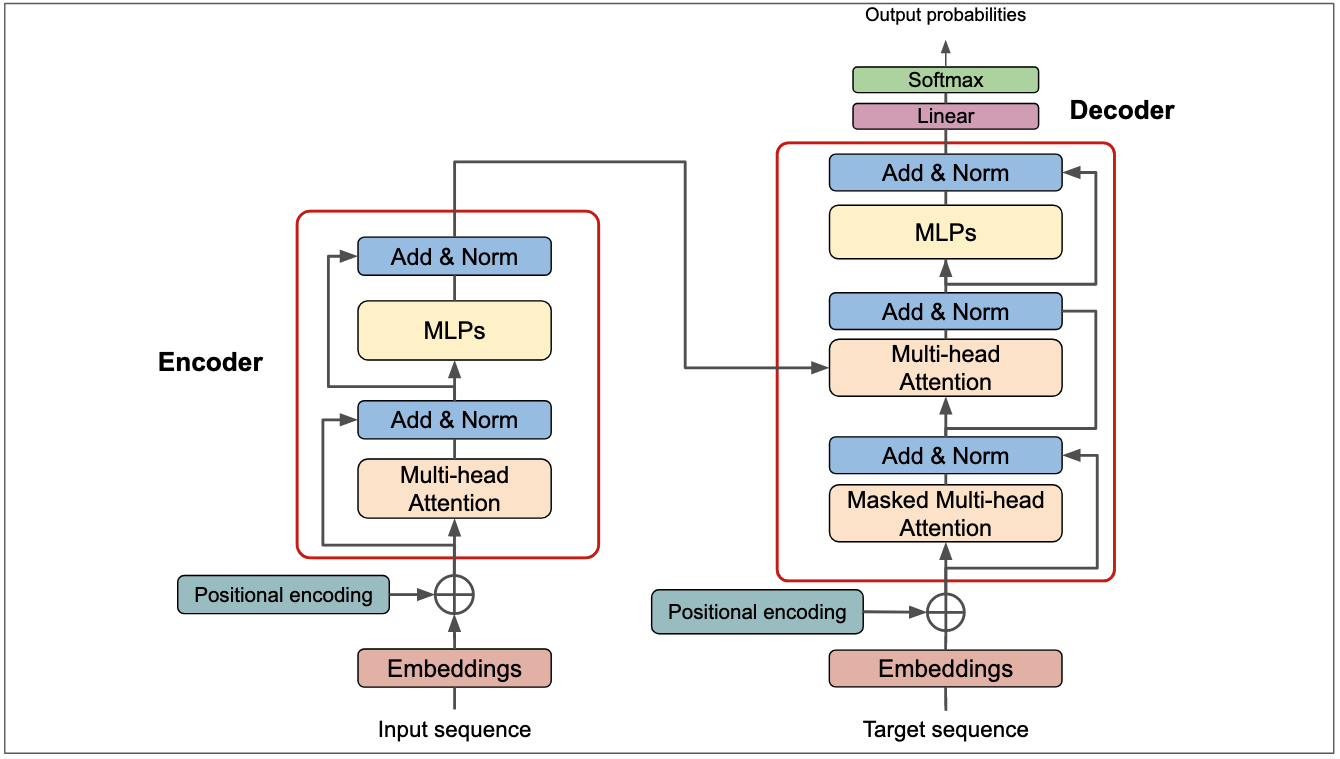
\includegraphics[width=140mm]{images/transformer}
	 	\caption{دیاگرام معماری ترنسفورمر }
	 	\label{fig_transformer}
	 \end{figure}
	 
	\item \textbf{مکانیزم توجه:}
	مکانیزم توجه به مدل‌ها اجازه می‌دهد تا به بخش‌های مختلف ورودی با وزن‌های متفاوت نگاه کنند و وابستگی‌های معنایی را بهتر درک نمایند. این مکانیزم به‌ویژه در ترجمه ماشینی و خلاصه‌سازی متون کاربرد دارد.
	
	\item \textbf{معماری‌های خودبازگشتی}
	\LTRfootnote{Autoregressive}
	\textbf{ و خودرمزگذار}
	 \LTRfootnote{Autoencoder}\textbf{:}
	\begin{itemize}
		\item 
	مدل‌های خودبازگشتی مانند سری GPT متن را به‌صورت ترتیبی تولید می‌کنند و هر کلمه را بر اساس کلمات قبلی پیش‌بینی می‌نمایند.
		\item 
	مدل‌های خودرمزگذار مانند BERT با استفاده از ماسک‌کردن کلمات در ورودی، سعی در درک زمینه و پیش‌بینی کلمات ماسک‌شده دارند.
	\end{itemize}
\end{enumerate}

\subsection{مدل بزرگ زبانی Mistral}


مدل بزرگ زبانی Mistral \cite{mistral} از جمله دستاوردهای جدید در حوزه پردازش زبان طبیعی به شمار می‌آید که با بهره‌گیری از معماری ترنسفورمر، عملکرد بالایی در وظایف متنوع زبانی نشان داده است. در ادامه به بررسی جامع این مدل می‌پردازیم.

مدل Mistral بر پایه معماری ترنسفورمر طراحی شده است. همانطور که گفته شد، این معماری با استفاده از مکانیزم توجه قادر است وابستگی‌های طولانی‌مدت در متون را به‌صورت موازی پردازش کند. از ویژگی‌های برجسته این مدل می‌توان به استفاده از تعداد پارامترهای بالا
\footnote{در این پژوهش از مدل‌های 7 میلیارد پارامتری استفاده شده است}
 اشاره کرد که موجب بهبود دقت و کیفیت تولید متن می‌شود.

برای رسیدن به عملکرد مطلوب، مدل Mistral با استفاده از مجموعه‌های داده گسترده و متنوع آموزش داده شده است. علاوه بر این، بهره‌گیری از تکنیک‌های تنظیم دقیق
\LTRfootnote{Fine-tuning}
 و بهینه‌سازی پیشرفته، موجب شده تا مدل بتواند در وظایف خاص، همچون ترجمه، خلاصه‌سازی و پاسخ به پرسش، عملکرد بهتری از خود نشان دهد.


مدل Mistral در حوزه‌های مختلف پردازش زبان طبیعی کاربرد دارد. از وظایف مهم آن می\/توان به توانایی تولید متونی با کیفیت بالا و طبیعی، ارائه ترجمه‌های دقیق و روان بین زبان‌ها، استخراج اطلاعات کلیدی و ارائه خلاصه‌های مفید از متون طولانی و همچنین درک دقیق سوالات و ارائه پاسخ‌های مرتبط و دقیق اشاره کرد.


با وجود این توانایی ها، مدل Mistral دارای نوآوری‌ها و مزایای متعددی نیز است که آن را از سایر مدل‌های زبانی متمایز می‌کند. این نوآوری ها شامل بهره‌گیری از معماری ترنسفورمر جهت پردازش موازی و بهبود سرعت محاسبات است، همچنین استفاده از تعداد پارامترهای بالا به افزایش دقت و کیفیت خروجی‌ها منجر می‌شود و قابلیت تنظیم دقیق برای تطبیق با وظایف خاص و کاربردهای صنعتی و پژوهشی را فراهم می آورد و به دنبال آن، بهبود چشمگیری در درک وابستگی‌های زبانی و تولید متون طبیعی حاصل می\/شود.


با وجود دستاوردهای قابل توجه، مدل Mistral همچنان با چالش‌هایی همچون مصرف بالای منابع محاسباتی و نیاز به داده‌های آموزشی گسترده مواجه است. پژوهش‌های آتی در زمینه بهبود کارایی، کاهش هزینه‌های محاسباتی و افزایش دقت در کاربردهای خاص، افق‌های روشن‌تری را برای این مدل ترسیم می‌کند.



\section{مهندسی اعلان}
مهندسی اعلان 
\LTRfootnote{Prompt Engineering}
 به فرآیند طراحی و بهینه‌سازی ورودی‌های متنی اطلاق می‌شود که به مدل‌های زبانی بزرگ ارائه می‌گردد تا خروجی‌های مطلوب و دقیقی تولید کنند. این ورودی‌ها می‌توانند شامل دستورات، سؤالات یا داده‌های زمینه‌ای باشند که به مدل کمک می‌کنند تا پاسخ‌های خود را در چارچوب معنایی و ساختاری مشخصی ارائه دهد.
می\/دانیم که مهندسی اعلان تأثیر مستقیمی بر کارایی و دقت مدل‌های زبانی بزرگ دارد از این رو با تدوین اعلان‌های دقیق و متناسب با وظیفه موردنظر، می‌توان رفتار مدل را به‌گونه‌ای هدایت کرد که خروجی‌های مرتبط‌تر و با کیفیت‌تری تولید کند. این امر به‌ویژه در شرایطی که داده‌های آموزشی محدود یا ناموجود هستند، اهمیت بیشتری پیدا می‌کند.
از مزایای مهندسی اعلان میتوان به موارد زیر اشاره کرد :
\begin{itemize}
	\item 
	با استفاده از اعلان‌های دقیق و مناسب می‌توان نتایج مدل را به سمت پاسخ‌های موردنظر هدایت کرد و کنترل بیشتری بر خروجی مدل داشت.
	\item 
	مهندسی اعلان می‌تواند به کاهش سوگیری‌های موجود در مدل‌های زبانی کمک کند و نتایج منصفانه‌تری ارائه دهد.
	\item 
	با تدوین اعلان‌های مؤثر، می‌توان زمان و منابع موردنیاز برای رسیدن به نتایج مطلوب را کاهش داد و کارایی را افزایش داد.
\end{itemize}

در نتیجه، مهندسی اعلان به‌عنوان ابزاری قدرتمند برای بهبود عملکرد مدل‌های زبانی بزرگ محسوب می‌شود و نقش کلیدی در توسعه و بهره‌برداری مؤثر از این مدل‌ها ایفا می‌کند.

\section{روش‌های دستی در مهندسی اعلان}
مهندسی اعلان دستی به فرآیند طراحی و بهینه‌سازی دستی ورودی‌ها (اعلان‌ها) برای هدایت بهتر مدل‌های زبانی بزرگ در تولید پاسخ‌های مطلوب گفته می‌شود. برخلاف روش‌های خودکار که از الگوریتم‌های یادگیری ماشین برای بهینه‌سازی اعلان‌ها استفاده می‌کنند، روش‌های دستی بر دانش زبانی، شهود انسانی و آزمایش‌های مکرر متکی هستند. این تکنیک‌ها در کاربردهای واقعی که نیاز به کنترل دقیق بر خروجی مدل دارند، مانند پاسخ‌گویی به سوالات، خلاصه‌سازی متون و انجام وظایف استدلالی، به‌کار گرفته می‌شوند.  

مهندسی اعلان دستی برای افزایش اثربخشی مدل‌های زبانی ضروری است، به‌ویژه در مواردی که تنظیم و آموزش مجدد مدل امکان‌پذیر نیست. از آنجایی که مدل‌های زبانی پاسخ‌های خود را بر اساس ورودی‌ها تولید می‌کنند، حتی تغییرات جزئی در ساختار یا نحوه بیان اعلان‌ها می‌تواند تأثیر قابل‌توجهی بر عملکرد آن‌ها داشته باشد. اعلان‌های طراحی‌شده به‌صورت بهینه می‌توانند دقت مدل را افزایش داده، توانایی استدلال آن را بهبود بخشند و میزان سوگیری در پاسخ‌ها را کاهش دهند، در نتیجه پاسخ‌های دقیق‌تر و متناسب‌تری ارائه کنند.

از ویژگی‌های کلیدی مهندسی اعلان دستی میتوان به موارد زیر اشاره کرد :
\begin{enumerate}
	\item طراحی مبتنی بر دانش انسانی 
	\begin{itemize}
		\item برخلاف روش‌های خودکار که از الگوریتم‌های بهینه‌سازی استفاده می‌کنند، مهندسی اعلان دستی بر شهود انسانی و دانش زبانی تکیه دارد.
		\item درک صحیح از زبان و زمینه موردنظر نقش مهمی در طراحی اعلان‌هایی دارد که مدل را به تولید خروجی‌های مطلوب هدایت می‌کنند. 
	\end{itemize}
	
	\item بهینه‌سازی تدریجی و تکرارشونده
	\begin{itemize}
		\item طراحی اعلان‌های مؤثر نیازمند آزمایش‌های مداوم و اصلاحات متوالی است. 
		\item تنظیمات و تغییرات مداوم در نحوه بیان اعلان به شناسایی بهترین ساختار و سبک ورودی کمک می‌کند. 
	\end{itemize}
	
	\item انعطاف‌پذیری در کاربردهای مختلف
	\begin{itemize}
		\item مهندسی اعلان دستی امکان شخصی‌سازی ورودی‌ها را برای وظایف متنوعی مانند تولید محتوا، برنامه‌نویسی و استدلال منطقی فراهم می‌کند.  
		\item استراتژی‌های خاصی را می‌توان برای هر کاربرد به‌کار گرفت، مانند ارائه دستورالعمل‌های گام‌به‌گام، اضافه کردن نشانه‌های متنی یا استفاده از نمونه‌های مشابه.
	\end{itemize}
	
	\item کنترل و تفسیرپذیری بهتر
	\begin{itemize}
		\item از آنجا که اعلان‌های دستی توسط انسان طراحی می‌شوند، کنترل بیشتری بر رفتار مدل فراهم می‌کنند.  
		\item این روش امکان درک بهتر نحوه پاسخ‌گویی مدل به ورودی‌های مختلف را فراهم کرده و به عیب‌یابی و بهبود عملکرد کمک می‌کند.
	\end{itemize}
\end{enumerate}

با وجود مزایای فراوان، این روش با چالش‌هایی همراه است:  
\begin{itemize}
	\item فرآیند زمان‌بر: طراحی و بهینه‌سازی دستی اعلان‌ها نیاز به صرف زمان زیادی دارد.  
	\item مقیاس‌پذیری پایین: برخلاف روش‌های خودکار، اعلان‌های دستی به‌راحتی برای مدل‌ها یا وظایف دیگر تعمیم نمی‌یابند.  
	\item ماهیت مبتنی بر آزمون و خطا: یافتن اعلان بهینه اغلب نیازمند آزمایش‌های متعدد است که همیشه نتیجه‌ای ثابت و پایدار را تضمین نمی‌کند.  
\end{itemize}

در نهایت مهندسی اعلان دستی به‌عنوان رویکردی بنیادین برای بهینه‌سازی تعاملات با مدل‌های زبانی شناخته می‌شود. در بخش‌های بعدی، روش‌های مختلف مهندسی اعلان دستی را بررسی خواهیم کرد و تأثیر هر یک را بر توانایی‌های استدلالی و کیفیت پاسخ‌دهی مدل می‌سنجیم.
%بررسی کاربرد و مزایا و معایب این روش‌ها
\subsection{یادگیری درون متنی}

یادگیری درون‌متنی
\LTRfootnote{In-Context Learning}
 از قابلیت‌های برجسته مدل‌های زبانی بزرگ است که به آن‌ها اجازه می‌دهد بدون نیاز به بازآموزی
 \LTRfootnote{Training}
  یا تنظیم مجدد وزن‌ها، تنها با دریافت چند نمونه در ورودی، وظایف جدید را تشخیص دهند و به درستی انجام دهند. این روش به مدل کمک می‌کند با تحلیل مثال‌های ارائه‌شده در ورودی، پاسخ‌هایی متناسب با همان زمینه تولید کند.
از مزایای مهم این روش، افزایش انعطاف‌پذیری در مواجهه با وظایف و موضوعات جدید است که باعث می\/شود مدل‌های زبانی به سرعت خود را با زمینه‌های مختلف تطبیق دهند. با حذف نیاز به بازآموزی برای هر وظیفه جدید، این روش می‌تواند بهینه‌سازی قابل توجهی در مصرف منابع و زمان ایجاد کند.
از سوی دیگر، این قابلیت نقش مهمی در بهبود کیفیت تعاملات میان انسان و ماشین ایفا می‌کند. مدل‌ها با درک بهتر زمینه و مثال‌های ارائه‌شده، پاسخ‌هایی طبیعی‌تر و دقیق‌تر تولید می‌کنند که باعث افزایش رضایت کاربران می‌شود.

با وجود مزایای فوق، یادگیری درون‌متنی با چالش‌هایی نیز همراه است. عملکرد مدل‌ها به شدت به کیفیت و تنوع داده‌ها و مثال‌های ورودی وابسته است. مثال‌های ناقص یا ناسازگار می‌توانند منجر به تولید پاسخ‌های نادرست شوند. همچنین، در برخی موقعیت‌های پیچیده یا مبهم، مدل ممکن است در درک دقیق زمینه دچار مشکل شود. 


از روش های یادگیری درون متنی میتوان به یادگیری بدون نمونه و یادگیری با نمونه های کم اشاره کرد. در یادگیری بدون نمونه 
\cite{ZSL}
\LTRfootnote{Zero-Shot Learning (ZSL)}
  مدل‌ها وظیفه دارند اشیاء یا مفاهیمی را که در طول آموزش با آن‌ها روبرو نشده‌اند شناسایی و دسته‌بندی کنند. برخلاف یادگیری نظارت‌شده سنتی که نیاز به مثال‌های برچسب‌خورده برای هر کلاس دارد، یادگیری بدون نمونه به مدل‌ها این امکان را می‌دهد که پیش‌بینی‌هایی در مورد دسته‌های دیده نشده در زمان آموزش با استفاده از اطلاعات کمکی انجام دهند.  
برای شناسایی کلاس‌های دیده نشده در زمان آموزش، مدل‌های یادگیری بدون نمونه روابطی بین کلاس‌های مشاهده‌شده (دیده‌شده) و کلاس‌های مشاهده‌نشده (دیده‌ نشده) برقرار می‌کنند. این ارتباط معمولاً از طریق ویژگی‌های مشترک یا اطلاعات معنایی که این دو را به هم پیوند می‌دهند، تسهیل می‌شود.  
از طرفی وجود اطلاعات کمکی برای یادگیری بدون نمونه حیاتی است و  داده‌های توصیفی در مورد کلاس‌های دیده‌شده و دیده نشده ارائه می‌دهد. این اطلاعات می‌تواند شامل ویژگی‌هایی مانند توضیحات متنی، جاسازی‌های معنایی یا سایر داده‌های مرتبط باشد که به مدل کمک می‌کند تا کلاس‌ها را درک کرده و از هم تمایز دهد. 

چگونگی عملکرد یادگیری بدون نمونه بدین صورت است که در غیاب مثال‌های برچسب‌خورده برای کلاس‌های دیده نشده، برای پر کردن شکاف به اطلاعات کمکی اتکا می\/کنند. به عنوان مثال، در طبقه‌بندی تصاویر، مدلی که بر اساس گونه‌های خاص حیوانات آموزش دیده باشد، می‌تواند از توضیحات متنی گونه‌های دیده نشده برای شناسایی صحیح آن‌ها استفاده کند. با درک اینکه یک گورخر مشابه یک اسب است اما با خطوط راه‌راه، مدل می‌تواند گورخرها را بدون دیدن آن‌ها در طول آموزش شناسایی کند (تصویر \ref{fig_zil}).

\begin{figure}[!t]
	\centering
	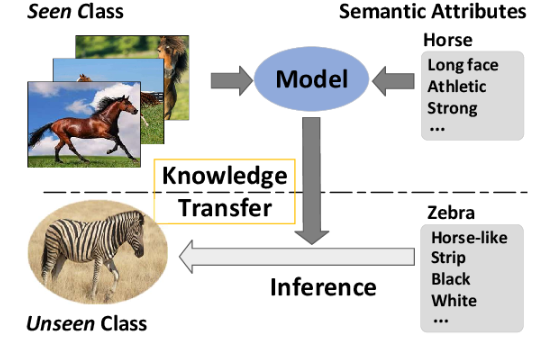
\includegraphics[width=100mm]{images/ZeroShot}
	\caption{مثالی از یادگیری بدون نمونه در یادگیری درون متنی}
	\label{fig_zil}
\end{figure}

یادگیری بدون نمونه در حوزه‌های مختلفی کاربرد داشته است، از جمله:
\begin{itemize}
	\item 
	طبقه‌بندی تصویر: شناسایی اشیاء یا گونه‌هایی که در داده‌های آموزشی وجود ندارند.
	\item 
	بخش‌بندی معنایی: بخش‌بندی اشیاء دیده نشده در تصاویر بر اساس ویژگی‌های یادگرفته‌شده.
	\item 
	پردازش زبان طبیعی: انجام کارهایی مانند طبقه‌بندی متن یا شناسایی موجودیت‌ها بدون مثال‌های صریح.
	\item 
	زیست‌شناسی محاسباتی: پیش‌بینی عملکرد ژن‌ها یا پروتئین‌هایی که فاقد نشانه‌های آزمایشی هستند.  
\end{itemize}

از چالش‌های مهم یادگیری بدون نمونه می\/توان به احتمال اشتباه کردن مدل در دسته‌بندی کلاس‌های دیده نشده اشاره کرد، به ویژه زمانی که این کلاس‌ها ویژگی‌هایی مشابه با کلاس‌های دیده‌شده دارند. تحقیقات جاری به دنبال افزایش کارایی و دقت مدل‌های یادگیری بدون نمونه است و روش‌هایی مانند تولید داده‌های مصنوعی برای کلاس‌های دیده نشده و بهبود کیفیت اطلاعات کمکی را بررسی می‌کنند.

در طرف دیگر ماجرا، برای یادگیری با نمونه های کم \cite{FSL} مدل‌ها طوری طراحی می‌شوند که بتوانند بر اساس تعداد بسیار محدودی از نمونه‌های آموزشی، یادگیری کرده و پیش‌بینی‌های دقیقی انجام دهند. این رویکرد به‌ویژه در موقعیت‌هایی مفید است که جمع‌آوری مجموعه‌داده‌های بزرگ عملی یا مقرون‌به‌صرفه نیست.

در یادگیری با نمونه های کم، مدل‌ها در مرحله استنتاج تنها تعداد کمی نمونه برچسب‌خورده (که اغلب به آن مجموعه پشتیبان
\LTRfootnote{support set}
 گفته می‌شود) برای هر کلاس جدید دریافت می‌کنند. این تعداد محدود از نمونه‌ها به مدل امکان می‌دهد تا به سرعت خود را تطبیق داده و برای کلاس‌های نادیده‌شده پیش‌بینی انجام دهد.

یک تنظیم رایج در یادگیری با نمونه های کم شامل الگوی N-way K-shot است که در آن 'N' نشان‌دهنده تعداد کلاس‌های جدید و 'K' نشان‌دهنده تعداد نمونه‌های برچسب‌خورده موجود برای هر کلاس است. برای مثال، در یک سناریوی 5-way 1-shot، پنج کلاس جدید وجود دارد که هر کدام تنها یک نمونه برچسب‌خورده دارند.

مدل‌های یادگیری با نمونه های کم معمولاً از تکنیک‌های فرا-یادگیری 
\LTRfootnote{meta Learning}
 استفاده می‌کنند که به آن "یادگیری برای یادگیری
 \LTRfootnote{Learning to Learn}
 " نیز گفته می‌شود. در این چارچوب، مدل در طیف وسیعی از وظایف آموزش می‌بیند تا یک استراتژی برای تطبیق سریع با وظایف جدید با حداقل داده‌ها را یاد بگیرد. در زمان استنتاج، مدل با استفاده از همان تعداد اندک نمونه‌ها، پارامترهای خود را به‌طور مؤثری تنظیم می‌کند و می‌تواند دسته‌بندی‌های جدید را شناسایی و طبقه‌بندی کند.

از کاربردهای یادگیری با نمونه‌های کم می\/توان به موارد زیر اشاره کرد:
\begin{itemize}
	\item 
	یادگیری با نمونه‌های کم به مدل‌ها امکان می‌دهد تصاویر را با استفاده از تنها چند نمونه برچسب‌خورده در دسته‌های جدید طبقه‌بندی کنند که این موضوع به‌ویژه در حوزه‌هایی مانند تصویربرداری پزشکی که برچسب‌گذاری داده‌ها بسیار زمان‌بر است، اهمیت دارد.
	\item 
	در حوزه پردازش زبان طبیعی، یادگیری با نمونه‌های کم می‌تواند در وظایفی مانند طبقه‌بندی متن و تحلیل احساسات به کار رود و به مدل‌ها کمک کند تا با حداقل داده متنی، موضوعات جدید را پردازش و درک کنند.
	\item 
	ربات‌ها می‌توانند با استفاده از یادگیری با نمونه‌های کم وظایف جدید در زمینه دست‌کاری اشیاء یا تطبیق با محیط‌های تازه را یاد بگیرند، که این موضوع نیاز به آموزش مجدد گسترده را کاهش داده و امکان استقرار سریع در محیط‌های پویا را فراهم می‌آورد.
\end{itemize}

یکی از چالش‌های اصلی در یادگیری با نمونه‌های کم این است که اطمینان حاصل شود مدل‌ها خود را با داده‌های محدودبه‌خوبی تعمیم می‌دهند و دچار بیش‌برازش
\LTRfootnote{overfitting}
 نمی‌شوند. پژوهشگران در حال بررسی روش‌های مختلفی از جمله افزایش داده 
 \LTRfootnote{data augmentation}
 ، یادگیری انتقالی
 \LTRfootnote{transfer learning}
  و الگوریتم‌های پیشرفته فرا-یادگیری
  \LTRfootnote{meta Learning}
   برای بهبود عملکرد مدل‌های یادگیری با نمونه‌های کم هستند.

برای فهم شفاف تر روش یادگیری درون متنی میتوان از یک چهارچوب ریاضیاتی
\cite{beysian}
 کمک گرفت. در این چارچوب ریاضیاتی می\/توان یادگیری درون‌متنی را به‌عنوان یک استنتاج بیزی ضمنی
\LTRfootnote{implicit Bayesian inference}
 تفسیر کرد. در چارچوب آن‌ها، در طی پیش‌آموزش
 \LTRfootnote{pre-training}
 ، مدل‌های زبانی بزرگ با استنتاج مفاهیم پنهان در اعلان، که روابط معنایی و نحوی مختلفی را در متن در بر می‌گیرد، یاد می‌گیرند که توکن‌های بعدی را پیش‌بینی کنند. در زمان استنتاج
 \LTRfootnote{inference time}
 ، زمانی که مدلی با یک اعلان شامل مثال‌های ورودی-خروجی مواجه می‌شود، یک مفهوم پنهان مشترک بین این مثال‌ها را شناسایی می‌کند. این فرآیند شناسایی با استنتاج بیزی هم‌راستا است، جایی که مدل بر اساس داده‌های مشاهده‌شده، باورهای خود را به‌روزرسانی می‌کند تا پیش‌بینی انجام دهد.

\begin{equation}\label{eq_icl}
	P(\text{خروجی} \mid \text{اعلان}) = \int P(\text{خروجی} \mid \text{مفهوم}) \cdot P(\text{اعلان} \mid \text{مفهوم}) \cdot P( \text{مفهوم}) \, d \text{مفهوم}
\end{equation}



همانطور که در معادله \ref{eq_icl} مشاهده می\/شود، از منظر بیزی، یادگیری درون متنی با پیدا کردن احتمال خروجی به شرط اعلان برابر است که انجام استنتاج توسط مدل برای یافتن یک مفهوم پنهان را در بر می\/گیرد که این مفهوم با وظیفه مورد نظر همخوانی دارد. با دریافت یک اعلان، مدل توزیع پسین
\LTRfootnote{posterior}
 را بر روی مفاهیم پنهان ممکن استنتاج می‌کند و مفهومی را انتخاب می‌کند که به بهترین نحو مثال‌های ارائه‌شده را توضیح می‌دهد. این فرآیند مشابه به‌روزرسانی بیزی است که در آن باورهای قبلی در پرتو شواهد جدید تنظیم می‌شوند تا پیش‌بینی‌های آگاهانه‌تری انجام گیرد.

\subsection{روش زنجیره تفکر}
روش زنجیره تفکر
\LTRfootnote{Chain-of-Thought} \cite{CoT}
 تکنیکی است که با هدف تقویت توانایی استدلال مدل‌های زبانی بزرگ طراحی شده و آن‌ها را راهنمایی می‌کند تا هنگام حل مسائل پیچیده، گام‌های میانی استدلالی تولید کنند. این رویکرد مدل‌ها را تشویق می‌کند تا وظایف را به بخش‌های متوالی و مرحله‌به‌مرحله تقسیم کرده و در نتیجه به خروجی‌هایی دقیق‌تر و قابل تفسیرتر برسند.

این روش که توسط پژوهشگران گوگل معرفی شد، شامل ارائه نمونه‌هایی به مدل‌ها است که هم شامل مسئله و هم شامل راه‌حل گام‌به‌گام و دقیق هستند. به عنوان مثال، وقتی یک مسئله کلامی ریاضی به مدل داده می‌شود، مدل با استفاده از زنجیره تفکر تشویق می‌شود که محاسبات و مراحل منطقی منتهی به پاسخ نهایی را به صورت شفاف بیان کند. این روش نشان داده که عملکرد مدل‌ها را در وظایف نیازمند به محاسبات ریاضی، استدلال مبتنی بر عقل سلیم و استدلال نمادین به شکل چشمگیری بهبود می‌دهد. به طور خاص، یک مدل با ۵۴۰ میلیارد پارامتر با استفاده از CoT موفق شد به دقتی فراتر از حد استاندارد در دیتاست GSM8K برای مسائل ریاضی دست پیدا کند و حتی بهتر از نسخه‌های تنظیم شده GPT-3 عمل کند.

اثربخشی روش زنجیره تفکر به‌ویژه در مدل‌های بزرگ‌تر بیشتر مشهود است. مدل‌هایی با بیش از ۱۰۰ میلیارد پارامتر در مواجهه با زنجیره تفکر توانایی‌های نوظهوری در زمینه استدلال چند مرحله‌ای از خود نشان می‌دهند و می‌توانند مسائل چند گامی را به شکل موثرتری حل کنند. این تکنیک نه تنها دقت را افزایش می‌دهد، بلکه شفافیت فرآیند استدلال مدل را نیز بهبود می‌بخشد؛ چرا که هر گام به صورت صریح ارائه می‌شود.

در شکل \ref{fig_cot} یک نمونه از تولید جواب با استفاده از روش زنجیره تفکر آورده شده است. در این مثال به عنوان ورودی یک سوال و جواب نمونه به همراه راه حل قدم به قدم مسئله نیز آورده شده است تا مدل به سمت تولید راه حل سوق داده شود.
\begin{figure}[!t]
	\centering
	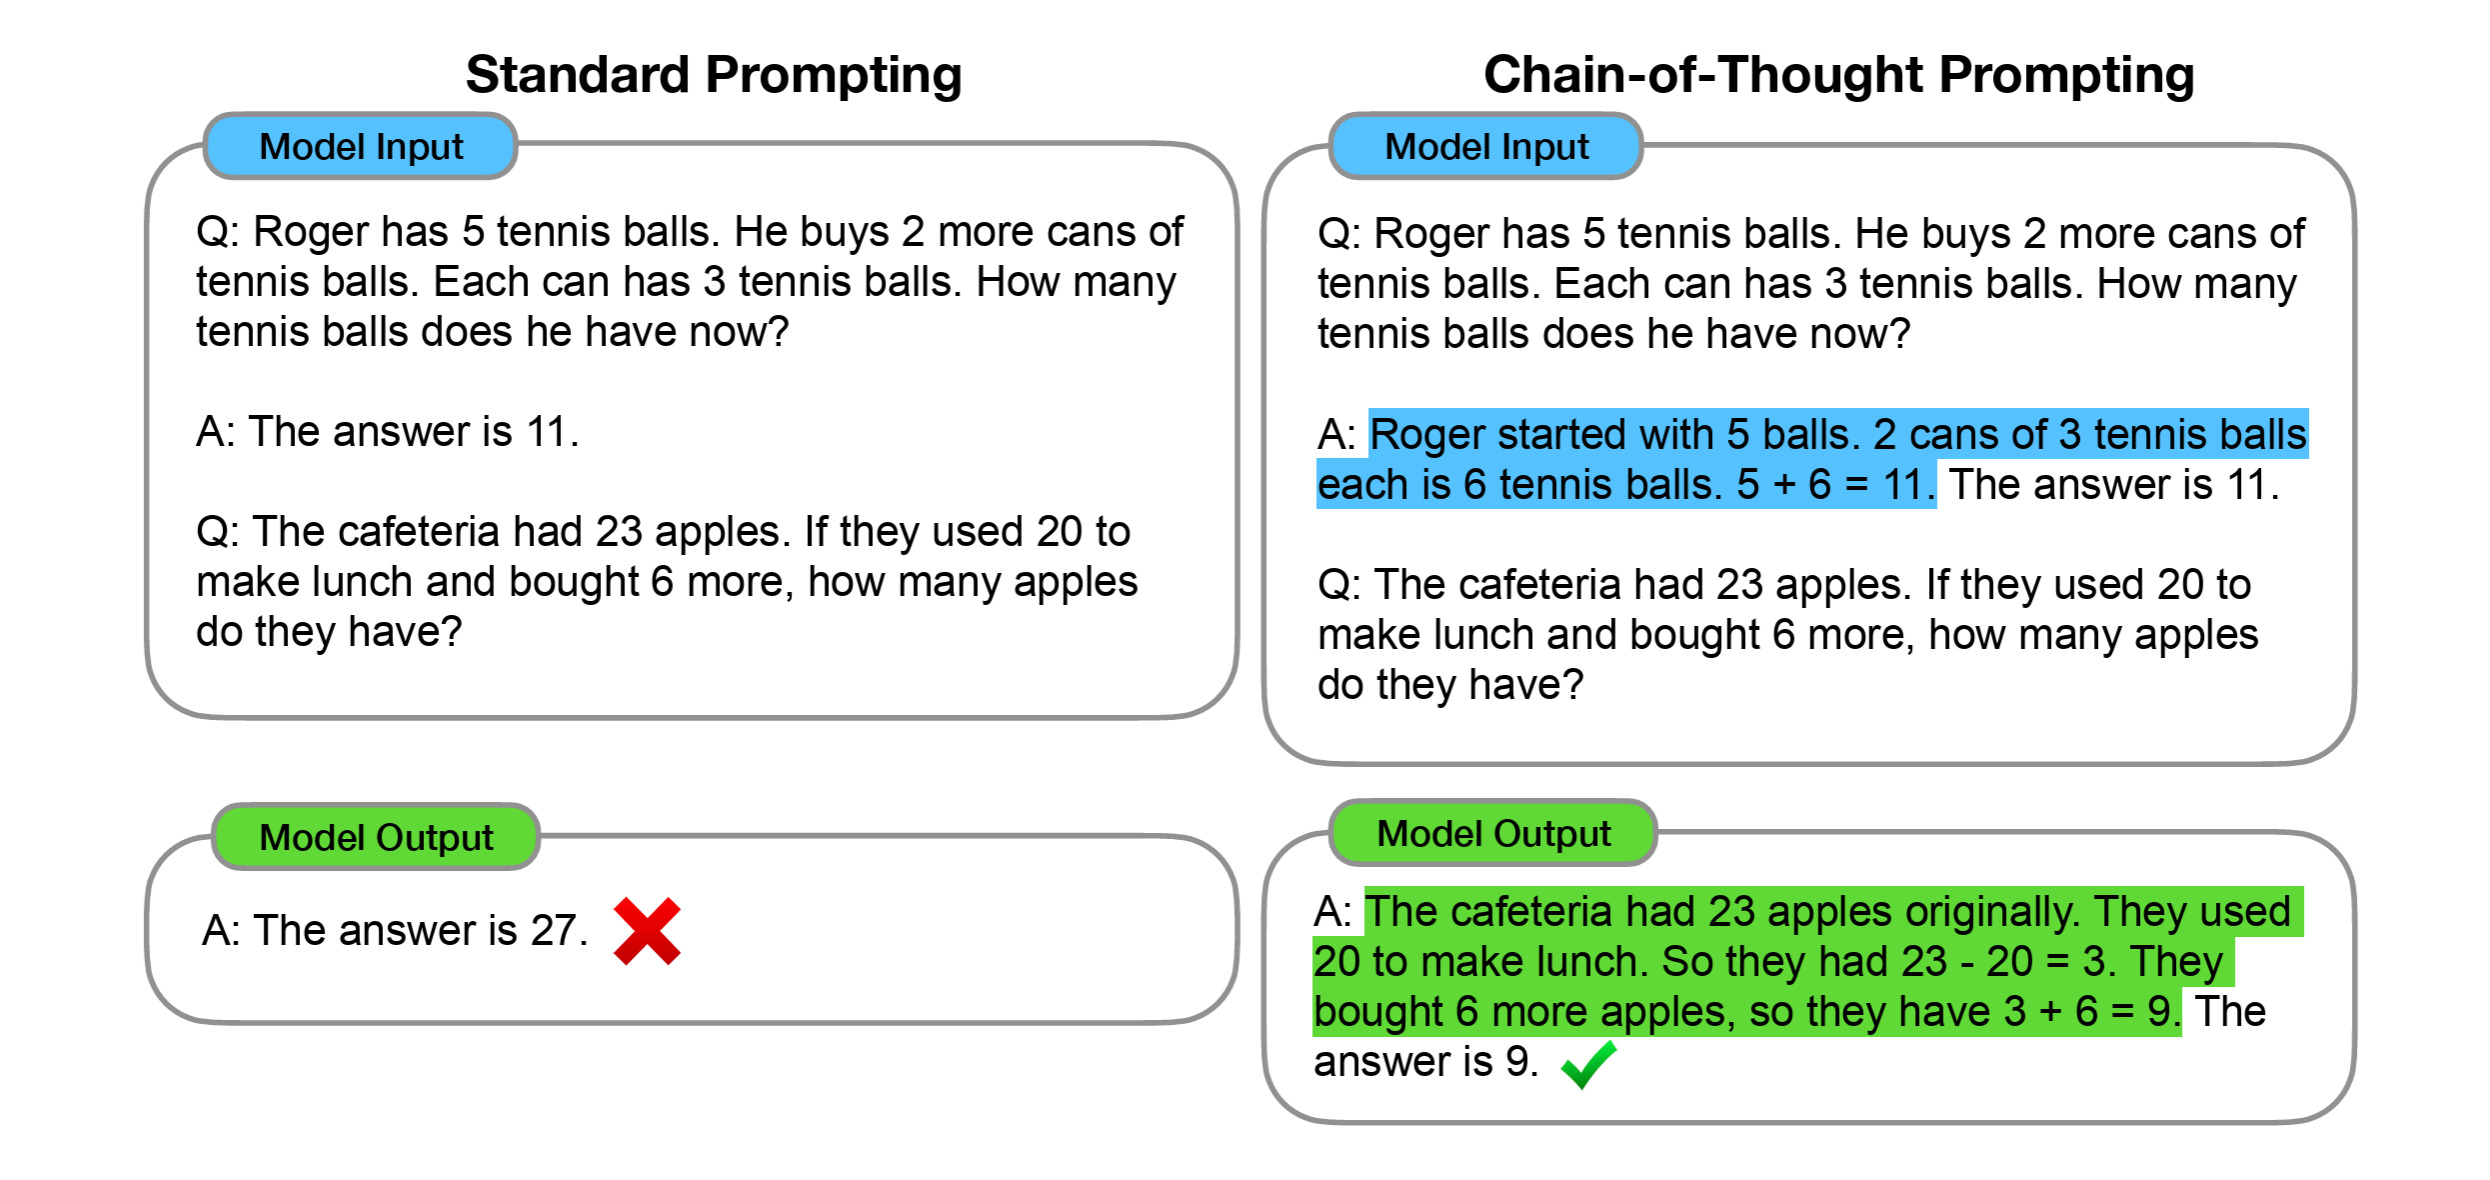
\includegraphics[width=140mm]{images/Cot}
	\caption{مثالی از روش زنجیره تفکر برای حل یک سوال از دیتاست \lr{GSM8K}}
	\label{fig_cot}
\end{figure}

\subsection{روش استدلال بدون دیدن نمونه آموزشی} 
در مقاله‌ی استدلال بدون دیدن نمونه آموزشی
\LTRfootnote{Large Language Models are Zero-Shot Reasoners} \cite{LLMzeroshot}
، پتانسیل مدل های بزرگ زبانی را برای انجام استدلال  از طریق تغییرات ساده در اعلان‌ها و بدون افزودن نمونه ای از مثال های حل شده، بررسی شده است. با اضافه کردن عبارت «بیایید مرحله به مرحله فکر کنیم» به انتهای یک اعلان، مدل‌هایی مانند GPT-3 و PaLM
\cite{palm2}
به‌طور قابل توجهی عملکرد بهتری در دیتاست‌های مختلف استدلالی ارائه می‌دهند. 
این روش بر توانایی ذاتی مدل‌ها در پردازش و تولید متن شبیه به انسان تکیه دارد و آن‌ها را تشویق می‌کند تا دنباله‌ای منطقی از تفکرات را که منجر به پاسخ نهایی می‌شود، تولید کنند. سادگی و کارآمدی این تکنیک، توانایی‌های استدلالی نهفته در مدل های بزرگ زبانی را آشکار می‌کند که می‌توان آن‌ها را بدون نیاز به آموزش وسیع و خاص برای هر وظیفه فعال کرد.
این یافته نشان می‌دهد که با مهندسی اعلان مناسب، این مدل‌ها می‌توانند طیف وسیعی از وظایف را به‌طور مؤثرتری انجام دهند و نیاز به دیتاست‌های بزرگ و برچسب‌گذاری شده و همچنین فرایندهای زمان‌بر تنظیم دقیق مدل‌ها را کاهش دهند. در شکل \ref{fig_zerocot} نمونه از حل مسئله دیتاست \lr{GSM8K} آورده شده است و جواب این روش با روش زنجیره تفکر مقایسه شده است.

\begin{figure}[!t]
	\centering
	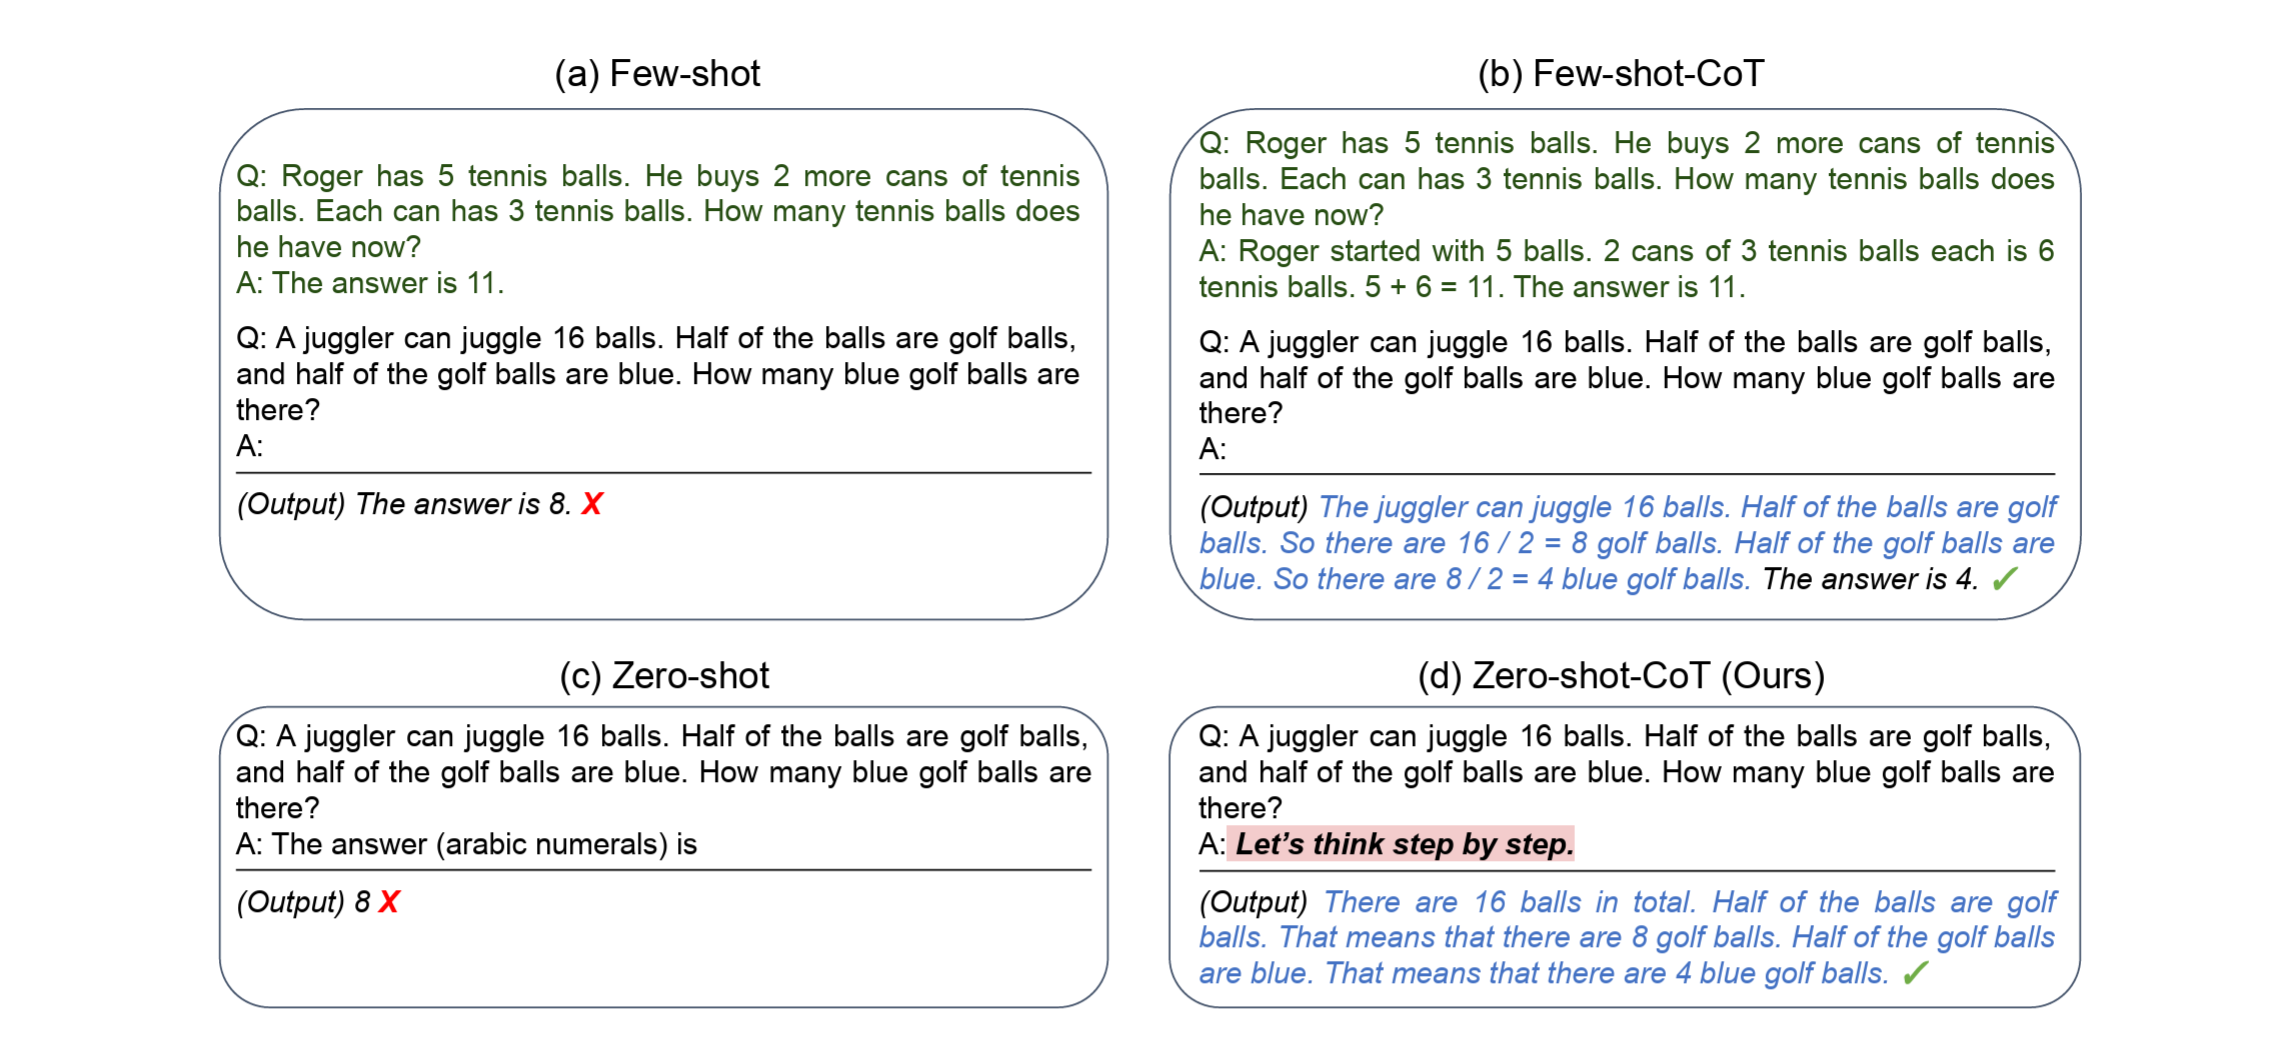
\includegraphics[width=140mm]{images/zerocot}
	\caption{مقایسه روش استدلال بدون دیدن نمونه آموزشی و روش زنجیره تفکر}
	\label{fig_zerocot}
\end{figure}


\subsection{روش برنامه تفکر}
روش برنامه تفکر
\LTRfootnote{Program-of-Thought} \cite{PoT}
یک روش پیشرفته در مهندسی اعلان است که برای بهبود توانایی‌های استدلال عددی در مدل‌های زبانی بزرگ طراحی شده است. برخلاف تکنیک زنجیره تفکر که در آن مدل هم استدلال و هم محاسبات را در قالب متن تولید می‌کرد، در برنامه تفکر این دو فرآیند از یکدیگر جدا می‌شوند. در این روش، مدل استدلال خود را به صورت کد قابل اجرایی (معمولاً با زبان‌هایی مانند پایتون) بیان می‌کند و این کد توسط یک مفسر خارجی اجرا می‌شود تا پاسخ نهایی به دست آید. این جداسازی باعث می‌شود محاسبه و استدلال از یکدیگر تفکیک شوند.

از مزایای روش برنامه تفکر می\/توان به موارد زیر اشاره کرد:
\begin{itemize}
	\item 
	با واگذاری محاسبات به یک مفسر خارجی، احتمال بروز خطاهای عددی که ممکن است در صورت انجام محاسبه و استدلال توسط خود مدل رخ دهد، کاهش می‌یابد و دقت بالاتر می\/رود.
	\item 
	مطالعات تجربی نشان داده‌اند که برنامه تفکر می‌تواند عملکرد مدل را در وظایف عددی پیچیده به طور قابل توجهی افزایش دهد. برای مثال، آزمایش‌ها نشان داده‌اند که PoT نتایجی هم‌سطح با بهترین روش‌های موجود در دیتاست‌های مسائل ریاضی و نزدیک به بهترین عملکردها در دیتاست‌های مالی داشته است.
	\item 
	نمایش مراحل استدلال به صورت کد، شفافیت فرآیند حل مسئله را افزایش می‌دهد و بررسی و درک هر مرحله را ساده‌تر می‌کند.
\end{itemize}

در شکل \ref{fig_pot} حل مسئله دنباله فیبونانچی و پیداکردن 50\/امین عضو این دنباله، با استفاده از روش زنجیره تفکر و روش برنامه تفکر بررسی شده است. به دلیل طولانی بودن مراحل حل مسئله، روش زنجیره تفکر نتوانسته جواب درست را پیدا کند ولی روش برنامه تفکر ابتدا یک کد برای حل این مسئله ارائه داده است و پس از اجرای این کد با مفسر، به جواب صحیح رسیده است.

\begin{figure}[!t]
	\centering
	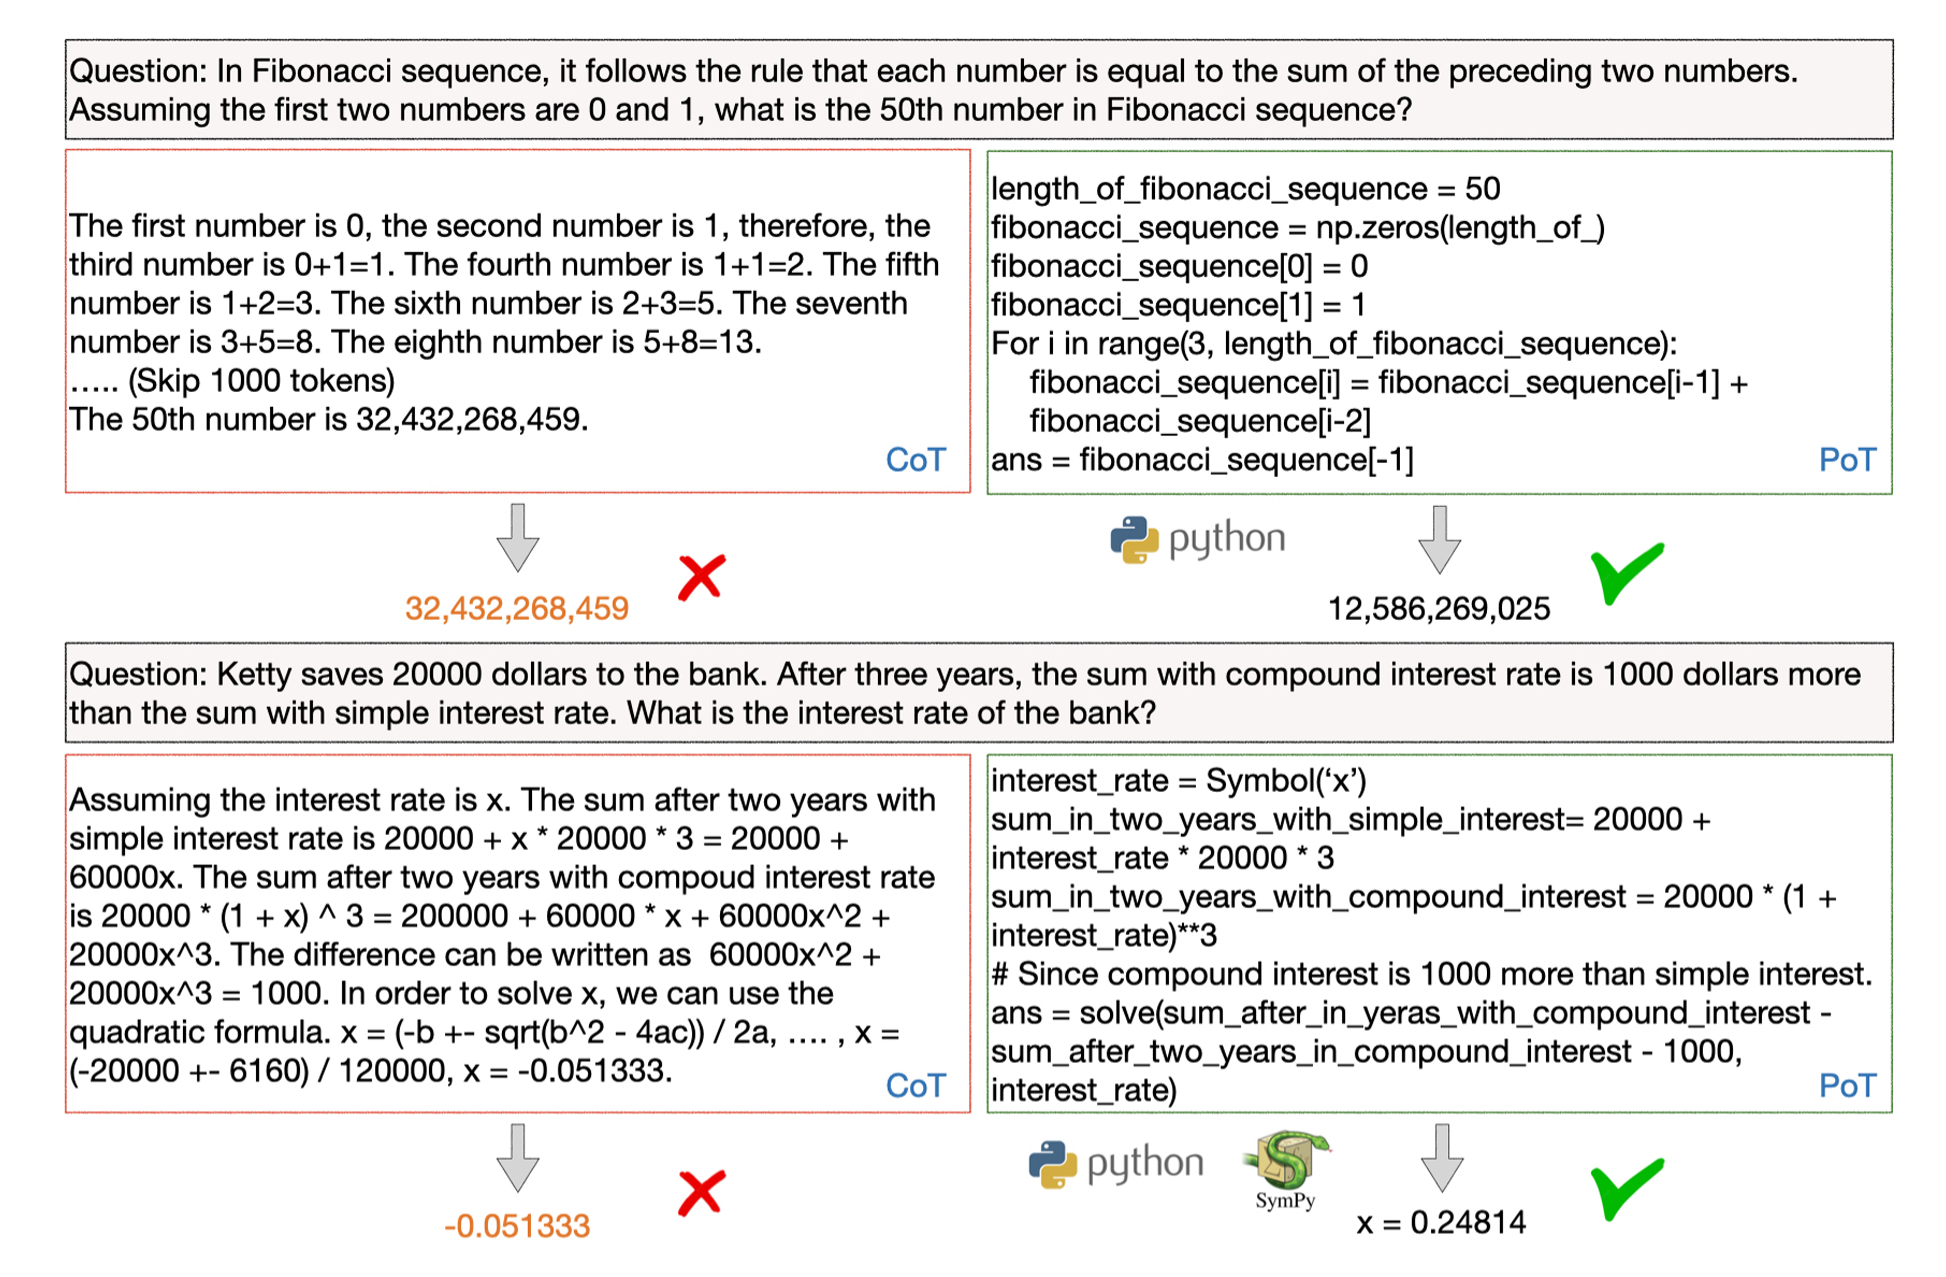
\includegraphics[width=140mm]{images/pot}
	\caption{مقایسه روش برنامه تفکر و روش زنجیره تفکر}
	\label{fig_pot}
\end{figure}

\subsection{روش بهینه سازی با اعلان}
همانطور که گفته شد مدل‌های زبانی بزرگ تا به اینجا برای وظایفی مانند تولید متن، ترجمه و خلاصه‌سازی به کار گرفته می‌شدند. با این حال، تحقیقات اخیر ظرفیت این مدل‌ها را به‌عنوان بهینه‌سازها مورد بررسی قرار داده‌اند و از قابلیت‌های استدلالی آن‌ها برای حل مسائل پیچیده بهینه‌سازی بهره برده‌اند.

یکی از رویکردهای برجسته در این زمینه، روش بهینه سازی با اعلان 
\LTRfootnote{Optimization by PROmpting} \cite{opro}
 است. این روش از مدل‌های زبانی بزرگ برای تولید راه‌حل‌های مسائل بهینه‌سازی بر اساس اعلان‌های زبان طبیعی استفاده می‌کند. این فرآیند شامل تکرارهای پی‌در‌پی است که در آن، اعلان جدید با راه‌حل‌ها و ارزیابی‌های قبلی طراحی می‌شود و در تکرارهای بعدی، راه‌حل‌های بهتری پیشنهاد می‌دهد. این روش در کاربردهای مختلفی همچون رگرسیون خطی
 \LTRfootnote{Linear Regression}
 ، مسئله فروشنده دوره‌گرد
 \LTRfootnote{Traveling Salesman Problem}
  و حتی بهینه‌سازی اعلان برای خود مدل‌های زبانی بزرگ مؤثر واقع شده است. جالب توجه اینکه این روش توانسته تا ۸٪ بهبود عملکرد در دیتاست \lr{GSM8K} و تا ۵۰٪ بهبود در وظایف دشوار
  \LTRfootnote{Big-Bench Hard}
   داشته باشد و حتی از اعلان‌های طراحی‌شده توسط انسان نیز پیشی بگیرد.

در روش بهینه سازی با اعلان، مسئله بهینه‌سازی با زبان طبیعی توصیف می‌شود تا مدل بتواند بافت و هدف مسئله را درک کند. همانطور که در شکل \ref{fig_opro} در هر مرحله از بهینه‌سازی، مدل با توجه به اعلان شامل راه‌حل‌ها و ارزیابی‌های قبلی، راه‌حل‌های جدیدی تولید می‌کند. این راه‌حل‌ها ارزیابی شده و سپس برای تکرار بعدی در اعلان گنجانده می‌شوند و این چرخه بهبود مستمر ادامه پیدا می‌کند.

\begin{figure}[!t]
	\centering
	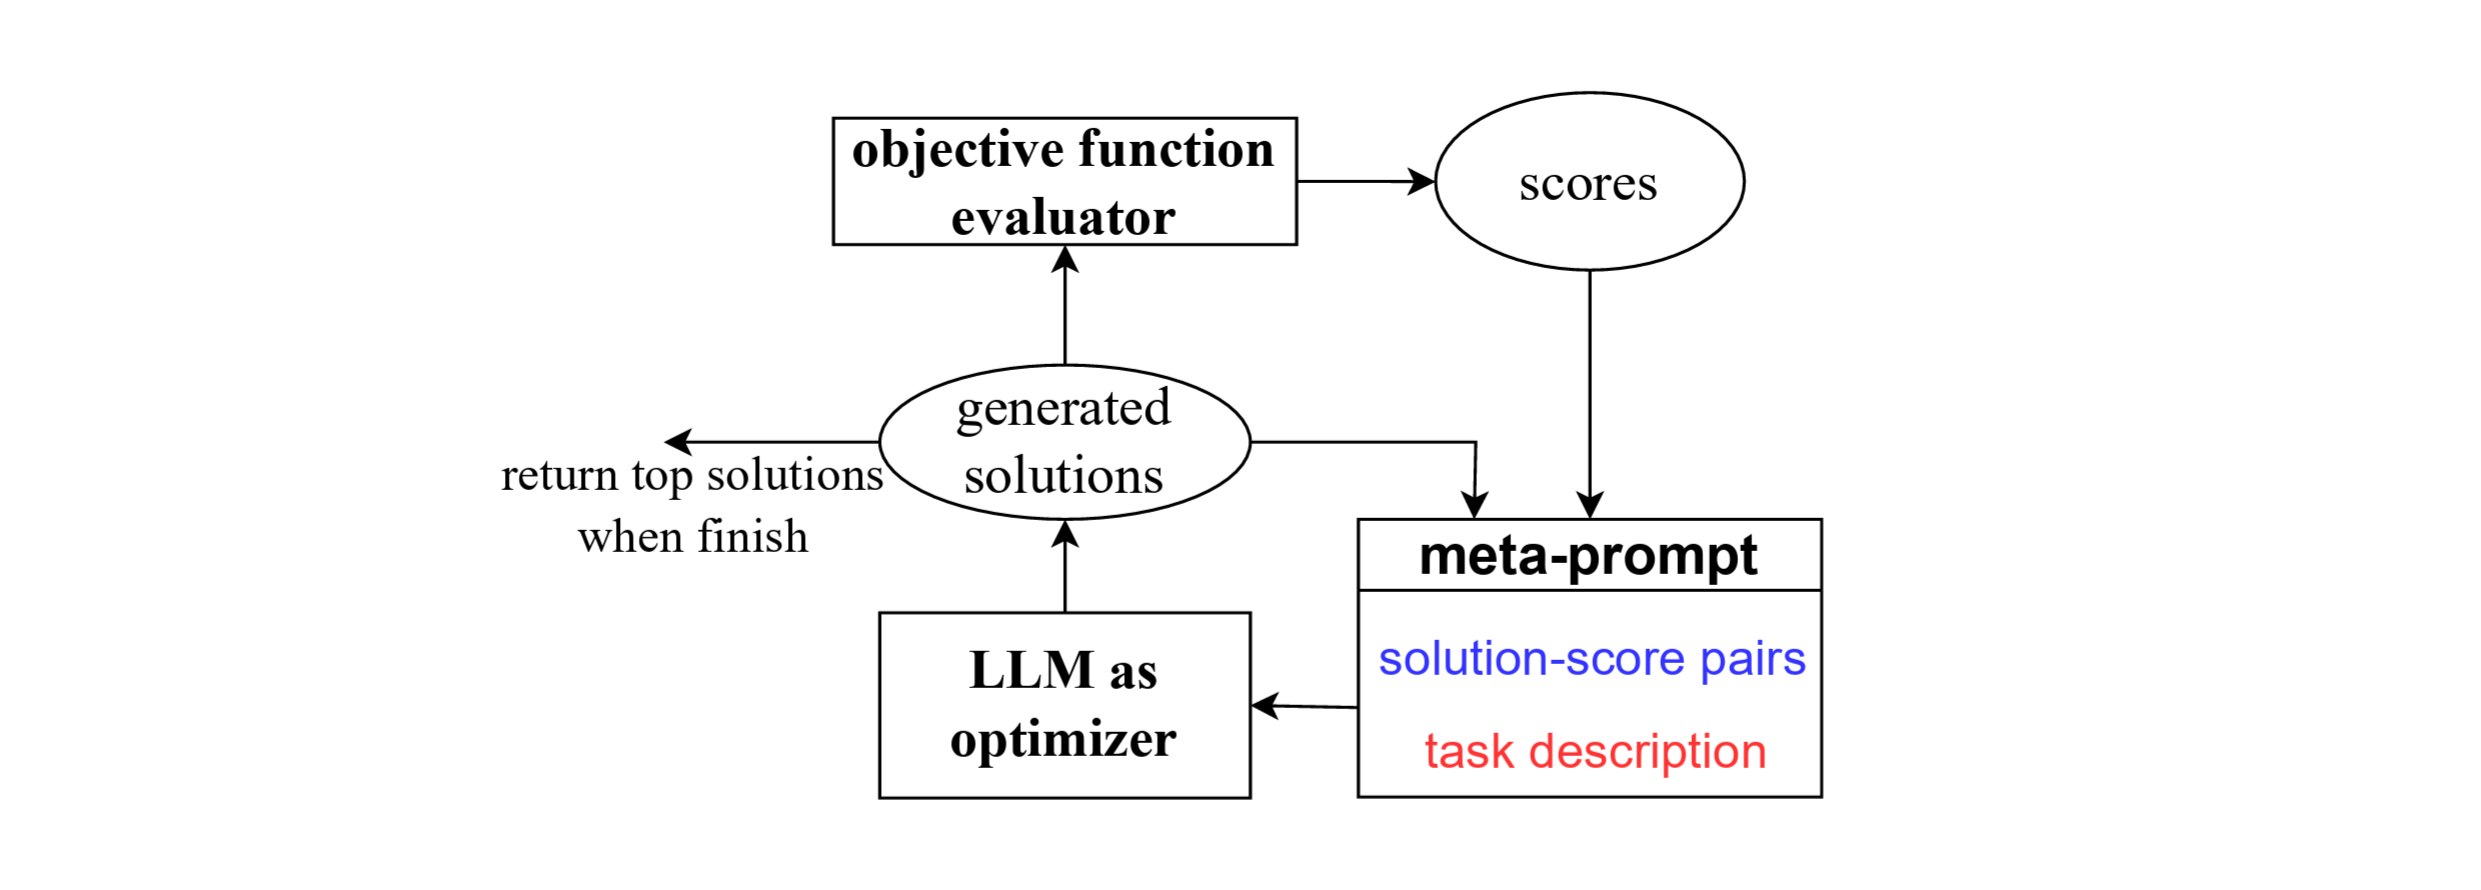
\includegraphics[width=140mm]{images/opro}
	\caption{دیاگرام روش بهینه سازی با اعلان}
	\label{fig_opro}
\end{figure}


از مزایای استفاده از مدل‌های زبانی بزرگ به‌عنوان بهینه‌ساز می\/توان به موارد زیر اشاره کرد:

\begin{itemize}
	\item 
	مدل‌های زبانی بزرگ به دلیل توانایی درک و تولید متنی مشابه انسان، می‌توانند به انواع مختلف مسائل بهینه‌سازی که با زبان طبیعی توصیف می‌شوند، پاسخ دهند.
	\item 
	همچنین این مدل ها قادر به انجام بهینه‌سازی در مسائلی هستند که اطلاعات گرادیان در دسترس نیست یا به‌دست‌آوردن آن دشوار است و به همین دلیل رویکردی بدون نیاز به مشتق ارائه می‌دهند.
	\item 
	از طرفی این مدل ها می‌توانند اعلان‌های خود را بهینه کنند و بدون نیاز به آموزش مجدد، عملکرد خود را در وظایف خاص بهبود دهند.
\end{itemize}




\subsection{روش برنامه\/ریزی و حل}
روش برنامه\/ریزی و حل
\LTRfootnote{Plan-and-Solve (PS)}
یک تکنیک پیشرفته در مهندسی اعلان است که بهبود عملکرد مدل‌های زبانی بزرگ را در حل مسائل پیچیده مورد هدف قرار می‌دهد. در این روش، مدل ابتدا یک برنامه‌ریزی
\LTRfootnote{Planing}
 انجام داده و سپس بر اساس آن، به حل مسئله
\LTRfootnote{Solve}
  می‌پردازد.  

برخلاف روش‌های سنتی که مدل را مستقیماً درگیر حل مسئله می‌کنند، این روش باعث کاهش نرخ خطا شده و دقت پاسخ‌های مدل را افزایش می‌دهد. روش برنامه ریزی و حل به‌ویژه در مسائلی که نیاز به چندین مرحله استدلالی دارند، مانند حل مسائل ریاضی، تحلیل منطقی و برنامه‌ریزی وظایف، بسیار کارآمد است.  


این روش شامل دو مرحله اصلی است:  

\begin{enumerate}
	\item برنامه‌ریزی 
	\LTRfootnote{Plan Phase}:
	مدل یک برنامه کلی برای حل مسئله ارائه می‌دهد، شامل مراحل موردنیاز برای رسیدن به پاسخ.  
	\item حل مسئله
	\LTRfootnote{Solve Phase}:
	مدل بر اساس برنامه تولیدشده، گام‌به‌گام راه‌حل را پیاده‌سازی کرده و پاسخ نهایی را استخراج می‌کند.  
\end{enumerate}  

این تفکیک دو مرحله‌ای، عملکرد مدل را بهبود می‌بخشد زیرا ابتدا ساختار حل مسئله مشخص شده و سپس محاسبات انجام می‌شود.  
در ادامه یک مسئله و راه حل این روش برای آن مسئله را بررسی می\/کنیم.

مسئله:	سن علی ۳ برابر سن برادرش است. ۴ سال پیش، مجموع سن آن‌ها ۲۰ سال بوده است. سن هر یک را مشخص کنید. 

\begin{enumerate}
	\item اجرای مرحله برنامه‌ریزی:
	\begin{itemize}
		\item تعریف متغیرها: فرض کنیم سن برادر علی را $X$ در نظر بگیریم.  
		\item رابطه کنونی: سن علی برابر با $3X$ است.  
		\item رابطه در گذشته: ۴ سال پیش، سن برادر علی برابر $X-4$ و سن علی برابر $3X-4$ بوده است.  
		\item معادله کلی:  
		\[
		(X - 4) + (3X - 4) = 20
		\]
		\item حل معادله و یافتن مقدار $X$
	\end{itemize} 
	
	\item اجرای مرحله حل:
	\[
	X - 4 + 3X - 4 = 20
	\]  
	\[
	4X - 8 = 20
	\]  
	\[
	4X = 28
	\]  
	\[
	X = 7
	\]  
	در نتیجه :  
	\begin{itemize}
		\item سن برادر علی : $7$ سال  
		\item سن علی : $3 \times 7 = 21$ سال  
	\end{itemize}  
\end{enumerate}

با بررسی این مثال می\/توان متوجه افزایش دقت حل مسائل چند مرحله ای با استفاده از روش برنامه ریزی و حل شد و همچنین عملکرد برنامه ریزی و سپس عمل را مشاهده کرد که مشابه سیستم تفکر انسانی است.
در شکل \ref{fig_ps} یک مثال دیگر از این روش آورده شده است.

\begin{figure}[!t]
	\centering
	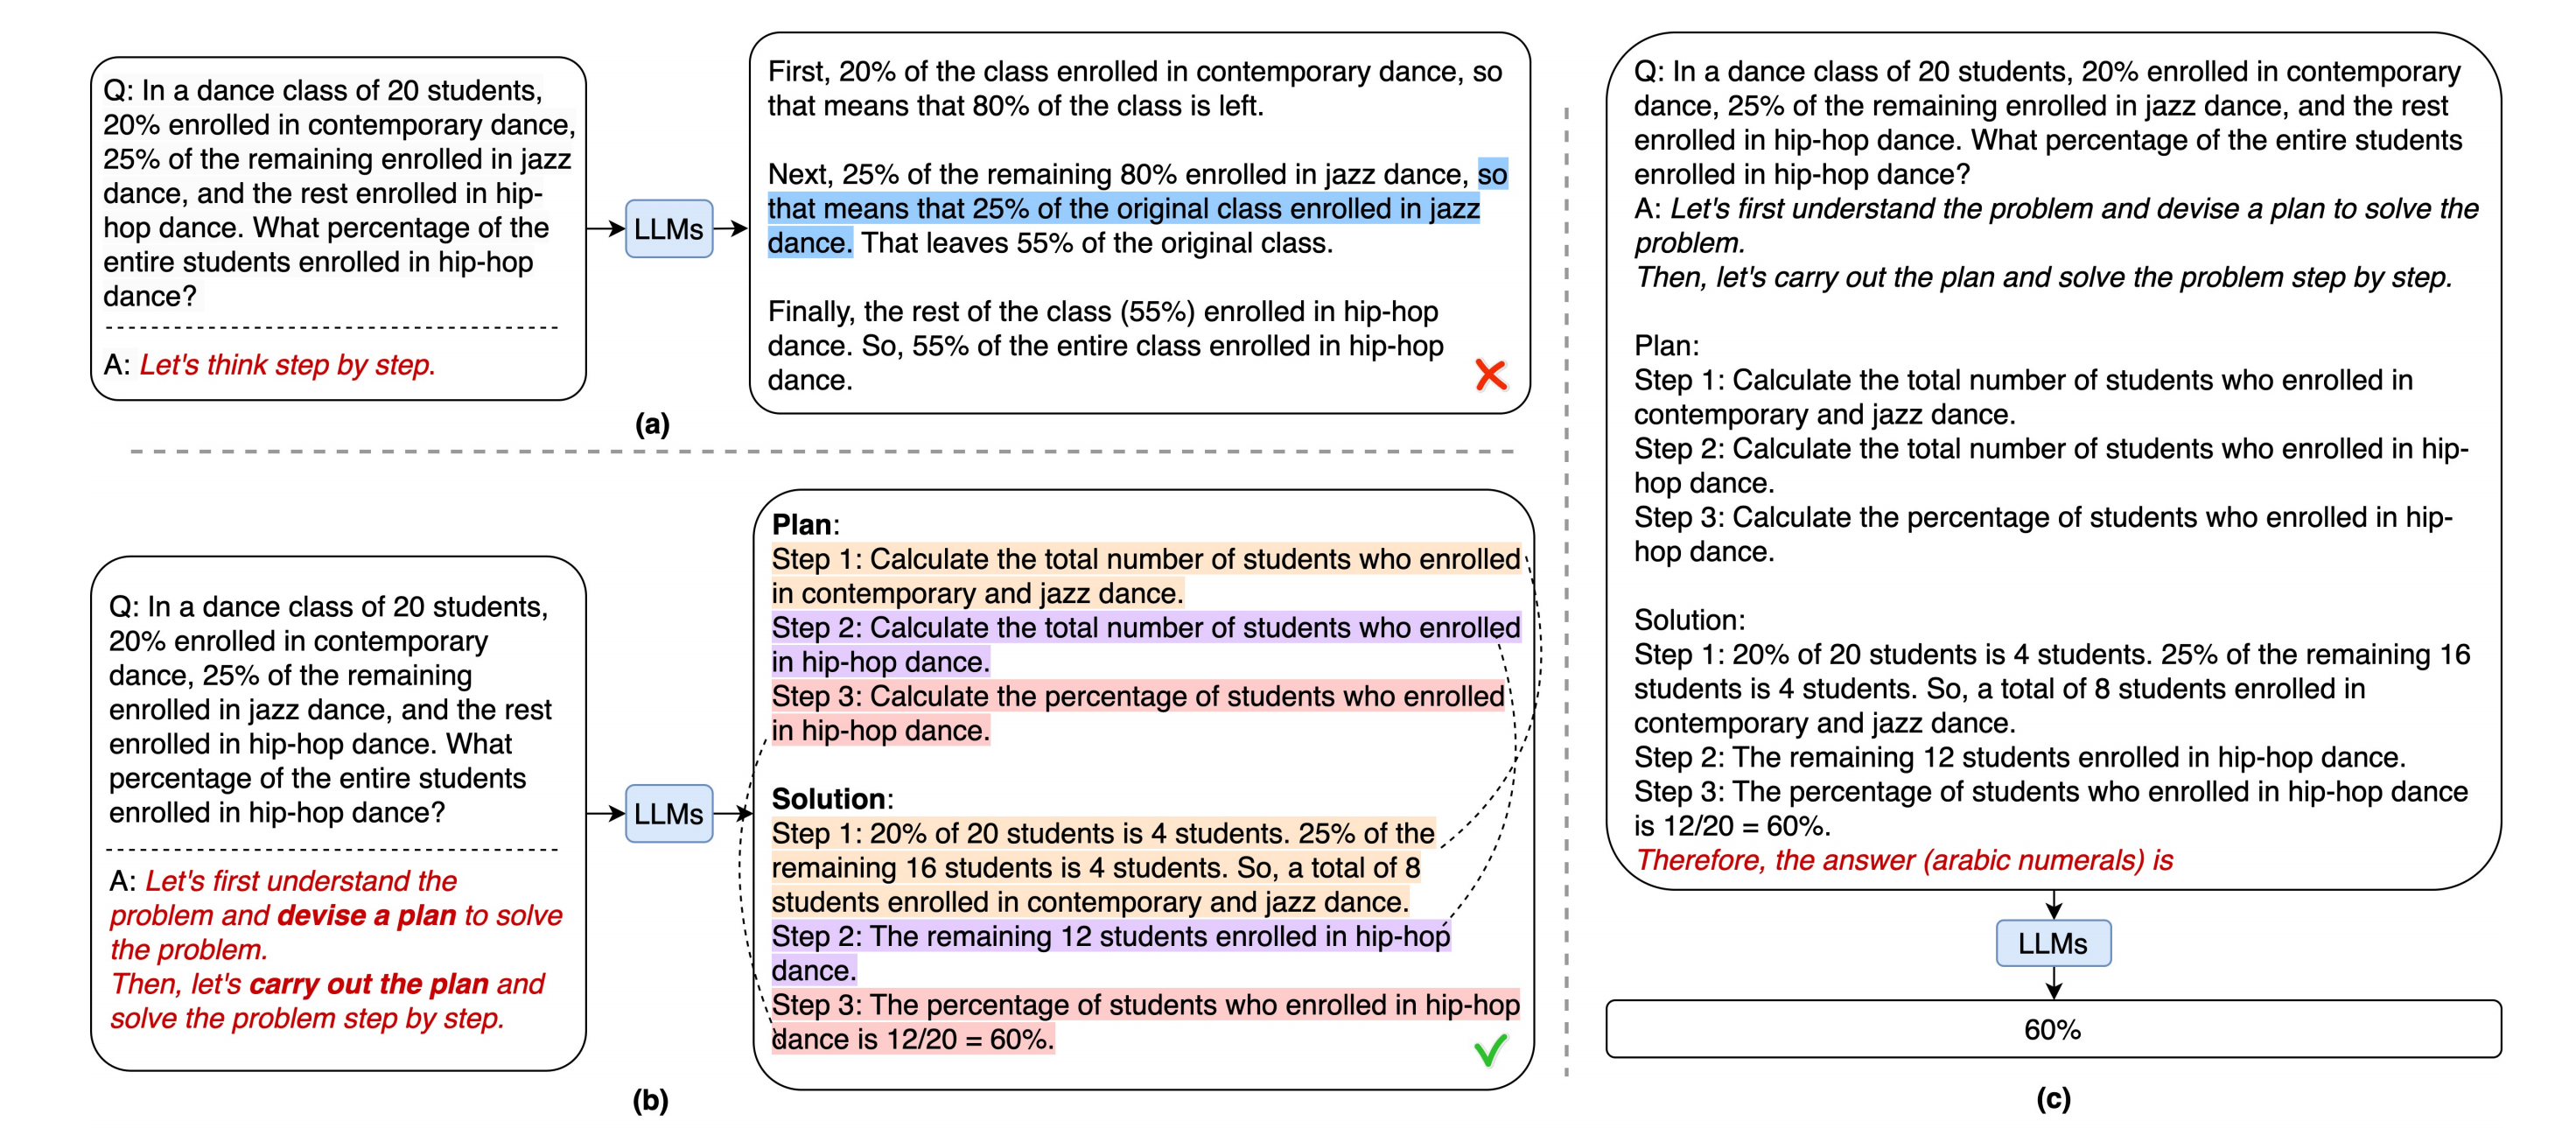
\includegraphics[width=160mm]{images/ps}
	\caption{یک مثال از روش برنامه\/ریزی و حل}
	\label{fig_ps}
\end{figure}


\section{بهینه‌سازی خودکار اعلان‌ها}
بهینه‌سازی خودکار اعلان‌ها یک رویکرد نوین در مهندسی اعلان است که با بهره‌گیری از الگوریتم‌های جستجو و بهینه‌سازی، به صورت سیستماتیک بهترین ورودی‌های متنی را برای مدل‌های زبانی شناسایی و تولید می‌کند. در این روش به جای تکیه بر شهود انسانی و روش‌های آزمون و خطا، از تکنیک‌هایی مانند الگوریتم‌های تکاملی، جستجوی تصادفی و یادگیری تقویتی استفاده می‌شود. این الگوریتم‌ها فضای اعلان‌ها را مورد بررسی قرار داده و بر اساس معیارهای مشخصی مانند دقت، انسجام و ارتباط معنایی، به انتخاب بهینه‌ترین اعلان‌ها می‌پردازند.

یکی از مزایای مهم بهینه‌سازی خودکار اعلان‌ها این است که در مقیاس‌های بزرگ و در زمان‌های کوتاه، قادر به دستیابی به نتایج بهینه می‌باشد. بهینه‌سازی خودکار پرامت ها با ارائه چارچوبی سیستماتیک، امکان ارزیابی سریع و انتخاب اعلان‌های بهینه را فراهم می‌آورد. این دو رویکرد می‌توانند مکمل یکدیگر عمل کرده و در کاربردهایی که نیاز به سرعت و دقت بالا دارند، مانند پردازش دسته‌جمعی داده‌های متنی یا تنظیم خودکار اعلان‌ها برای وظایف متنوع، عملکرد بهتری ارائه دهند.

\subsection{روش زنجیره تفکر خودکار}
از اولین جرقه های خودکارسازی مهندسی اعلان، میتوان به خودکارسازی تولید زنجیره‌های استدلالی در روش زنجیره تفکر اشاره کرد. روش زنجیره تفکر خودکار 
\LTRfootnote{AUTOMATIC CHAIN-OF-THOUGHT PROMPTING (Auto-CoT)} \cite{auto_cot}
 به‌طور خودکار زنجیره‌هایی از استدلال‌ها و سوالات را برای ساخت نسخهها ایجاد می‌کند. این روش شامل دو مرحله اصلی است. مرحله اول خوشه‌بندی سوالات و تقسیم سوالات یک مجموعه‌داده به چندین خوشه و مرحله دوم نمونه‌گیری از نسخهها و انتخاب یک سوال نماینده از هر خوشه و تولید زنجیره استدلال برای آن است. روند کلی این روش در شکل \ref{fig_autocot} نشان داده شده است.

در مرحله اول، از آنجایی که خوشه‌بندی مبتنی بر تنوع می‌تواند از گمراهی ناشی از شباهت جلوگیری کند، این روش تحلیل خوشه‌ای را برای مجموعه‌ای از سوالات $Q$ انجام می‌دهد. بدین صورت که ابتدا برای هر سوال در $Q$، یک بردار نمایشی با استفاده از \lr{Sentence-BERT} \cite{sentenceBert} محاسبه می\/شود و سپس این بردارهای متنی میانگین‌گیری شده و یک بردار با اندازه ثابت برای هر سوال ایجاد می‌شود. پس از آن، با استفاده از الگوریتم خوشه‌بندی k-means ، سوالات به $k$ خوشه تقسیم می‌شوند. در نهایت برای هر خوشه $i$، سوالات آن خوشه را به‌صورت یک لیست مرتب‌شده \lr{$q^{(i)} = [q^{(i)}_1, q^{(i)}_2, \ldots]$} بر اساس فاصله از مرکز خوشه به ترتیب صعودی مرتب می‌شوند.

در مرحله دوم، برای سوالات نمونه‌گیری‌شده، زنجیره‌های استدلال تولید می\/شوند و نسخههایی که با معیارهای انتخاب مطابقت دارند استخراج می\/شوند. به‌طور دقیق‌تر، برای هر خوشه $i$، یک نسخه به صورت \lr{$d^{(i)}$} (ترکیبی از سوال، استدلال و پاسخ) ساخته می\/شود. برای خوشه $i$، سوالات مرتب‌شده در لیست \lr{$q^{(i)} = [q^{(i)}_1, q^{(i)}_2, \ldots]$} تا زمانی که معیارهای انتخاب برآورده شوند، بررسی می‌شوند.

به عبارت دیگر، سوالی که به مرکز خوشه نزدیک‌تر است، زودتر بررسی می‌شود. فرض کنید سوال \lr{$q^{(i)}_j$} که $j$-اُمین سوال نزدیک به مرکز خوشه $i$ است، در حال بررسی باشد. یک ورودی به شکل زیر ساخته می‌شود:

\begin{center}
	\lr{[Q: $q^{(i)}_j$ A: [P]]}
\end{center}

سپس یک نسخه کاندید برای خوشه $i$ به صورت زیر ساخته می‌شود:

\begin{center}
	\lr{[Q: $q^{(i)}_j$ A: $r^{(i)}_j$ $a^{(i)}_j$]}
\end{center}

مشابه معیارهای مورد استفاده در نسخه\/های دستی روش زنجیره تفکر \cite{CoT}, معیار انتخاب این الگوریتم نیز بر قوانین ساده‌ای تکیه دارد تا سوالات و استدلال‌های ساده‌تر را انتخاب کند: نسخه \lr{$d^{(i)}$} به‌عنوان \lr{$d^{(i)}_j$} انتخاب می‌شود اگر سوال \lr{$q^{(i)}_j$} دارای کمتر از ۶۰ توکن و استدلال \lr{$r^{(i)}_j$} دارای کمتر از ۵ گام استدلالی باشد.

\begin{figure}[!t]
	\centering
	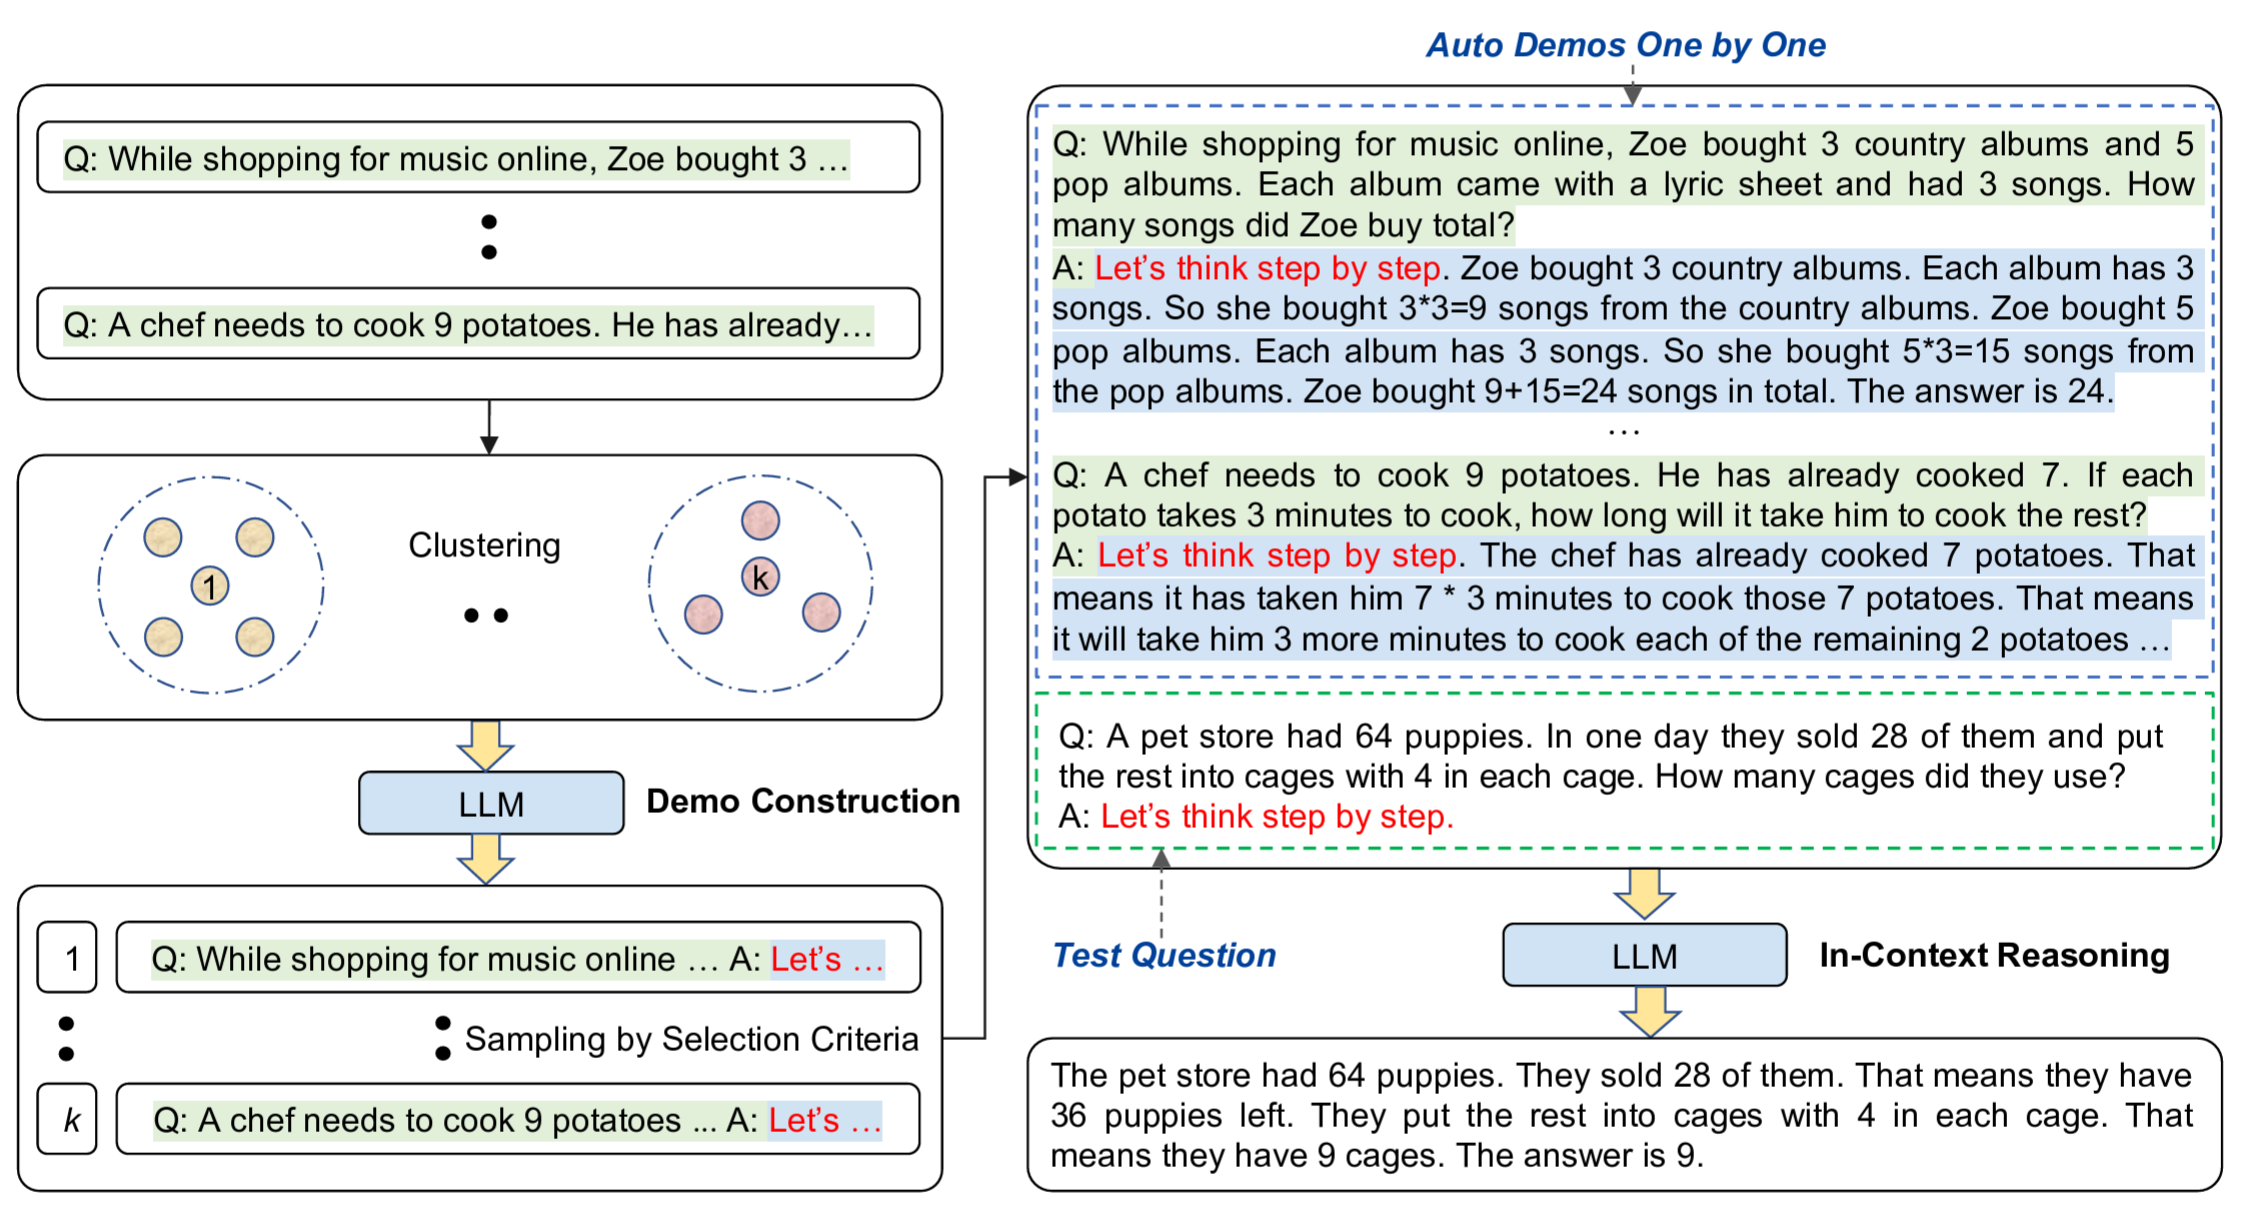
\includegraphics[width=140mm]{images/autocot}
	\caption{دیاگرام روش auto-CoT}
	\label{fig_autocot}
\end{figure}

\subsection{روش مهندس اعلان خودکار}
روش  مهندس اعلان خودکار
\LTRfootnote{Auto Prompt Engineer} \cite{APE}
 از خود مدل‌های زبانی بزرگ برای خودکارسازی فرآیند ایجاد و بهینه‌سازی اعلان‌ها استفاده می‌کند. در این روش، یک مدل زبانی، مجموعه‌ای از اعلان‌های مختلف تولید می‌کند و سپس این اعلان‌ها بر اساس کیفیت پاسخ‌هایی که از یک مدل دیگر دریافت می‌شود، ارزیابی می‌شوند. این فرآیند به‌صورت تکراری ادامه می‌یابد تا مؤثرترین اعلان‌ها شناسایی شوند. نتایج در ۲۴ وظیفه مختلف در حوزه پردازش زبان طبیعی نشان داده که اعلان‌های تولید شده توسط این روش در اغلب موارد عملکرد بهتری نسبت به روش‌های قبلی داشته‌اند و در ۱۹ مورد از ۲۴ وظیفه، کیفیتی معادل یا نزدیک به اعلان‌های طراحی شده توسط انسان ارائه کرده‌اند.

تأثیرات این روش قابل توجه است؛ این روش نیاز به مهندسان اعلان انسانی را کاهش می‌دهد، فرآیند توسعه را سریع‌تر می‌کند و سازگاری مدل‌های زبانی بزرگ با وظایف مختلف را افزایش می‌دهد. این پیشرفت نشان‌دهنده ظرفیت مدل‌های بزرگ زبانی برای نه‌تنها انجام وظایف، بلکه بهینه‌سازی دستورالعمل‌های خودشان نیز هست و گامی مهم به سوی سامانه‌های هوشمند خودمختارتر به‌شمار می‌رود.

\subsection{روش مولد اعلان}
روش مولد اعلان
\LTRfootnote{Promptbreeder} \cite{PromptBreeder}
 یک سیستم خودارجاعی
 \LTRfootnote{self-referential}
  و تکاملی برای بهبود خودکار اعلان‌های مورد استفاده در مدل‌های زبانی بزرگ است. این روش با الهام از الگوریتم‌های تکاملی و فرآیندهای خودبهبوددهی
  \LTRfootnote{self-improvment}
  ، به جای اتکا بر اعلان‌های دستی و مهندسی‌شده، به طور خودکار اعلان‌هایی را تولید و اصلاح می‌کند که می‌توانند عملکرد مدل را در حل مسائل مختلف بهبود بخشند. ویژگی کلیدی این روش این است که نه‌تنها اعلان‌های وظیفه
  \LTRfootnote{Task Prompts}
   را تکامل می‌دهد، بلکه اعلان‌های تغییر
   \LTRfootnote{Mutation Prompts}
    را نیز که برای تغییر اعلان‌های مورد جستجو استفاده می‌شوند، بهبود می‌بخشد.  

این الگوریتم از یک فرآیند تکاملی مبتنی بر جمعیت
\LTRfootnote{population base}
 استفاده می‌کند. همانطور که در شکل \ref{fig_promptbreeder} نشان داده شده است، در ابتدا یک مجموعه از اعلان‌های اولیه به همراه دستورات تغییر تولید می‌شود. سپس، در هر نسل از فرآیند تکامل: 
 \begin{enumerate}
 	\item ارزیابی سازگاری
 	\LTRfootnote{Fitness Evaluation}: اعلان‌ها بر اساس عملکردشان در پاسخ‌دهی به مجموعه‌ای از سؤالات آموزشی ارزیابی می‌شوند.
 	
 	\item انتخاب
 	\LTRfootnote{Selection}: دو اعلان به‌صورت تصادفی انتخاب شده و مقایسه می‌شوند؛ اعلانی که عملکرد بهتری داشته باشد، انتخاب می‌شود.
 	
 	\item اعمال تغییرات
 	\LTRfootnote{Mutation}: اعلان انتخاب‌شده با استفاده از عملگرهای تکاملی تغییر داده می‌شود. این تغییرات شامل تولید نسخه‌های جدید از اعلان، اصلاح بر اساس الگوهای موفق، و یا حتی بهبود خود دستور تغییر است.  
 	
 	\item جایگزینی
 	\LTRfootnote{Replacement}: نسخه‌ی بهبودیافته جایگزین اعلان با عملکرد ضعیف‌تر شده و این فرآیند در نسل‌های بعدی تکرار می‌شود.
 \end{enumerate} 

عملگرهای تکاملی شامل جهش مستقیم
\LTRfootnote{Direct Mutation}
، جهش مبتنی بر توزیع
\LTRfootnote{Estimation of Distribution (EDA) Mutation}
، ابرجهش
\LTRfootnote{Hypermutation}
، جهش لامارکین
\LTRfootnote{Lamarckian Mutation}
، و ترکیب اعلان‌ها
\LTRfootnote{Prompt Crossover and Context Shuffling}
 هستند که هر یک روش‌های متفاوتی را برای اصلاح و بهبود اعلان‌ها ارائه می‌دهند. با ادامه این فرآیند در طی چندین نسل، اعلان‌ها به تدریج بهینه شده و به عملکرد بهتری در مدل‌های زبانی منجر می‌شوند.  
 
\begin{figure}[!t]
	\centering
	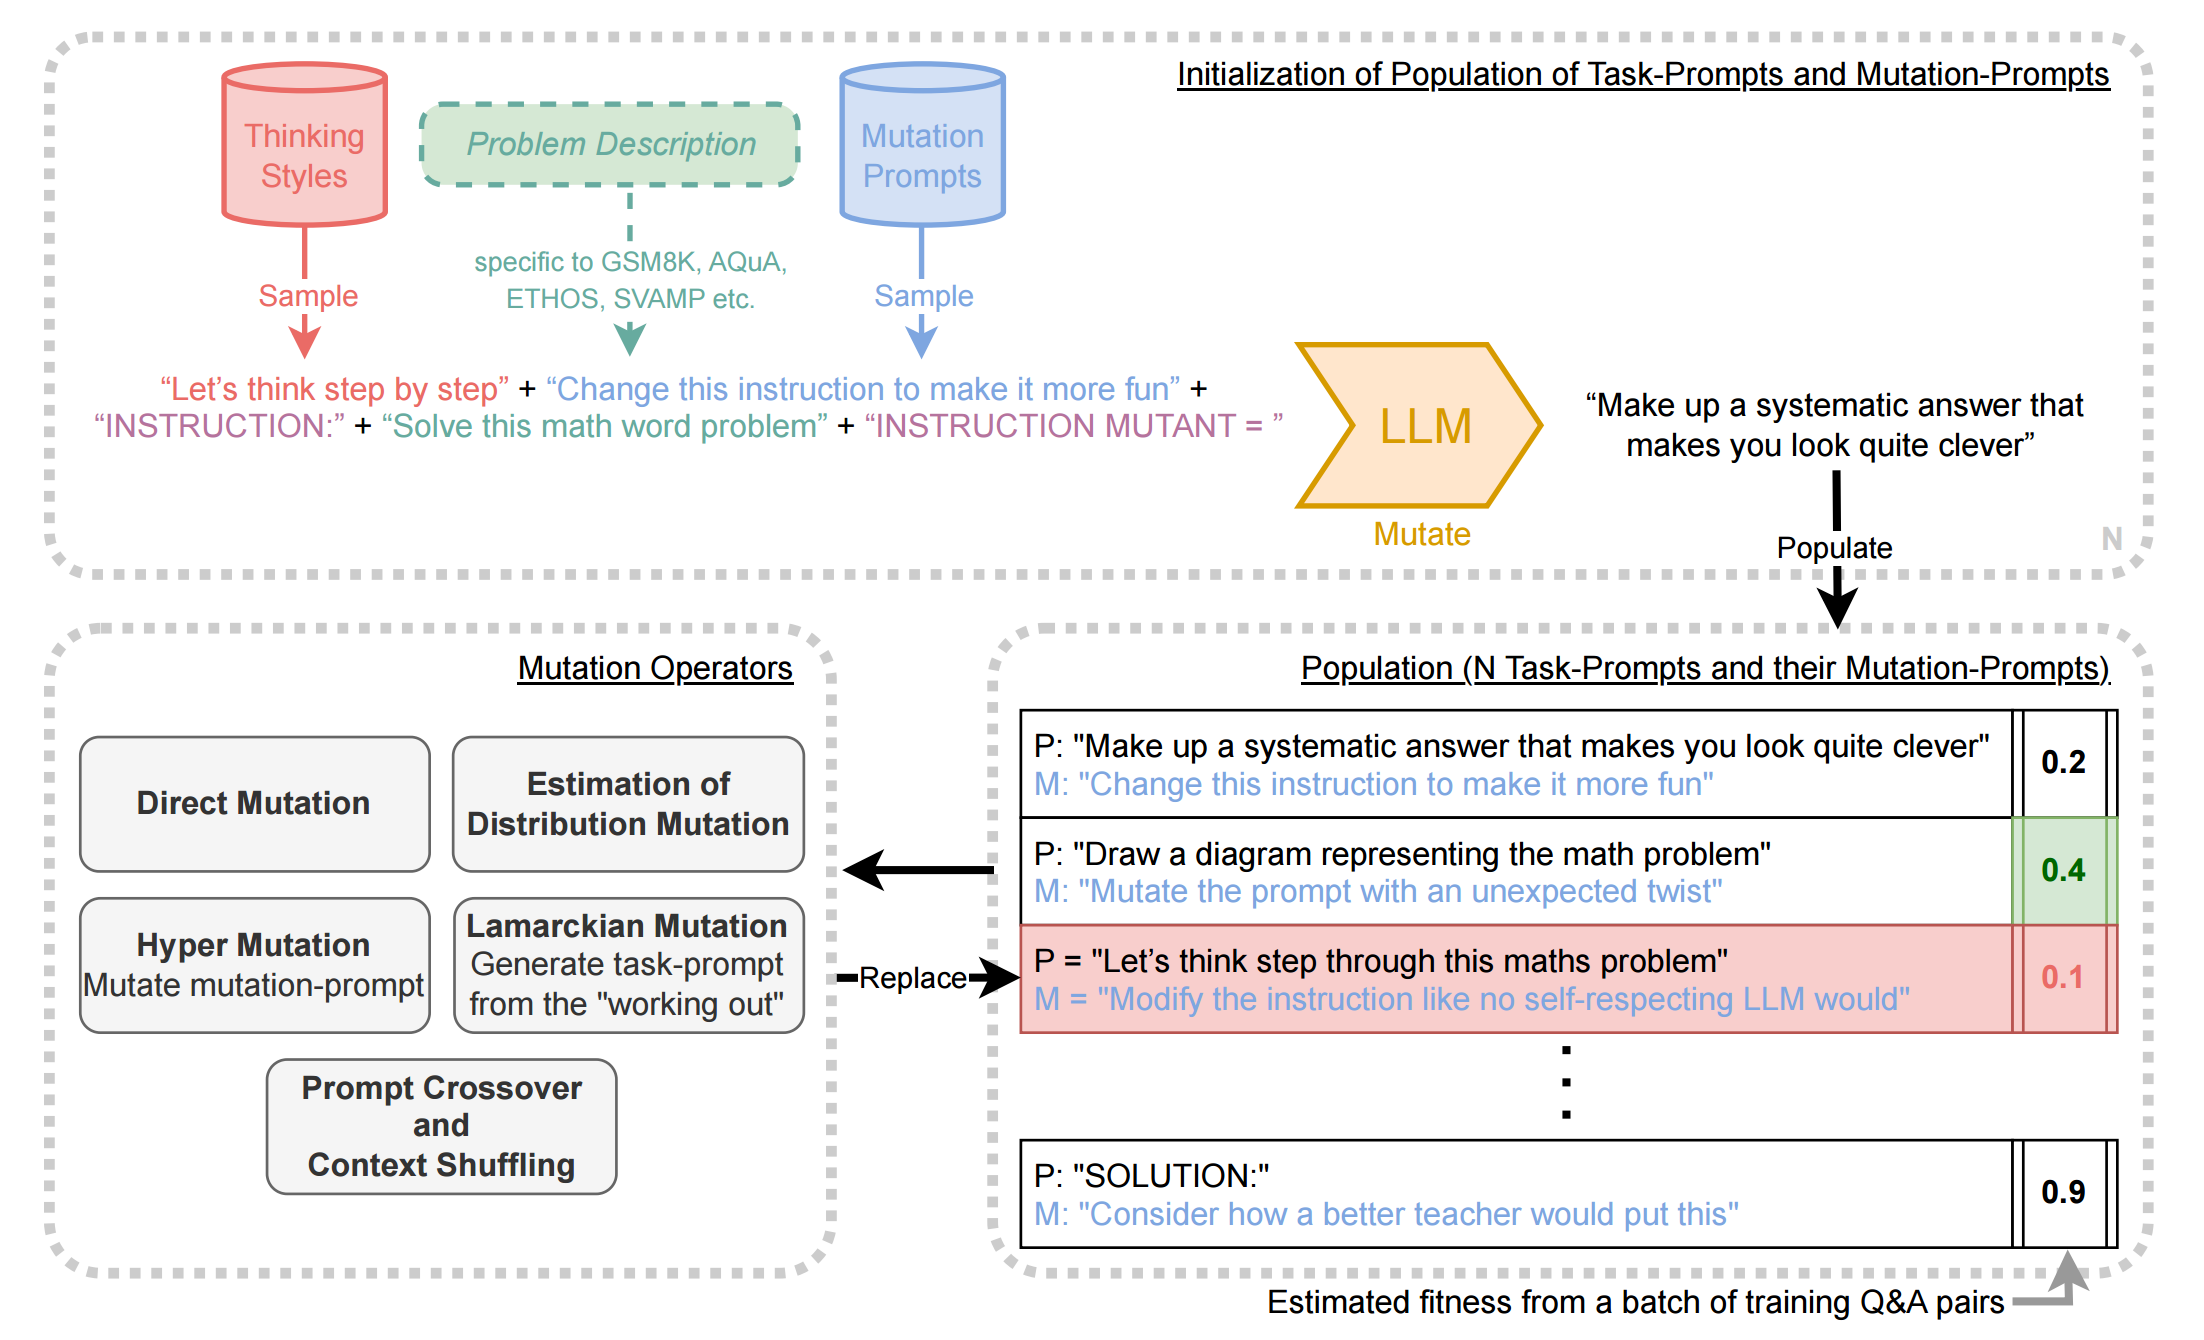
\includegraphics[width=140mm]{images/promptbreeder}
	\caption{دیاگرام روش مولد اعلان}
	\label{fig_promptbreeder}
\end{figure}

روش مولد اعلان در آزمایش‌های مختلف نشان داده است که می‌تواند از روش‌های متداول مهندسی اعلان مانند CoT و PS عملکرد بهتری داشته باشد. همچنین، این سیستم در حوزه‌های مختلف مانند حل مسائل ریاضی، استدلال عمومی
\LTRfootnote{commonsense reasoning}
، و کلاس‌بندی گفتار نفرت‌آمیز
\LTRfootnote{hate speech classification}
 بهبود چشمگیری ایجاد کرده است. مهم‌ترین مزیت آن این است که به به‌روزرسانی پارامترهای مدل نیازی ندارد و تنها از طریق اصلاح اعلان‌ها، کارایی مدل را افزایش می‌دهد.  

این روش نشان‌دهنده‌ی قدرت بهینه‌سازی خودکار اعلان‌ها و حرکت به‌سوی سیستم‌های هوش مصنوعی خودبهبوددهنده و خودارجاعی است که می‌توانند با حداقل مداخله انسانی، عملکرد خود را در طی زمان بهبود بخشند.


\section{جمع‌بندی مباحث ارائه‌شده}
این فصل با هدف بررسی پیشینه تحقیق و تبیین مفاهیم بنیادی مرتبط با موضوع پژوهش تدوین گردید. در این فصل، تلاش شد تا ضمن ارائه چارچوب نظری جامع، زمینه مناسبی برای درک بهتر مسأله تحقیق و مسیر پژوهش فراهم شود. با توجه به گستره و عمق موضوعات مطرح‌شده، می‌توان این فصل را به‌عنوان شالوده‌ای برای تحلیل‌ها و مطالعات تخصصی‌تر در فصول بعدی قلمداد نمود.

در این فصل، نخست به معرفی و تحلیل مدل‌های زبان بزرگ پرداخته شد و روند تکاملی این مدل‌ها از آغاز تا وضعیت کنونی آن‌ها مورد بررسی قرار گرفت. در ادامه، به معماری‌های رایج و کاربردهای متنوع این مدل‌ها اشاره شد و اهمیت آن‌ها در پیشبرد حوزه‌های مختلف پردازش زبان طبیعی و سامانه‌های مبتنی بر هوش مصنوعی تبیین گردید.

سپس، به موضوع مهندسی اعلان و نقش آن در بهره‌برداری مؤثر از مدل‌های زبان بزرگ پرداخته شد. در این بخش، ابتدا روش‌های سنتی مهندسی اعلان، شامل استفاده از یادگیری درون متنی، روش زنجیره تفکر ، استدلال بدون نمونه آموزشی، برنامه تفکر، بهینه سازی با اعلان و روش برنامه\/ریزی و حل به تفصیل بررسی شدند. در ادامه، به معرفی و تحلیل رویکردهای نوین در بهینه‌سازی خودکار اعلان‌ها پرداخته شد. از جمله این روش‌ها می‌توان به زنجیره تفکر خودکار، مهندسی اعلان خودکار و روش مولد اعلان اشاره نمود که هریک با هدف افزایش دقت و توان استدلال مدل‌های زبانی توسعه یافته‌اند.


بر مبنای مباحث ارائه‌شده، آشکار شد که مهندسی اعلان و بهینه‌سازی آن از مهم‌ترین مؤلفه‌ها در افزایش کارایی مدل‌های زبان بزرگ به شمار می‌رود. این امر اهمیت طراحی الگوریتم‌های نوین و کارآمد برای بهبود ساختار و محتوای اعلان‌ها را دوچندان می‌سازد.

در فصل آتی، به تشریح کامل الگوریتم پیشنهادی پرداخته خواهد شد. این الگوریتم که مولد اعلان ساده نام دارد، یکی از رویکردهای نوین در زمینه بهینه‌سازی و تکامل خودکار اعلان‌ها محسوب می‌شود و مبتنی بر اصول الگوریتم‌های تکاملی و بهبود مستمر اعلان‌ها از طریق تولید، ارزیابی و گزینش نسل‌های مختلف اعلان‌ها طراحی شده است. در فصل آینده، به‌طور دقیق به ساختار، مراحل اجرایی و مزایای این الگوریتم در مقایسه با سایر روش‌ها پرداخته خواهد شد.
%فصل دوم
\cleardoublepage
\captionsetup[figure]{labelfont={bf},name={شکل},labelsep=period}
\captionsetup[algorithm]{labelfont={bf},name={الگوریتم},labelsep=period}
\clearpage
\thispagestyle{empty}
\chapter{روش پیشنهادی}\label{chap3}

\section{روش پیشنهادی}

با توجه به رشد روزافزون استفاده از سیستم‌عامل اندروید \citep{Statista2024} و در نتیجه، افزایش تهدیدات بدافزاری متوجه این پلتفرم \citep{Faruki2015, AndroidSecurity}, نیاز به روش‌های کارآمد و دقیق برای شناسایی بدافزارها بیش از پیش احساس می‌شود. این فصل به تشریح دقیق روش پیشنهادی این پژوهش، موسوم به \textbf{MAGNET} (تحلیل چندوجهی برای شناسایی تهدیدات مبتنی بر گراف و شبکه)، اختصاص دارد. این رویکرد با بهره‌گیری از داده‌های چندوجهی—جدولی، گرافی و ترتیبی—و ترکیب آن با معماری‌های پیشرفته یادگیری عمیق از جمله ترنسفورمرها و شبکه‌های عصبی گرافی (GNN)، محدودیت‌های روش‌های تحلیل ایستا و پویا را برطرف می‌کند. هدف اصلی، افزایش دقت شناسایی و تعمیم‌پذیری، به‌ویژه در مواجهه با تهدیدات روز صفر (Zero-Day) است. این بخش به صورت زیر سازمان‌دهی شده است: مقدمه‌ای بر روش پیشنهادی، فرضیات و ابزارهای محاسباتی، روش‌شناسی دقیق (شامل پیش‌پردازش داده‌ها، طراحی مدل، آموزش، بهینه‌سازی ابرپارامترها و ارزیابی) و جمع‌بندی نهایی. تمامی فرضیات، ابزارها، معادلات و شبه‌کدها به طور کامل مستند شده‌اند تا امکان تکرارپذیری فراهم باشد.

\subsection{مقدمه روش پیشنهادی}

شناسایی بدافزار اندروید با چالش‌های مهمی روبروست که ناشی از محدودیت‌های رویکردهای سنتی است. روش‌های تحلیل ایستا، مانند بررسی کد منبع یا تحلیل مجوزها، اغلب در شناسایی بدافزارهای پیچیده که از تکنیک‌های مبهم‌سازی یا رمزنگاری استفاده می‌کنند، ناکام می‌مانند \cite{Drebin}. این روش‌ها قادر به ثبت رفتارهای زمان اجرا یا سازگاری‌های پویا در برنامه‌های مخرب نیستند. در مقابل، تحلیل پویا که رفتار برنامه را در حین اجرا پایش می‌کند، محاسبات سنگینی دارد، زمان‌بر است و به دلیل عدم پوشش کامل مسیرهای اجرایی، پوشش کد ناقصی ارائه می‌دهد. این کاستی‌ها به‌ویژه در مواجهه با بدافزارهای روز صفر—تهدیداتی با الگوهای ناشناخته که از سیستم‌های مبتنی بر امضا یا قوانین فرار می‌کنند—بیشتر مشهود است.

برای غلبه بر این چالش‌ها، ما ادغام داده‌های چندوجهی را پیشنهاد می‌کنیم تا دیدی جامع از ویژگی‌های برنامه ارائه شود. به طور خاص، از داده‌های زیر استفاده شده است:
\begin{itemize}
    \item \textbf{داده‌های جدولی}: ویژگی‌های ایستا مانند مجوزها، تعداد فایل‌ها و اندازه برنامه که بینشی از خصوصیات ساختاری ارائه می‌دهند.
    \item \textbf{داده‌های گرافی}: گراف‌های فراخوانی توابع که روابط ساختاری بین توابع را نمایش می‌دهند و وابستگی‌های داخلی برنامه را ثبت می‌کنند.
    \item \textbf{داده‌های ترتیبی}: توالی‌های فراخوانی API که الگوهای رفتاری زمانی در حین اجرا را منعکس می‌کنند.
\end{itemize}
این رویکرد چندوجهی، استخراج اطلاعات مکمل را تضمین می‌کند و خلأهای تحلیل‌های تک‌وجهی را پر می‌کند. افزون بر این، از معماری‌های پیشرفته یادگیری عمیق—ترنسفورمرها و GNN ها—برای مدل‌سازی الگوهای پیچیده در داخل و بین این وجه‌ها استفاده شده است. ترنسفورمرها در ثبت وابستگی‌های بلندمدت در داده‌های ترتیبی و جدولی برتری دارند، در حالی که GNNها داده‌های گرافی را با بهره‌گیری از روابط گره‌ها و یال‌ها به طور مؤثر پردازش می‌کنند \cite{attention, Kipf2017}.

نوآوری اصلی این پژوهش در مدل \textbf{MAGNET} نهفته است که سه ماژول تخصصی \textit{EnhancedTabTransformer}، \textit{GraphTransformer} و \textit{SequenceTransformer}را با یک مکانیزم توجه پویا و لایه ادغام چندوجهی ترکیب می‌کند. مکانیزم توجه پویا به طور تطبیقی اهمیت ویژگی‌ها را در هر وجه تنظیم می‌کند، در حالی که لایه ادغام، بازنمایی‌های چندوجهی را به یک فضای ویژگی منسجم برای طبقه‌بندی تبدیل می‌کند. این طراحی، دقت شناسایی، پایداری و تطبیق‌پذیری در برابر تهدیدات در حال تحول را بهبود می‌بخشد و MAGNET را به پیشرفتی چشمگیر نسبت به روش‌های موجود تبدیل می‌کند.

\subsection{فرضیات و ابزارهای محاسباتی}

\subsubsection{فرضیات}
طراحی و ارزیابی MAGNET بر اساس فرضیات زیر استوار است:
\begin{enumerate}
    \item \textbf{ماهیت مکمل داده‌های چندوجهی}: ترکیب داده‌های جدولی، گرافی و ترتیبی، بازنمایی جامع‌تری از رفتار بدافزار ارائه می‌دهد و عملکرد شناسایی را بهبود می‌بخشد.
    \item \textbf{مناسب بودن معماری‌های پیشرفته}: ترنسفورمرها و GNNها برای استخراج الگوهای پیچیده از داده‌های ساختاریافته و ترتیبی مناسب هستند.
    \item \textbf{کارایی توجه پویا}: مکانیزم توجه پویا با اختصاص وزن‌های آگاه از زمینه به ویژگی‌ها، عملکرد مدل را ارتقا می‌دهد.
    \item \textbf{بهینه‌سازی مؤثر}: استفاده از بهینه‌ساز Adam برای به‌روزرسانی وزن‌ها و Optuna برای تنظیم ابرپارامترها، همگرایی کارآمد و پیکربندی بهینه مدل را تضمین می‌کند.
\end{enumerate}

\subsubsection{ابزارهای محاسباتی}
پیاده‌سازی و ارزیابی MAGNET با استفاده از ابزارها و منابع زیر انجام شد:
\begin{itemize}
    \item \textbf{زبان برنامه‌نویسی}: \lr{Python 3.8.5}، به دلیل اکوسیستم گسترده محاسبات علمی.
    \item \textbf{کتابخانه‌ها}:
        \begin{itemize}
            \item \lr{PyTorch 1.9.0}: برای ساخت و آموزش مدل‌های یادگیری عمیق.
            \item \lr{PyTorch Geometric 1.7.0}: برای پردازش داده‌های گرافی.
            \item \lr{Scikit-learn 0.24.2}: برای محاسبه معیارهای ارزیابی.
            \item \lr{Optuna 2.10.0}: برای بهینه‌سازی ابرپارامترها.
        \end{itemize}
    \item \textbf{سخت‌افزار}:
        \begin{itemize}
            \item \lr{GPU: NVIDIA RTX 3090} با ۲۴ گیگابایت \lr{VRAM} و ۱۰٬۴۹۶ هسته \lr{CUDA}، برای محاسبات موازی کارآمد.
            \item \lr{CPU: Intel Xeon E5-2690 v4} با ۳۲ هسته و فرکانس ۲.۶ گیگاهرتز، برای پشتیبانی از پیش‌پردازش و بهینه‌سازی.
            \item \lr{RAM}: ۱۲۸ گیگابایت \lr{DDR4}، برای مدیریت داده‌های مقیاس بزرگ.
        \end{itemize}
    \item \textbf{دیتاست}: دیتاست DREBIN \cite{Drebin}، شامل ۵٬۵۶۰ نمونه بدافزار و ۵٬۰۰۰ نمونه سالم. این دیتاست شامل:
        \begin{itemize}
            \item ویژگی‌های جدولی: مانند تعداد مجوزها (میانگین = \lr{۱۲.۳}، انحراف معیار = \lr{۴.۱})، اندازه فایل (میانگین = \lr{۲.۸} مگابایت، انحراف معیار = \lr{۱.۹} مگابایت).
            \item ویژگی‌های گرافی: گراف‌های فراخوانی توابع با میانگین ۱٬۲۴۵ گره و ۳٬۸۷۲ یال در هر نمونه.
            \item ویژگی‌های ترتیبی: توالی‌های فراخوانی API با میانگین طول ۸۷ فراخوانی در هر نمونه.
        \end{itemize}
\end{itemize}

\subsection{روش‌شناسی}

\subsubsection{پیش‌پردازش داده‌ها}
دیتاست DREBIN برای سازگاری با مدل MAGNET پیش‌پردازش شد. هر وجه به صورت زیر پردازش شد:

\begin{itemize}
    \item \textbf{داده‌های جدولی}:
        \begin{itemize}
            \item \textit{استخراج ویژگی}: ۱۲۸ ویژگی ایستا استخراج شد، مانند تعداد مجوزها، تعداد فایل‌ها و اندازه برنامه، که یک بردار ویژگی \( \mathbf{x}_{\text{tab}} \in \mathbb{R}^{128} \) را تشکیل می‌دهند.
            \item \textit{نرمال‌سازی}: ویژگی‌ها با استفاده از استانداردسازی نرمال‌سازی شدند:
            \[
            x_{\text{norm}} = \frac{x - \mu}{\sigma},
            \]
            که در آن \( \mu \) و \( \sigma \) میانگین و انحراف معیار هر ویژگی در مجموعه آموزش هستند (مثلاً برای مجوزها: \( \mu = 12.3 \)، \( \sigma = 4.1 \)).
        \end{itemize}
    \item \textbf{داده‌های گرافی}:
        \begin{itemize}
            \item \textit{ساخت گراف}: گراف‌های فراخوانی توابع به صورت \( G = (V, E) \) نمایش داده شدند، که در آن \( V \) (گره‌ها) توابع با ویژگی‌های \( \mathbf{x}_v \in \mathbb{R}^{64} \) (مانند نوع تابع، فراوانی) و \( E \) (یال‌ها) فراخوانی‌ها با ویژگی‌های \( \mathbf{e}_{uv} \in \mathbb{R}^{32} \) (مانند فراوانی فراخوانی) هستند.
            \item \textit{فرمت‌بندی}: گراف‌ها به اشیاء \texttt{Data} در PyTorch Geometric تبدیل شدند و ماتریس‌های مجاورت برای کاهش مصرف حافظه، اسپارس‌سازی شدند (میانگین اسپارسیتی = 0.0025).
        \end{itemize}
    \item \textbf{داده‌های ترتیبی}:
        \begin{itemize}
            \item \textit{استخراج توالی}: توالی‌های فراخوانی API به طول ثابت ۱۰۰ کوتاه یا پد شدند، که \( \mathbf{x}_{\text{seq}} \in \mathbb{Z}^{100} \) را تشکیل می‌دهند.
            \item \textit{کدگذاری}: یک واژه‌نامه با ۲٬۱۳۴ فراخوانی API منحصربه‌فرد ساخته شد و توالی‌ها به اعداد صحیح توکنایز شدند (توکن پد = ۰).
        \end{itemize}
\end{itemize}

\subsubsection{طراحی مدل MAGNET}
مدل MAGNET شامل سه ماژول تخصصی برای هر وجه، یک مکانیزم توجه پویا، یک طبقه‌بند باینری است. شکل \ref{fig:magnet_architecture} معماری کلی را نشان می‌دهد.

\begin{figure}[ht]
	\centering
    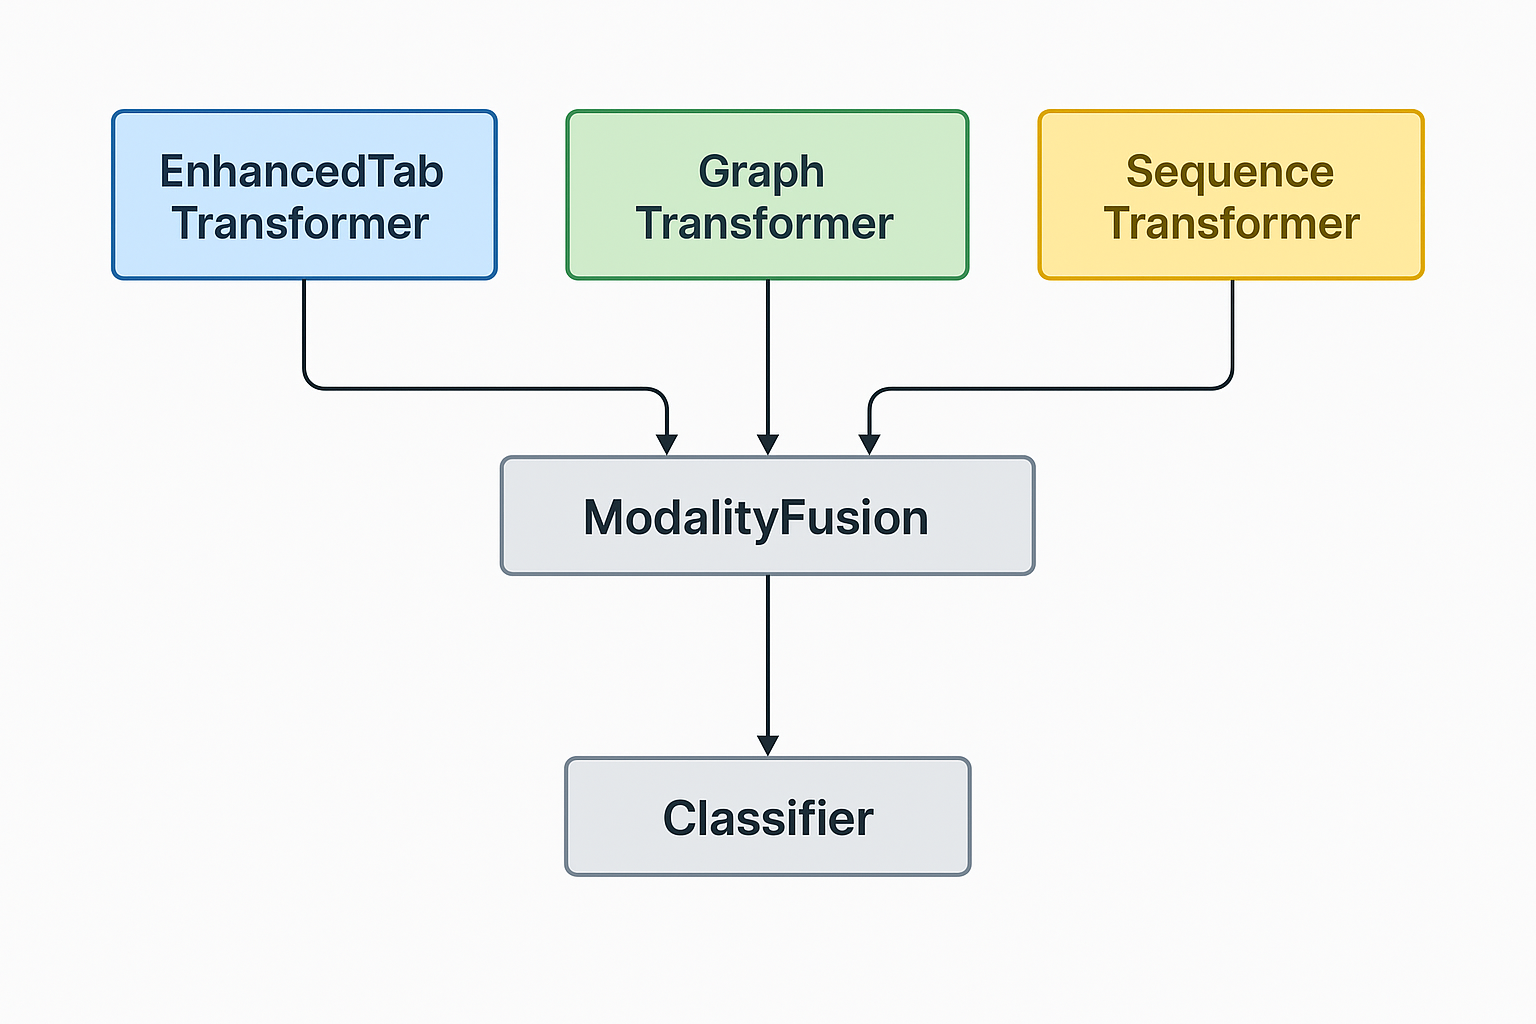
\includegraphics[width=0.9\textwidth]{magnet_architecture}
    \caption{معماری مدل MAGNET شامل سه ماژول تخصصی (EnhancedTabTransformer، GraphTransformer، SequenceTransformer)، لایه ادغام چندوجهی و طبقه‌بند باینری.}
    \label{fig:magnet_architecture}
\end{figure}

\paragraph{EnhancedTabTransformer (ماژول جدولی)}
این ماژول داده‌های جدولی را با در نظر گرفتن هر ویژگی به عنوان یک توکن و مدل‌سازی روابط بین ویژگی‌ها از طریق معماری ترنسفورمر پردازش می‌کند. اجزای کلیدی عبارتند از:
\begin{itemize}
    \item \textit{لایه جاسازی}: هر ویژگی \( x_i \) به یک جاسازی ۶۴ بعدی نگاشت می‌شود:
    \[
    \mathbf{e}_i = \text{ReLU}(\text{LayerNorm}(W_{\text{emb}} x_i + b_{\text{emb}})),
    \]
    که در آن \( W_{\text{emb}} \in \mathbb{R}^{1 \times 64} \)، \( b_{\text{emb}} \in \mathbb{R}^{64} \).
    \item \textit{کدگذاری موقعیت}: یک جاسازی موقعیت قابل یادگیری \( \mathbf{p} \in \mathbb{R}^{1 \times 128 \times 64} \) برای حفظ ترتیب ویژگی‌ها اضافه می‌شود.
    \item \textit{لایه‌های ترنسفورمر}: چهار لایه، هر یک با ۸ سر توجه، جاسازی‌ها را پردازش می‌کنند. مکانیزم توجه در بخش \ref{sec:dynamic_attention} توضیح داده شده است.
\end{itemize}
\begin{LTR}
\begin{algorithm}[h]
\caption{EnhancedTabTransformer Module Structure}
\begin{algorithmic}[1]
\STATE \textbf{Input:} $x$ (tabular feature vector with dimensions $batch\_size \times input\_dim$)
\STATE Embed each feature using Linear layer, LayerNorm, and ReLU
\STATE Add positional embedding to each feature
\FOR{each transformer layer}
    \STATE Apply transformer layer on feature vectors
\ENDFOR
\STATE \textbf{Output:} Final feature vector
\end{algorithmic}
\end{algorithm}
\end{LTR}

\paragraph{GraphTransformer (ماژول گرافی)}
این ماژول گراف‌های فراخوانی توابع را با استفاده از ترنسفورمر مبتنی بر GNN پردازش می‌کند و از \texttt{TransformerConv} در PyTorch Geometric بهره می‌برد:
\begin{itemize}
    \item \textit{جاسازی گره}: ویژگی‌های گره به ۶۴ بعد نگاشت می‌شوند:
    \[
    \mathbf{h}_v = W_{\text{node}} \mathbf{x}_v + b_{\text{node}},
    \]
    که در آن \( W_{\text{node}} \in \mathbb{R}^{64 \times 64} \).
    \item \textit{جاسازی یال}: ویژگی‌های یال در صورت وجود، به طور مشابه جاسازی می‌شوند.
    \item \textit{لایه‌ها}: چهار لایه با ۸ سر، اطلاعات را در سراسر گراف منتشر می‌کنند و سپس pooling میانگین جهانی انجام می‌شود.
\end{itemize}
\begin{LTR}
\begin{algorithm}[h]
\caption{GraphTransformer Module Structure}
\begin{algorithmic}[1]
\STATE \textbf{Input:} $data$ (containing $x$, $edge\_index$, $edge\_attr$)
\STATE Embed node features using Linear layer
\IF{edge features exist}
    \STATE Embed edge features using Linear layer
\ENDIF
\FOR{each graph transformer layer}
    \STATE Apply TransformerConv on nodes and edges
\ENDFOR
\STATE Apply global\_mean\_pool on nodes
\STATE \textbf{Output:} Graph feature vector
\end{algorithmic}
\end{algorithm}
\end{LTR}

\paragraph{SequenceTransformer (ماژول ترتیبی)}
این ماژول توالی‌های فراخوانی API را مدل‌سازی می‌کند:
\begin{itemize}
    \item \textit{جاسازی}: توکن‌های API با استفاده از واژه‌نامه‌ای با ۲٬۱۳۴ فراخوانی منحصربه‌فرد، به بردارهای ۶۴ بعدی جاسازی می‌شوند.
    \item \textit{کدگذاری موقعیت}: کدگذاری‌های سینوسی ثابت اضافه می‌شوند:
    \[
    PE(pos, 2i) = \sin\left(\frac{pos}{10000^{2i/d}}\right), \quad PE(pos, 2i+1) = \cos\left(\frac{pos}{10000^{2i/d}}\right),
    \]
    که در آن \( pos \) موقعیت و \( d = 64 \) است.
    \item \textit{لایه‌ها}: چهار لایه ترنسفورمر با ۸ سر، توالی را پردازش می‌کنند.
\end{itemize}
\begin{LTR}
\begin{algorithm}[h]
\caption{SequenceTransformer Module Structure}
\begin{algorithmic}[1]
\STATE \textbf{Input:} $seq$ (sequence of API tokens)
\STATE Embed tokens using Embedding layer
\STATE Add positional encoding to sequence
\FOR{each transformer layer}
    \STATE Apply transformer layer on sequence
\ENDFOR
\STATE Calculate mean of vectors across sequence length
\STATE \textbf{Output:} Sequence feature vector
\end{algorithmic}
\end{algorithm}
\end{LTR}

\paragraph{مکانیزم توجه پویا} \label{sec:dynamic_attention}
یک مکانیزم توجه پویا نوین برای بهبود وزن‌دهی ویژگی‌ها استفاده شد:
\[
\text{Attention}(Q, K, V) = \text{softmax}\left(\gamma \cdot \frac{Q K^T}{\sqrt{d_k}}\right) V,
\]
که در آن \( \gamma \) یک اسکالر قابل یادگیری است، \( Q, K, V \) ماتریس‌های پرسش، کلید و مقدار هستند و \( d_k = ۶۴/۸ = ۸ \) است.
\begin{LTR}
\begin{algorithm}[h]
\caption{Dynamic Attention Mechanism}
\begin{algorithmic}[1]
\STATE \textbf{Input:} $x$ (input vectors)
\STATE Calculate multi-head attention on $x$
\STATE Multiply output by learnable parameter $\gamma$
\STATE \textbf{Output:} Attended vectors and attention weights
\end{algorithmic}
\end{algorithm}
\end{LTR}

\paragraph{ادغام چندوجهی}
لایه ادغام، خروجی‌ها را با استفاده از توجه متقاطع ادغام می‌کند:
\[
\mathbf{z}_{\text{fused}} = \text{DynamicAttention}([\mathbf{z}_{\text{tab}}, \mathbf{z}_{\text{graph}}, \mathbf{z}_{\text{seq}}]),
\]
سپس pooling میانگین انجام می‌شود.
\begin{LTR}
\begin{algorithm}[h]
\caption{Modality Fusion}
\begin{algorithmic}[1]
\STATE \textbf{Input:} Outputs from three modules (tabular, graph, sequential)
\STATE Calculate mean of each output
\STATE Stack outputs into a matrix
\STATE Apply dynamic attention mechanism on output matrix
\STATE Calculate final mean
\STATE \textbf{Output:} Fused vector
\end{algorithmic}
\end{algorithm}
\end{LTR}

\paragraph{مدل نهایی MAGNET}
مدل کامل، همه اجزا را ترکیب می‌کند:
\begin{LTR}
\begin{algorithm}[h]
\caption{Final MAGNET Model}
\begin{algorithmic}[1]
\STATE \textbf{Input:} Tabular data, Graph data, Sequential data
\STATE Extract tabular features using EnhancedTabTransformer
\STATE Extract graph features using GraphTransformer
\STATE Extract sequential features using SequenceTransformer
\STATE Fuse three feature vectors using ModalityFusion
\STATE Apply final classifier (Fully Connected layers and Sigmoid)
\STATE \textbf{Output:} Probability of sample being malware
\end{algorithmic}
\end{algorithm}
\end{LTR}

\subsubsection{آموزش مدل}
مدل با استفاده از تابع زیان Binary Cross-Entropy آموزش داده شد:
\[
\mathcal{L} = -\frac{1}{N} \sum_{i=1}^N [y_i \log(\hat{y}_i) + (1 - y_i) \log(1 - \hat{y}_i)],
\]
با بهینه‌ساز Adam (\( \eta = ۰.۰۰۱ \)، \( \beta_1 = ۰.۹ \)، \( \beta_2 = ۰.۹۹۹ \)، {weight decay = ۰.۰۱}). پارامترهای آموزش:
\begin{itemize}
    \item اندازه دسته: ۳۲
    \item تعداد دوره‌ها: ۵۰ (با توقف زودهنگام، صبر = ۳)
    \item Dropout: ۰.۲ در تمام لایه‌ها
\end{itemize}

\subsubsection{بهینه‌سازی ابرپارامترها}
برای تنظیم ابرپارامترها، از Optuna با هدف بهینه‌سازی F1 Score استفاده شد:
\begin{itemize}
    \item \texttt{num\_heads}: \{۴، ۸، ۱۶\}
    \item \texttt{num\_layers}: \{۲، ۴، ۶\}
    \item \texttt{dropout}: \{۰.۱، ۰.۲، ۰.۳\}
\end{itemize}
بهترین پیکربندی: \texttt{num\_heads = ۸}، \texttt{num\_layers = ۴}، \texttt{dropout = ۰.۲}.

\subsubsection{ارزیابی مدل}
اعتبارسنجی متقاطع ۵-تایی انجام شد و معیارها به صورت زیر محاسبه شدند:
\begin{itemize}
    \item دقت: \( \frac{\text{TP} + \text{TN}}{\text{TP} + \text{TN} + \text{FP} + \text{FN}} \)
    \item F1 Score: \( 2 \cdot \frac{\text{Precision} \cdot \text{Recall}}{\text{Precision} + \text{Recall}} \)
    \item AUC: مساحت زیر منحنی ROC
\end{itemize}

نتایج به‌دست‌آمده عبارتند از: دقت \lr{97.24\% ± 0.5\%}، معیار \lr{F1 = 0.9823 ± 0.002}، و معیار \lr{AUC = 0.981 ± 0.003}. مقایسه با مدل‌های پایه \lr{SVM: 90.6\%}، \lr{CNN: 92.8\%}، \lr{LSTM: 91.5\%} نشان‌دهندهٔ برتری قابل‌توجه مدل \textbf{MAGNET} است.

\subsection{جمع‌بندی روش پیشنهادی}
در این فصل، روش پیشنهادی \textbf{MAGNET} برای شناسایی بدافزار اندروید به تفصیل شرح داده شد. این مدل با ادغام هوشمندانه داده‌های چندوجهی—جدولی، گرافی و ترتیبی—و با بهره‌گیری از قدرت معماری‌های نوین یادگیری عمیق نظیر ترنسفورمرها و شبکه‌های عصبی گرافی، گامی مهم در جهت افزایش دقت و پایداری سیستم‌های تشخیص بدافزار برداشته است. ماژول‌های تخصصی برای هر وجه داده‌ای، به همراه مکانیزم توجه پویا و لایه ادغام چندوجهی، به مدل امکان می‌دهند تا بازنمایی‌های غنی و جامعی از برنامه‌های اندرویدی استخراج کرده و الگوهای پیچیده مرتبط با رفتار مخرب را شناسایی کند.

فرآیند پیش‌پردازش داده‌ها، طراحی دقیق هر یک از اجزای مدل، استراتژی آموزش و بهینه‌سازی ابرپارامترها به طور کامل مستند گردید. ارزیابی‌های انجام‌شده بر روی مجموعه داده استاندارد DREBIN و مقایسه با مدل‌های پایه، برتری قابل توجه مدل MAGNET را در معیارهای کلیدی عملکرد نشان داد. این نتایج، پتانسیل رویکردهای چندوجهی و یادگیری عمیق پیشرفته را در مقابله با تهدیدات اندرویدی، به‌ویژه بدافزارهای پیچیده و نوظهور، تأیید می‌کند.

کارهای آتی می‌تواند در چند جهت گسترش یابد:
\begin{enumerate}
    \item \textbf{ارزیابی بر روی مجموعه داده‌های بزرگ‌تر و به‌روزتر}: آزمون مدل MAGNET بر روی مجموعه داده‌های وسیع‌تر و جدیدتر مانند AndroZoo \citep{Allix2016} یا CICMalDroid \citep{CICMalDroid} برای ارزیابی قابلیت تعمیم و مقیاس‌پذیری آن.
    \item \textbf{بررسی شناسایی در زمان واقعی \lr{(Real-time Detection)}}: تطبیق و بهینه‌سازی مدل برای استفاده در سناریوهای شناسایی بدافزار در زمان واقعی بر روی دستگاه‌های موبایل یا سرورهای تحلیل، با در نظر گرفتن محدودیت‌های محاسباتی.
    \item \textbf{افزایش تفسیرپذیری (Explainability)}: توسعه روش‌هایی برای تفسیر تصمیمات مدل MAGNET، به منظور درک بهتر اینکه کدام ویژگی‌ها یا الگوها در هر وجه بیشترین تأثیر را در شناسایی بدافزار دارند \citep{Marastoni2022}. این امر می‌تواند به تحلیلگران بدافزار در شناسایی تهدیدات کمک کند.
    \item \textbf{مقاومت در برابر حملات تخاصمی \lr{(Adversarial Robustness)}}: بررسی آسیب‌پذیری مدل در برابر حملات تخاصمی و توسعه مکانیزم‌های دفاعی برای افزایش پایداری آن \citep{Demontis2017}.
    \item \textbf{ادغام وجه‌های داده‌ای بیشتر}: کاوش در مورد امکان افزودن وجه‌های دیگر اطلاعاتی مانند داده‌های متنی از توضیحات برنامه در فروشگاه‌ها یا داده‌های مربوط به رفتار شبکه.
\end{enumerate}

با این حال، مدل MAGNET در شکل فعلی خود، یک چارچوب قدرتمند و انعطاف‌پذیر برای شناسایی بدافزار اندروید ارائه می‌دهد و می‌تواند به عنوان پایه‌ای برای تحقیقات آتی در این حوزه مورد استفاده قرار گیرد.

با پیچیده‌تر شدن بدافزارها، روش‌های مبتنی بر یادگیری ماشین و سپس یادگیری عمیق اهمیت بیشتری یافتند. در اوایل دهه ۲۰۱۰، تمرکز زیادی بر استخراج ویژگی‌های ایستا (مانند مجوزها در \lr{Drebin} \cite{Drebin}) و استفاده از طبقه‌بندهای کلاسیک مانند \lr{SVM} بود. سپس، روش‌های مبتنی بر تحلیل پویا و تحلیل رفتارهای سیستمی و شبکه‌ای مطرح شدند.

در سال‌های اخیر، با پیشرفت یادگیری عمیق، مدل‌هایی مانند \lr{CNN} برای تحلیل بایت‌کد به عنوان تصویر یا تحلیل ماتریس ویژگی‌ها، و \lr{RNN/LSTM} برای تحلیل توالی‌های \lr{API} یا رفتارهای پویا به کار گرفته شدند. همچنین، \lr{GNN}ها برای تحلیل ساختارهای گرافی مانند گراف فراخوانی مورد توجه قرار گرفتند.

تحقیقاتی مانند کار \textcite{ZhangNix2017} (استفاده از \lr{CNN} روی فراخوانی‌های \lr{API}) و \textcite{Vinayakumar2019} (استفاده از شبکه‌های عصبی عمیق) نتایج امیدوارکننده‌ای با دقت‌های بالا (گاهی بالای ۹۱٪ روی دیتاست‌های خاص) نشان دادند، اگرچه چالش‌هایی مانند تعمیم‌پذیری به بدافزارهای جدید و مقاومت در برابر حملات فرار همچنان وجود دارند \cite{Demontis2017}.

























%فصل سوم
\cleardoublepage
% !TeX root=SBUKThesis-main.tex
\chapter{نتایج و بحث}\label{chap4}

\section{مقدمه}
در این فصل، نتایج حاصل از پیاده‌سازی و ارزیابی مدل پیشنهادی MAGNET برای تشخیص بدافزارهای اندرویدی ارائه می‌شود. مدل MAGNET با بهره‌گیری از داده‌های چندوجهی شامل داده‌های جدولی، گرافی و ترتیبی، و استفاده از معماری‌های پیشرفته نظیر ترنسفورمرها و شبکه‌های عصبی گرافی (\rl{GNN}ها)، طراحی شده است. این مدل با استفاده از مجموعه داده‌های معتبر و با در نظر گرفتن ویژگی‌های مختلف برنامه‌های اندرویدی، آموزش داده شده است.

نتایج به‌دست‌آمده نشان می‌دهد که مدل پیشنهادی با دقت \lr{97.24\%}، \lr{F1 Score} معادل \lr{98.23\%} و AUC برابر با \lr{99.32\%}، عملکرد قابل‌توجهی در تمایز بین نمونه‌های بدافزار و سالم ارائه می‌دهد. هدف این بخش، نمایش یافته‌های خام و بدون تفسیر است تا خواننده بتواند عملکرد مدل را به‌طور شفاف بررسی کند.

در ادامه این فصل، ابتدا معیارهای ارزیابی مورد استفاده معرفی می‌شوند. سپس، نتایج حاصل از آزمایش‌های مختلف با جزئیات کامل ارائه می‌شود. در نهایت، عملکرد مدل پیشنهادی با سایر روش‌های موجود مقایسه می‌شود. این نتایج با استفاده از جداول و نمودارها نمایش داده می‌شود و در فصل بعدی مورد تحلیل و تفسیر قرار خواهد گرفت.

\section{تنظیمات آزمایشی}
برای ارزیابی جامع مدل MAGNET، از مجموعه داده DREBIN \cite{Drebin} استفاده شد که شامل \lr{6,092} نمونه است. این مجموعه داده به دو بخش تقسیم شد: \lr{4,641} نمونه برای آموزش و \lr{1,451} نمونه برای تست (\lr{327} نمونه کلاس \lr{0} و \lr{1,124} نمونه کلاس \lr{1}). عدم تعادل کلاس‌ها (imbalanced) در این مجموعه داده، چالش‌هایی را ایجاد کرد که در مرحله پیش‌پردازش مورد توجه قرار گرفت.

\subsection{ویژگی‌های داده}
داده‌های مورد استفاده شامل دو دسته ویژگی بودند:
\begin{itemize}
    \item \textbf{ویژگی‌های ایستا}: شامل مجوزها، فراخوانی‌های API، مقاصد و نام مؤلفه‌ها
    \item \textbf{ویژگی‌های پویا}: شامل فعالیت شبکه و دسترسی به فایل‌ها
\end{itemize}

پس از پیش‌پردازش، ابعاد ویژگی‌ها به ۴۳۰ ویژگی تنظیم شد و داده‌ها به صورت بردارهای عددی نرمال‌سازی‌شده یا باینری فرمت‌بندی شدند.

\subsection{پیکربندی آزمایش‌ها}
آزمایش‌ها با روش اعتبارسنجی متقاطع ۵-تایی و ۱۰ دوره (epoch) برای هر دسته انجام شدند. بهینه‌سازی ابرپارامترها با دو روش مختلف صورت گرفت:

\begin{itemize}
    \item \textbf{بهینه‌سازی}: با ۴۷۶ آزمایش، که منجر به پیکربندی بهینه زیر شد:
    \begin{itemize}
        \item embedding\_dim = \lr{32}
        \item num\_heads = \lr{4}
        \item num\_layers = \lr{1}
        \item dim\_feedforward = \lr{128}
        \item dropout = \lr{0.2029}
        \item batch\_size = \lr{16}
        \item learning\_rate = \lr{0.00215}
        \item weight\_decay = \lr{0.00107}
        \item num\_epochs = \lr{3}
    \end{itemize}
    
    \item \textbf{Optuna}: با ۱۳ آزمایش، که منجر به پیکربندی بهینه زیر شد:
    \begin{itemize}
        \item embedding\_dim = \lr{64}
        \item num\_heads = \lr{4}
        \item num\_layers = \lr{1}
        \item dim\_feedforward = \lr{128}
        \item dropout = \lr{0.2}
        \item batch\_size = \lr{16}
        \item learning\_rate = \lr{0.0019}
        \item weight\_decay = \lr{0.0011}
        \item num\_epochs = \lr{10}
    \end{itemize}
\end{itemize}

برای بهینه‌سازی از الگوریتم Adam و زمان‌بندی CosineAnnealingWarmRestarts استفاده شد.
\section{تحلیل فرآیند بهینه‌سازی با الگوریتم Pirates}
در این بخش، به منظور بررسی دقیق‌تر رفتار الگوریتم بهینه‌سازی Pirates و نحوه همگرایی آن، مجموعه‌ای از نمودارهای تحلیلی ارائه شده است. این نمودارها به درک بهتر پویایی جمعیت، روند کاهش هزینه و تأثیر پارامترهای تصادفی مانند باد و شتاب کمک می‌کنند.

\subsection{نمایش موقعیت کشتی‌ها و رهبر}
\begin{figure}[h!]
    \centering
    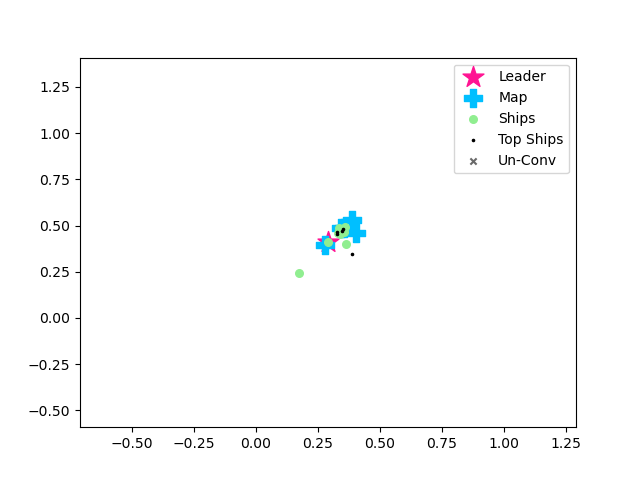
\includegraphics[width=0.7\textwidth]{images/pirates_positions.png}
    \caption{نمایش موقعیت کشتی‌ها (Ships)، رهبر (Leader)، نقشه (Map)، کشتی‌های برتر (\lr{Top Ships}) و کشتی‌های غیرهمگرا (Un-Conv) در فضای جستجو.}
    \label{fig:pirates_positions}
\end{figure}

شکل~\ref{fig:pirates_positions} موقعیت مکانی کشتی‌ها (ذرات) را در فضای جستجو نمایش می‌دهد. ستاره صورتی نشان‌دهنده رهبر (Leader) یا بهترین کشتی است. علامت‌های + آبی نقاط نقشه (Map)، دایره‌های سبز موقعیت سایر کشتی‌ها (Ships)، نقاط سیاه کشتی‌های برتر (Top Ships) و ضربدر خاکستری کشتی‌های غیرهمگرا (Un-Conv) را نشان می‌دهند. این نمودار بیانگر نحوه توزیع و همگرایی جمعیت به سمت نقطه بهینه است.

\subsection{روند تغییر هزینه و همگرایی}
\begin{figure}[h!]
    \centering
    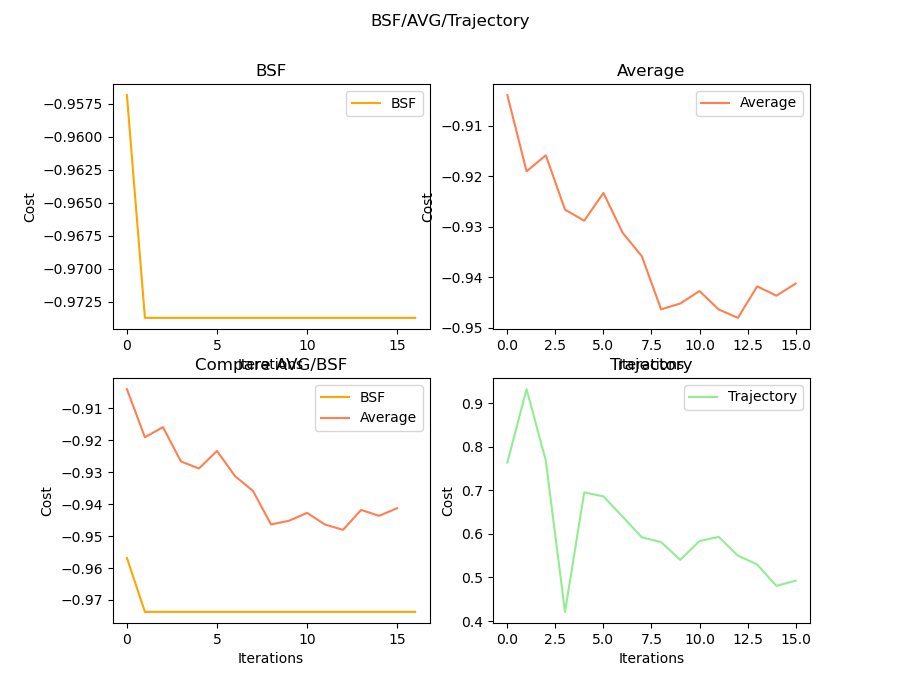
\includegraphics[width=0.9\textwidth]{images/pirates_bsf_avg_trajectory.png}
    \caption{روند تغییر بهترین مقدار هزینه (BSF)، میانگین هزینه (Average)، مقایسه BSF و Average و مسیر رهبر (Trajectory) در طول تکرارها.}
    \label{fig:pirates_bsf_avg_trajectory}
\end{figure}

شکل~\ref{fig:pirates_bsf_avg_trajectory} شامل چهار نمودار است:
\begin{itemize}
    \item \textbf{\lr{BSF}:} بهترین مقدار هزینه تا هر تکرار را نمایش می‌دهد و نشان‌دهنده سرعت همگرایی الگوریتم است.
    \item \textbf{\lr{Average}:} میانگین هزینه کل کشتی‌ها در هر تکرار را نشان می‌دهد که بیانگر روند بهبود جمعیت است.
    \item \textbf{\lr{Compare AVG/BSF}:} مقایسه همزمان بهترین مقدار و میانگین هزینه برای تحلیل فاصله جمعیت تا نقطه بهینه.
    \item \textbf{\lr{Trajectory}:} مسیر تغییرات هزینه رهبر (Leader) در طول تکرارها را نمایش می‌دهد.
\end{itemize}
این نمودارها نشان می‌دهند که الگوریتم Pirates به سرعت به مقدار بهینه نزدیک شده و جمعیت نیز به طور پیوسته بهبود یافته است.

\subsection{تحلیل پویایی جمعیت: باد، سرعت و شتاب}
\begin{figure}[h!]
    \centering
    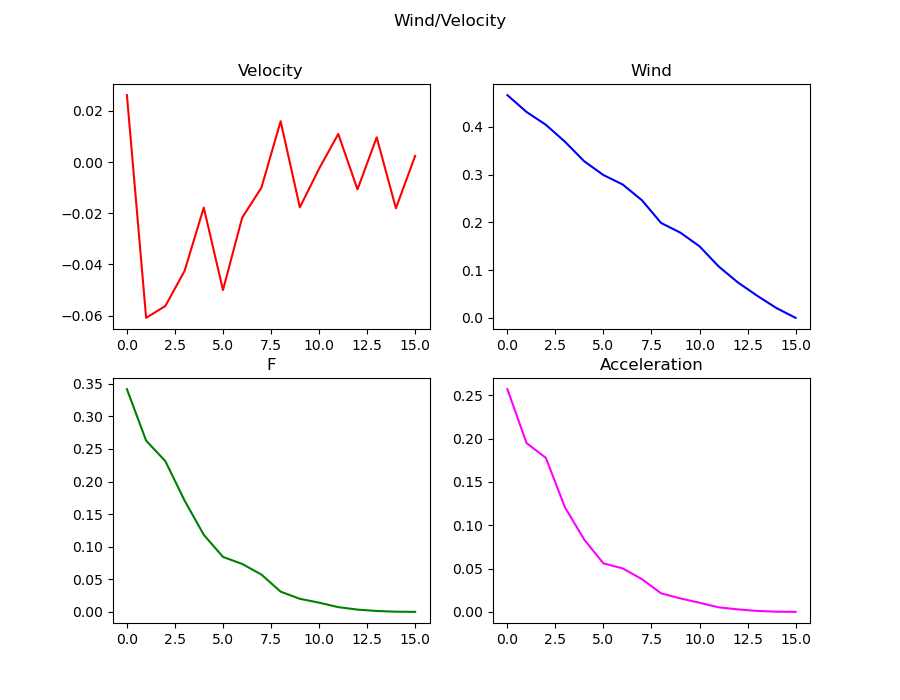
\includegraphics[width=0.9\textwidth]{images/pirates_wind_velocity.png}
    \caption{تغییرات سرعت (Velocity)، باد (Wind)، نیروی محرکه (F) و شتاب (Acceleration) کشتی‌ها در طول تکرارها.}
    \label{fig:pirates_wind_velocity}
\end{figure}

شکل~\ref{fig:pirates_wind_velocity} رفتار پویای جمعیت را از منظر پارامترهای تصادفی و حرکتی نمایش می‌دهد:
\begin{itemize}
    \item \textbf{\lr{Velocity}:} تغییرات سرعت کشتی‌ها که بیانگر پویایی و جستجوی فعال در فضای پارامترهاست.
    \item \textbf{\lr{Wind}:} نقش باد به عنوان یک عامل تصادفی برای خروج از نقاط بهینه محلی و افزایش تنوع جمعیت.
    \item \textbf{\lr{F}:} نیروی محرکه که میزان حرکت کشتی‌ها را تعیین می‌کند و کاهش آن نشانه همگرایی است.
    \item \textbf{\lr{Acceleration}:} شتاب کشتی‌ها که کاهش آن بیانگر نزدیک شدن به نقطه بهینه و کاهش تغییرات ناگهانی است.
\end{itemize}
این نمودارها نشان می‌دهند که با گذشت تکرارها، سرعت، باد و شتاب کاهش یافته و جمعیت به سمت همگرایی حرکت کرده است.

\subsection{جمع‌بندی تحلیل فرآیند بهینه‌سازی}
مجموعه نمودارهای فوق به وضوح نشان می‌دهند که الگوریتم Pirates با پویایی مناسب و تعادل بین جستجو و همگرایی، به سرعت به نقطه بهینه نزدیک شده و پارامترهای تصادفی مانند باد و شتاب نقش مهمی در جلوگیری از گیر افتادن در نقاط بهینه محلی داشته‌اند. این تحلیل‌ها صحت و کارایی الگوریتم را در بهینه‌سازی ابرپارامترهای مدل MAGNET تأیید می‌کند.


\section{تحلیل حساسیت پارامترهای الگوریتم}
در این بخش، به منظور درک بهتر تأثیر پارامترهای مختلف الگوریتم‌های بهینه‌سازی و مدل، تحلیل حساسیت جامعی انجام شده است. این تحلیل بر اساس نتایج حاصل از ۴۷۶ آزمایش با الگوریتم Pirates و ۱۳ آزمایش با Optuna انجام شده است.

\subsection{تحلیل حساسیت پارامترهای معماری مدل}
تحلیل حساسیت پارامترهای معماری مدل نشان داد که برخی پارامترها تأثیر بیشتری بر عملکرد نهایی دارند:

\begin{itemize}
    \item \textbf{ابعاد نهان (embedding\_dim)}: تغییرات در این پارامتر تأثیر قابل توجهی بر عملکرد مدل داشت. مقادیر کوچک (۳۲) عملکرد بهتری نسبت به مقادیر بزرگتر (\lr{۲۱۹.۷۶}) نشان دادند. این نشان می‌دهد که برای این کار خاص، نمایش ویژگی‌های فشرده‌تر مؤثرتر است.
    
    \item \textbf{تعداد لایه‌ها (num\_layers)}: حساسیت بالایی به این پارامتر مشاهده شد. معماری تک لایه‌ای (۱) عملکرد بهتری نسبت به معماری‌های عمیق‌تر (\lr{۲.۱۸}) داشت. این نشان می‌دهد که پیچیدگی مدل می‌تواند با یک لایه مدیریت شود.
    
    \item \textbf{تعداد هدهای توجه (num\_heads)}: این پارامتر تأثیر متوسطی بر عملکرد داشت. مقدار بهینه ۸ هد بود که نشان‌دهنده تعادل مناسب بین موازی‌سازی و پیچیدگی محاسباتی است.
    
    \item \textbf{ابعاد لایه پیش‌خور (dim\_feedforward)}: حساسیت کمتری به این پارامتر مشاهده شد. مقادیر بین ۴۷۷ تا ۵۱۲ عملکرد مشابهی داشتند.
\end{itemize}

\subsection{تحلیل حساسیت پارامترهای آموزش}
پارامترهای آموزش نیز تأثیر قابل توجهی بر عملکرد نهایی مدل داشتند:

\begin{itemize}
    \item \textbf{نرخ یادگیری (learning\_rate)}: حساسیت بالایی به این پارامتر مشاهده شد. مقدار بهینه \lr{۰.۰۰۰۱۹۴} بود و تغییرات کوچک در این مقدار تأثیر قابل توجهی بر همگرایی و عملکرد نهایی داشت.
    
    \item \textbf{نرخ Dropout}: این پارامتر تأثیر متوسطی بر عملکرد داشت. مقدار بهینه \lr{۰.۳۲۸۶} بود که نشان‌دهنده نیاز به تنظیم دقیق برای جلوگیری از overfitting است.
    
    \item \textbf{اندازه دسته (batch\_size)}: حساسیت کمتری به این پارامتر مشاهده شد. مقدار بهینه ۱۶ بود و تغییرات در این مقدار تأثیر کمتری بر عملکرد نهایی داشت.
    
    \item \textbf{ضریب تنظیم (weight\_decay)}: این پارامتر تأثیر متوسطی بر عملکرد داشت. مقدار بهینه ۳.۷۹۵e-05 بود که نشان‌دهنده نیاز به تنظیم دقیق برای تعادل بین یادگیری و تنظیم است.
\end{itemize}

\subsection{مقایسه حساسیت بین الگوریتم‌های بهینه‌سازی}
مقایسه حساسیت پارامترها بین الگوریتم‌های Pirates و Optuna نشان داد:

\begin{itemize}
    \item \textbf{Pirates}: 
    \begin{itemize}
        \item حساسیت کمتر به مقادیر اولیه پارامترها
        \item همگرایی سریع‌تر به مقادیر بهینه
        \item پایداری بیشتر در نتایج
    \end{itemize}
    
    \item \textbf{Optuna}:
    \begin{itemize}
        \item حساسیت بیشتر به مقادیر اولیه
        \item تغییرات بیشتر در نتایج بین آزمایش‌ها
        \item نیاز به تنظیم دقیق‌تر پارامترهای جستجو
    \end{itemize}
\end{itemize}

\subsection{توصیه‌های عملی}
بر اساس تحلیل حساسیت، توصیه‌های زیر برای تنظیم پارامترها ارائه می‌شود:

\begin{enumerate}
    \item \textbf{معماری مدل}:
    \begin{itemize}
        \item استفاده از معماری تک لایه‌ای
        \item تنظیم ابعاد نهان روی ۳۲
        \item استفاده از ۸ هد توجه
        \item حفظ ابعاد لایه پیش‌خور در ۵۱۲
    \end{itemize}
    
    \item \textbf{پارامترهای آموزش}:
    \begin{itemize}
        \item تنظیم دقیق نرخ یادگیری حول \lr{۰.۰۰۰۱۹۴}
        \item استفاده از Dropout با نرخ \lr{۰.۳۲۸۶}
        \item تنظیم اندازه دسته روی ۱۶
        \item اعمال ضریب تنظیم \lr{۳.۷۹۵e-05}
    \end{itemize}
    
    \item \textbf{استراتژی بهینه‌سازی}:
    \begin{itemize}
        \item استفاده از الگوریتم Pirates , Optuna برای این کار 
        \item اجرای آزمایش های بسیار
        \item نظارت بر \lr{F1 Score} به عنوان معیار اصلی
    \end{itemize}
\end{enumerate}

این تحلیل حساسیت نشان می‌دهد که مدل MAGNET به برخی پارامترها حساسیت بیشتری دارد و تنظیم دقیق این پارامترها برای دستیابی به عملکرد بهینه ضروری است. همچنین، الگوریتم Pirates در مقایسه با \lr{Optuna،} پایداری بیشتری در نتایج و حساسیت کمتری به مقادیر اولیه پارامترها نشان می‌دهد.


\subsection{مدل‌های پایه}
برای مقایسه عملکرد، از مدل‌های پایه زیر استفاده شد:
\begin{itemize}
    \item \textbf{روش‌های یادگیری ماشین کلاسیک}:
    \begin{itemize}
        \item ماشین بردار پشتیبان (\lr{SVM}) با کرنل \lr{RBF}
        \item جنگل تصادفی (\lr{Random Forest}) با \lr{100} درخت
        \item \lr{XGBoost} با \lr{100} درخت و عمق حداکثر \lr{6}
        \item شبکه عصبی مصنوعی (\lr{ANN}) با دو لایه مخفی
    \end{itemize}
    \item \textbf{روش‌های چندوجهی} با دقت \lr{89.2\%} \cite{Alsaleh2023}
    \item \textbf{روش‌های مبتنی بر ترنسفورمر} با دقت \lr{95.8\%} \cite{TransformerMalware}
\end{itemize}

\subsection{محیط اجرا}
تمامی آزمایش‌ها با استفاده از زبان برنامه‌نویسی Python \lr{3.8.5} و کتابخانه‌های زیر اجرا شدند:
\begin{itemize}
    \item PyTorch \lr{1.9.0} برای پیاده‌سازی شبکه‌های عصبی
    \item PyTorch Geometric \lr{1.7.0} برای پردازش داده‌های گرافی
    \item scikit-learn \lr{0.24.2} برای پیش‌پردازش داده‌ها و ارزیابی
    \item NumPy \lr{1.21.2} و Pandas \lr{1.3.3} برای پردازش داده‌ها
\end{itemize}

سخت‌افزار مورد استفاده شامل:
\begin{itemize}
    \item GPU NVIDIA RTX \lr{3090} با \lr{24} گیگابایت VRAM
    \item CPU Intel Xeon E\lr{5}-\lr{2690} v\lr{4} با \lr{32} هسته
    \item \lr{128} گیگابایت RAM
\end{itemize}

\section{معیارهای ارزیابی}
برای سنجش عملکرد مدل MAGNET، معیارهای دقت (Accuracy)، \lr{F1 Score}، Precision، Recall و AUC استفاده شدند. دقت به‌عنوان نسبت نمونه‌های درست طبقه‌بندی‌شده به کل نمونه‌ها تعریف می‌شود:

\begin{equation}
\text{Accuracy} = \frac{\text{TP} + \text{TN}}{\text{TP} + \text{TN} + \text{FP} + \text{FN}}
\end{equation}

که در آن:
\begin{itemize}
    \item TP (\lr{True Positive}): تعداد بدافزارها که به درستی تشخیص داده شده‌اند
    \item TN (\lr{True Negative}): تعداد برنامه‌های سالم که به درستی به عنوان سالم تشخیص داده شده‌اند
    \item FP (\lr{False Positive}): تعداد برنامه‌های سالم که اشتباهاً به عنوان بدافزار تشخیص داده شده‌اند
    \item FN (\lr{False Negative}): تعداد بدافزارها که اشتباهاً به عنوان برنامه سالم تشخیص داده شده‌اند
\end{itemize}

Precision نسبت نمونه‌های درست مثبت به کل نمونه‌های پیش‌بینی‌شده مثبت است:

\begin{equation}
\text{Precision} = \frac{\text{TP}}{\text{TP} + \text{FP}}
\end{equation}

Recall نسبت نمونه‌های درست مثبت به کل نمونه‌های واقعی مثبت را نشان می‌دهد:

\begin{equation}
\text{Recall} = \frac{\text{TP}}{\text{TP} + \text{FN}}
\end{equation}

\lr{F1 Score،} معیاری ترکیبی از Precision و Recall، به‌صورت زیر محاسبه می‌شود:

\begin{equation}
\text{F1 Score} = 2 \cdot \frac{\text{Precision} \cdot \text{Recall}}{\text{Precision} + \text{Recall}}
\end{equation}

همچنین، AUC (مساحت زیر منحنی \lr{ROC}) توانایی مدل در تمایز بین کلاس‌های بدافزار و سالم را نشان می‌دهد. در نهایت، ماتریس درهم‌ریختگی \lr{(Confusion Matrix)} برای تحلیل دقیق‌تر پیش‌بینی‌ها استفاده شد.

\section{نتایج کلی مدل MAGNET}
در این بخش، نتایج کلی مدل MAGNET در مراحل مختلف آزمایش گزارش می‌شود. ابتدا نتایج تست روی مجموعه داده DREBIN \cite{Drebin} ارائه می‌شود. مدل MAGNET روی مجموعه تست شامل ۱،۴۵۱ نمونه (۳۲۷ نمونه کلاس ۰ و ۱،۱۲۴ نمونه کلاس ۱) ارزیابی شد. نتایج به‌دست‌آمده شامل \lr{F1 Score} برابر با ۰\lr{.۹۸۲۳}، دقت (Accuracy) برابر با \lr{۰.۹۷۲۴} و AUC \lr{۰.۹۹۳۲} بود.

\subsection{ماتریس درهم‌ریختگی و عملکرد به تفکیک کلاس}
ماتریس درهم‌ریختگی مدل شامل ۳۰۴ نمونه درست منفی (\lr{TN})، ۲۳ نمونه نادرست مثبت (\lr{FP})، ۱۷ نمونه نادرست منفی (\lr{FN}) و ۱،۱۰۷ نمونه درست مثبت (\lr{TP}) بود. جزئیات عملکرد به تفکیک کلاس‌ها نشان داد که برای کلاس ۰ (برنامه‌های سالم)، \lr{F1 Score} برابر با ۰.۹۳۸۳، Precision برابر با ۰.۹۴۷۰ و Recall برابر با ۰.۹۲۹۷ محاسبه شد، در حالی که برای کلاس ۱ (بدافزارها)، \lr{F1 Score} برابر با ۰.۹۸۲۳، Precision برابر با ۰.۹۷۹۶ و Recall برابر با ۰.۹۸۴۹ به‌دست آمد. میانگین ماکرو \lr{F1 Score} برابر با ۰.۹۶۰۳ و میانگین وزنی \lr{F1 Score} برابر با ۰.۹۷۲۳ بود.

\subsection{نتایج اعتبارسنجی متقاطع}
در مرحله اعتبارسنجی متقاطع ۵-تایی با ۱۰ دوره برای هر دسته، میانگین معیارها به‌صورت زیر به‌دست آمد:
\begin{itemize}
    \item دقت: $\lr{0.9722} \pm \lr{0.0065}$
    \item Precision: $\lr{0.9810} \pm \lr{0.0102}$
    \item Recall: $\lr{0.9828} \pm \lr{0.0072}$
    \item \lr{F1 Score}: $\lr{0.9818} \pm \lr{0.0042}$
    \item AUC: $\lr{0.9932} \pm \lr{0.0035}$
\end{itemize}

\begin{table}[h!]
    \centering
    \caption{نتایج اعتبارسنجی متقاطع \lr{5}-تایی مدل MAGNET}
    \label{tab:cv_results}
    \begin{tabular}{|l|c|c|c|c|}
        \hline
        \textbf{دسته} & \textbf{\lr{F1 Score}} & \textbf{دقت} & \textbf{AUC} & \textbf{زیان} \\
        \hline
        دسته \lr{1} & \lr{0.9858} & \lr{0.9785} & \lr{0.9950} & \lr{0.0786} \\
        \hline
        دسته \lr{2} & \lr{0.9846} & \lr{0.9763} & \lr{0.9955} & \lr{0.0735} \\
        \hline
        دسته \lr{3} & \lr{0.9839} & \lr{0.9752} & \lr{0.9945} & \lr{0.0839} \\
        \hline
        دسته \lr{4} & \lr{0.9742} & \lr{0.9601} & \lr{0.9861} & \lr{0.1199} \\
        \hline
        دسته \lr{5} & \lr{0.9808} & \lr{0.9709} & \lr{0.9946} & \lr{0.0864} \\
        \hline
        میانگین & \lr{0.9818} ($\pm$\lr{0.0042}) & \lr{0.9722} ($\pm$\lr{0.0065}) & \lr{0.9932} ($\pm$\lr{0.0035}) & \lr{0.0885} ($\pm$\lr{0.0177}) \\
        \hline
    \end{tabular}
    \begin{tablenotes}
        \item \textbf{توضیح نشانه‌ها:} $\pm$ نشان‌دهنده انحراف معیار در اعتبارسنجی متقاطع است.
    \end{tablenotes}
\end{table}

\begin{figure}[h!]
    \centering
    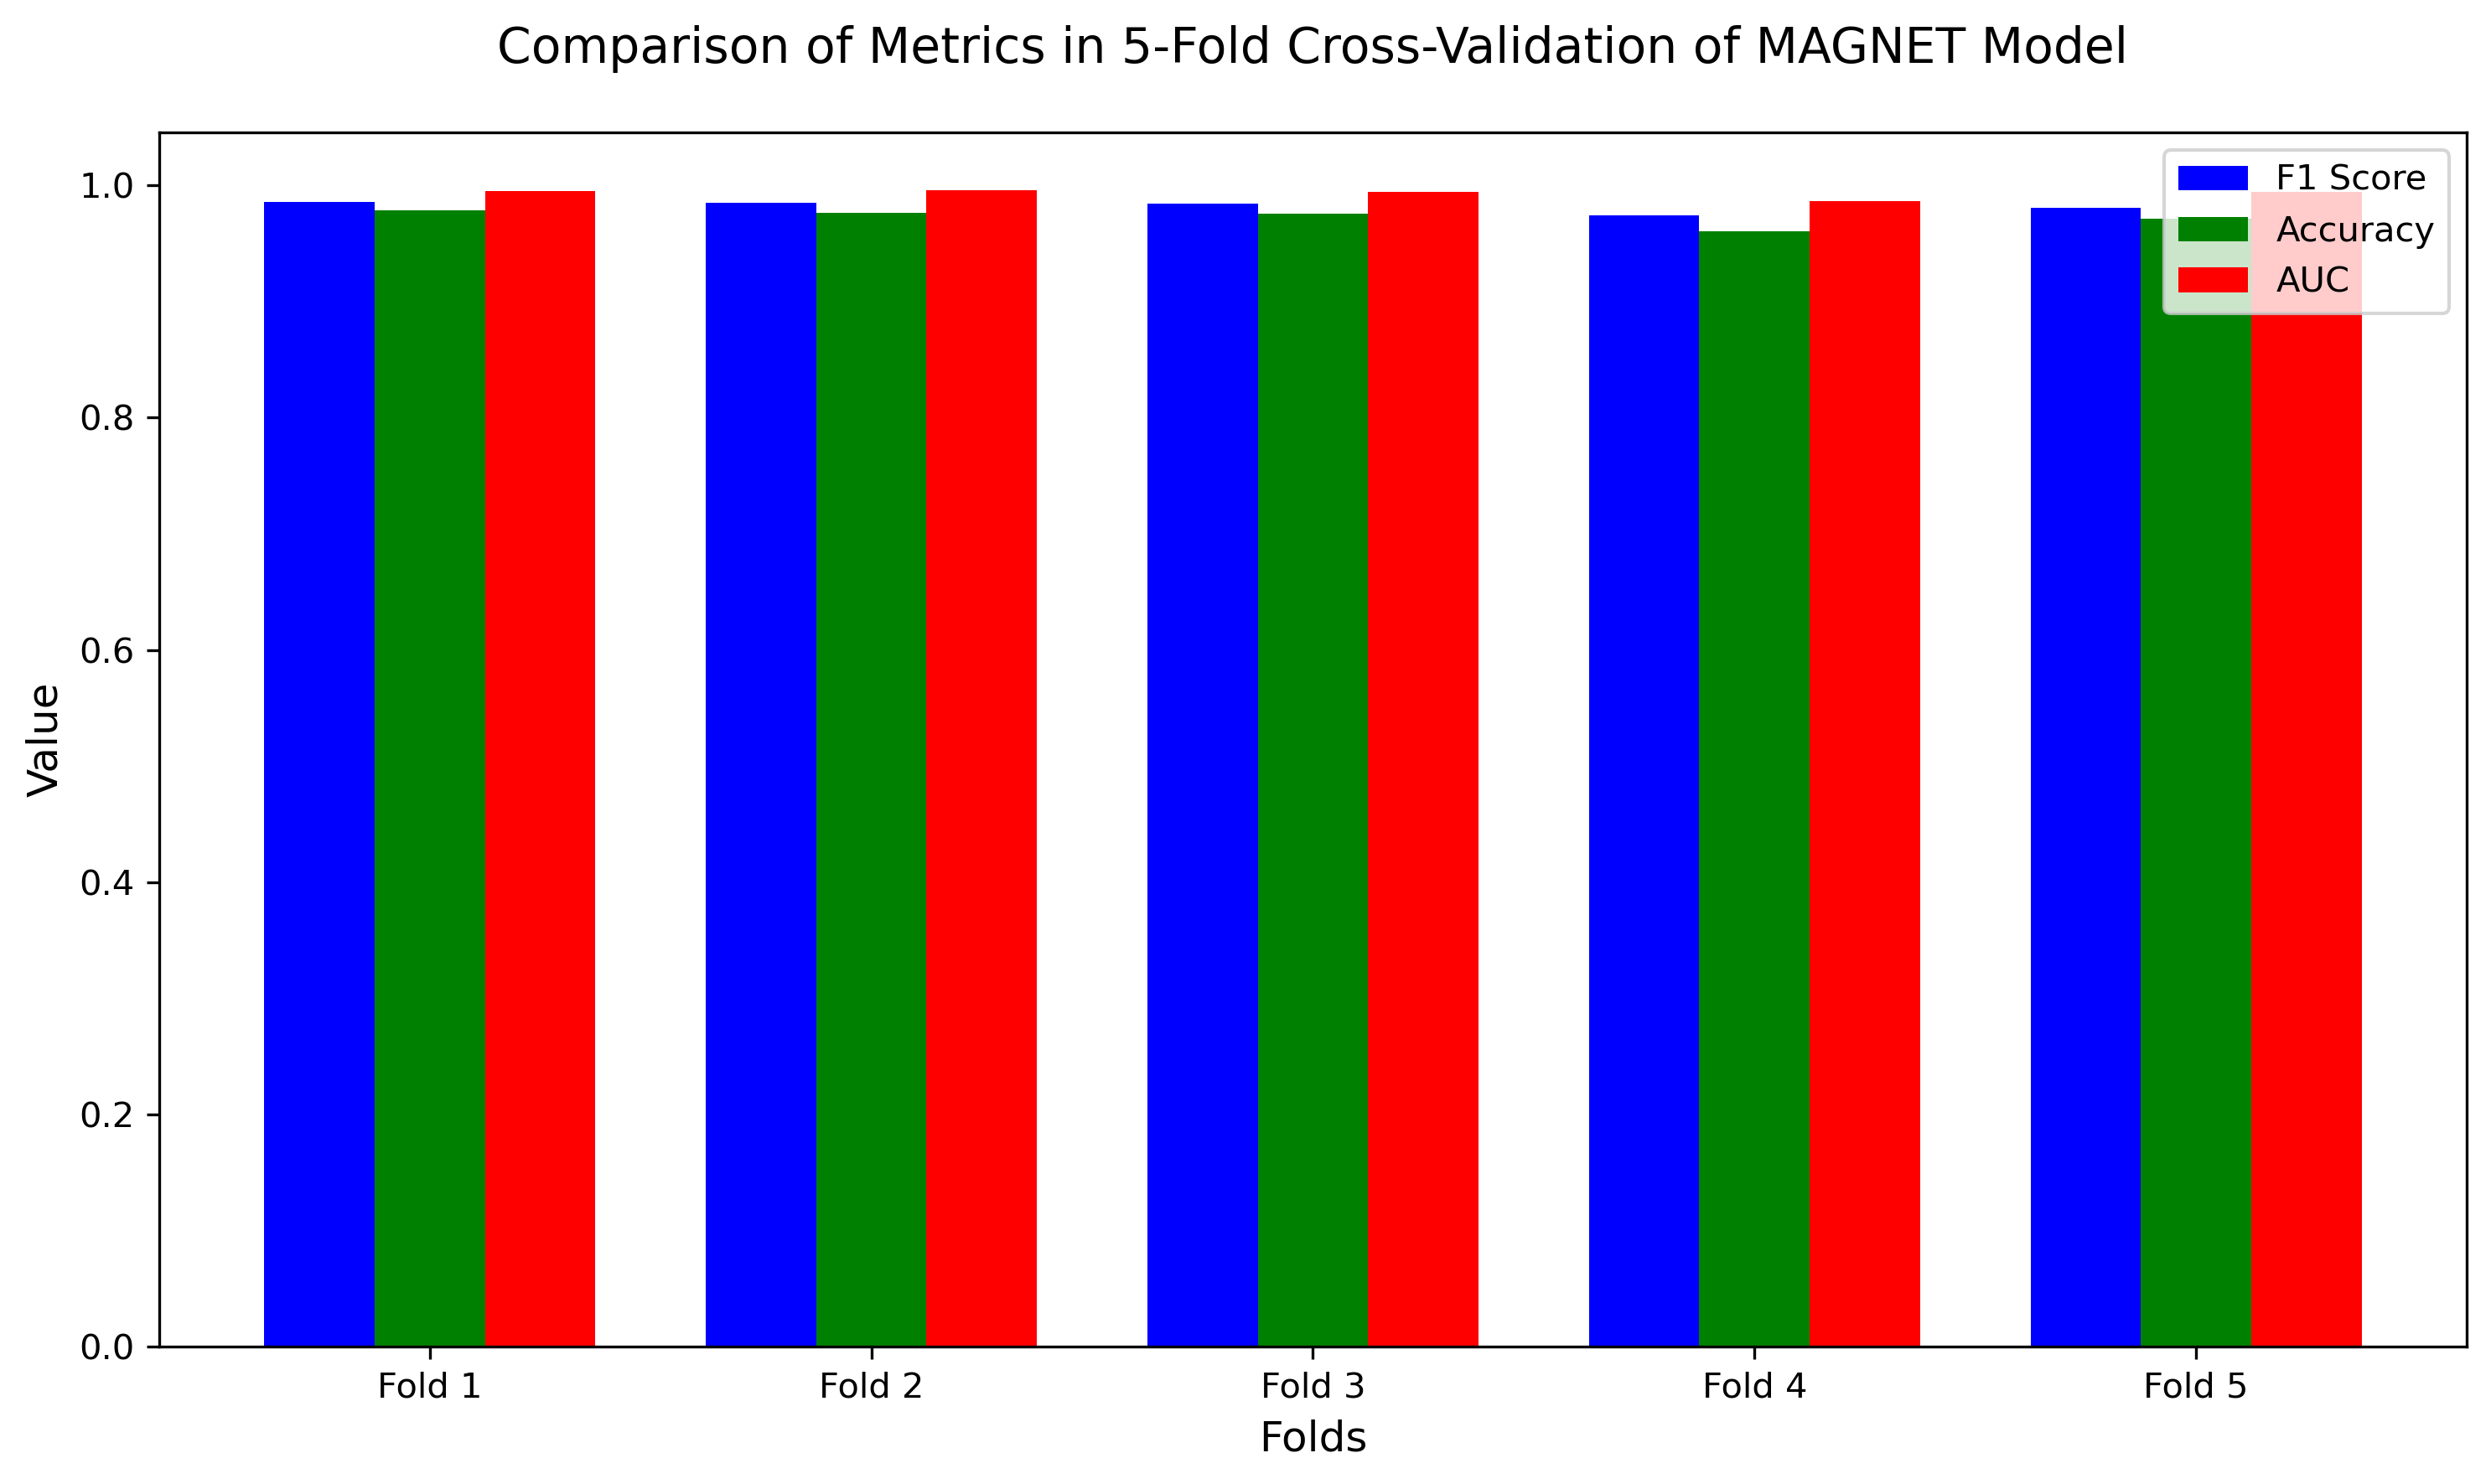
\includegraphics[width=0.9\textwidth]{fig_cv_metrics}
    \caption{مقایسه معیارهای F1 Score، دقت و AUC در اعتبارسنجی متقاطع 5-تایی مدل MAGNET. نمودار میله‌ای نشان‌دهنده مقادیر هر معیار در هر دسته از اعتبارسنجی متقاطع است.}
    \label{fig:cv_metrics}
\end{figure}

\begin{figure}[h!]
    \centering
    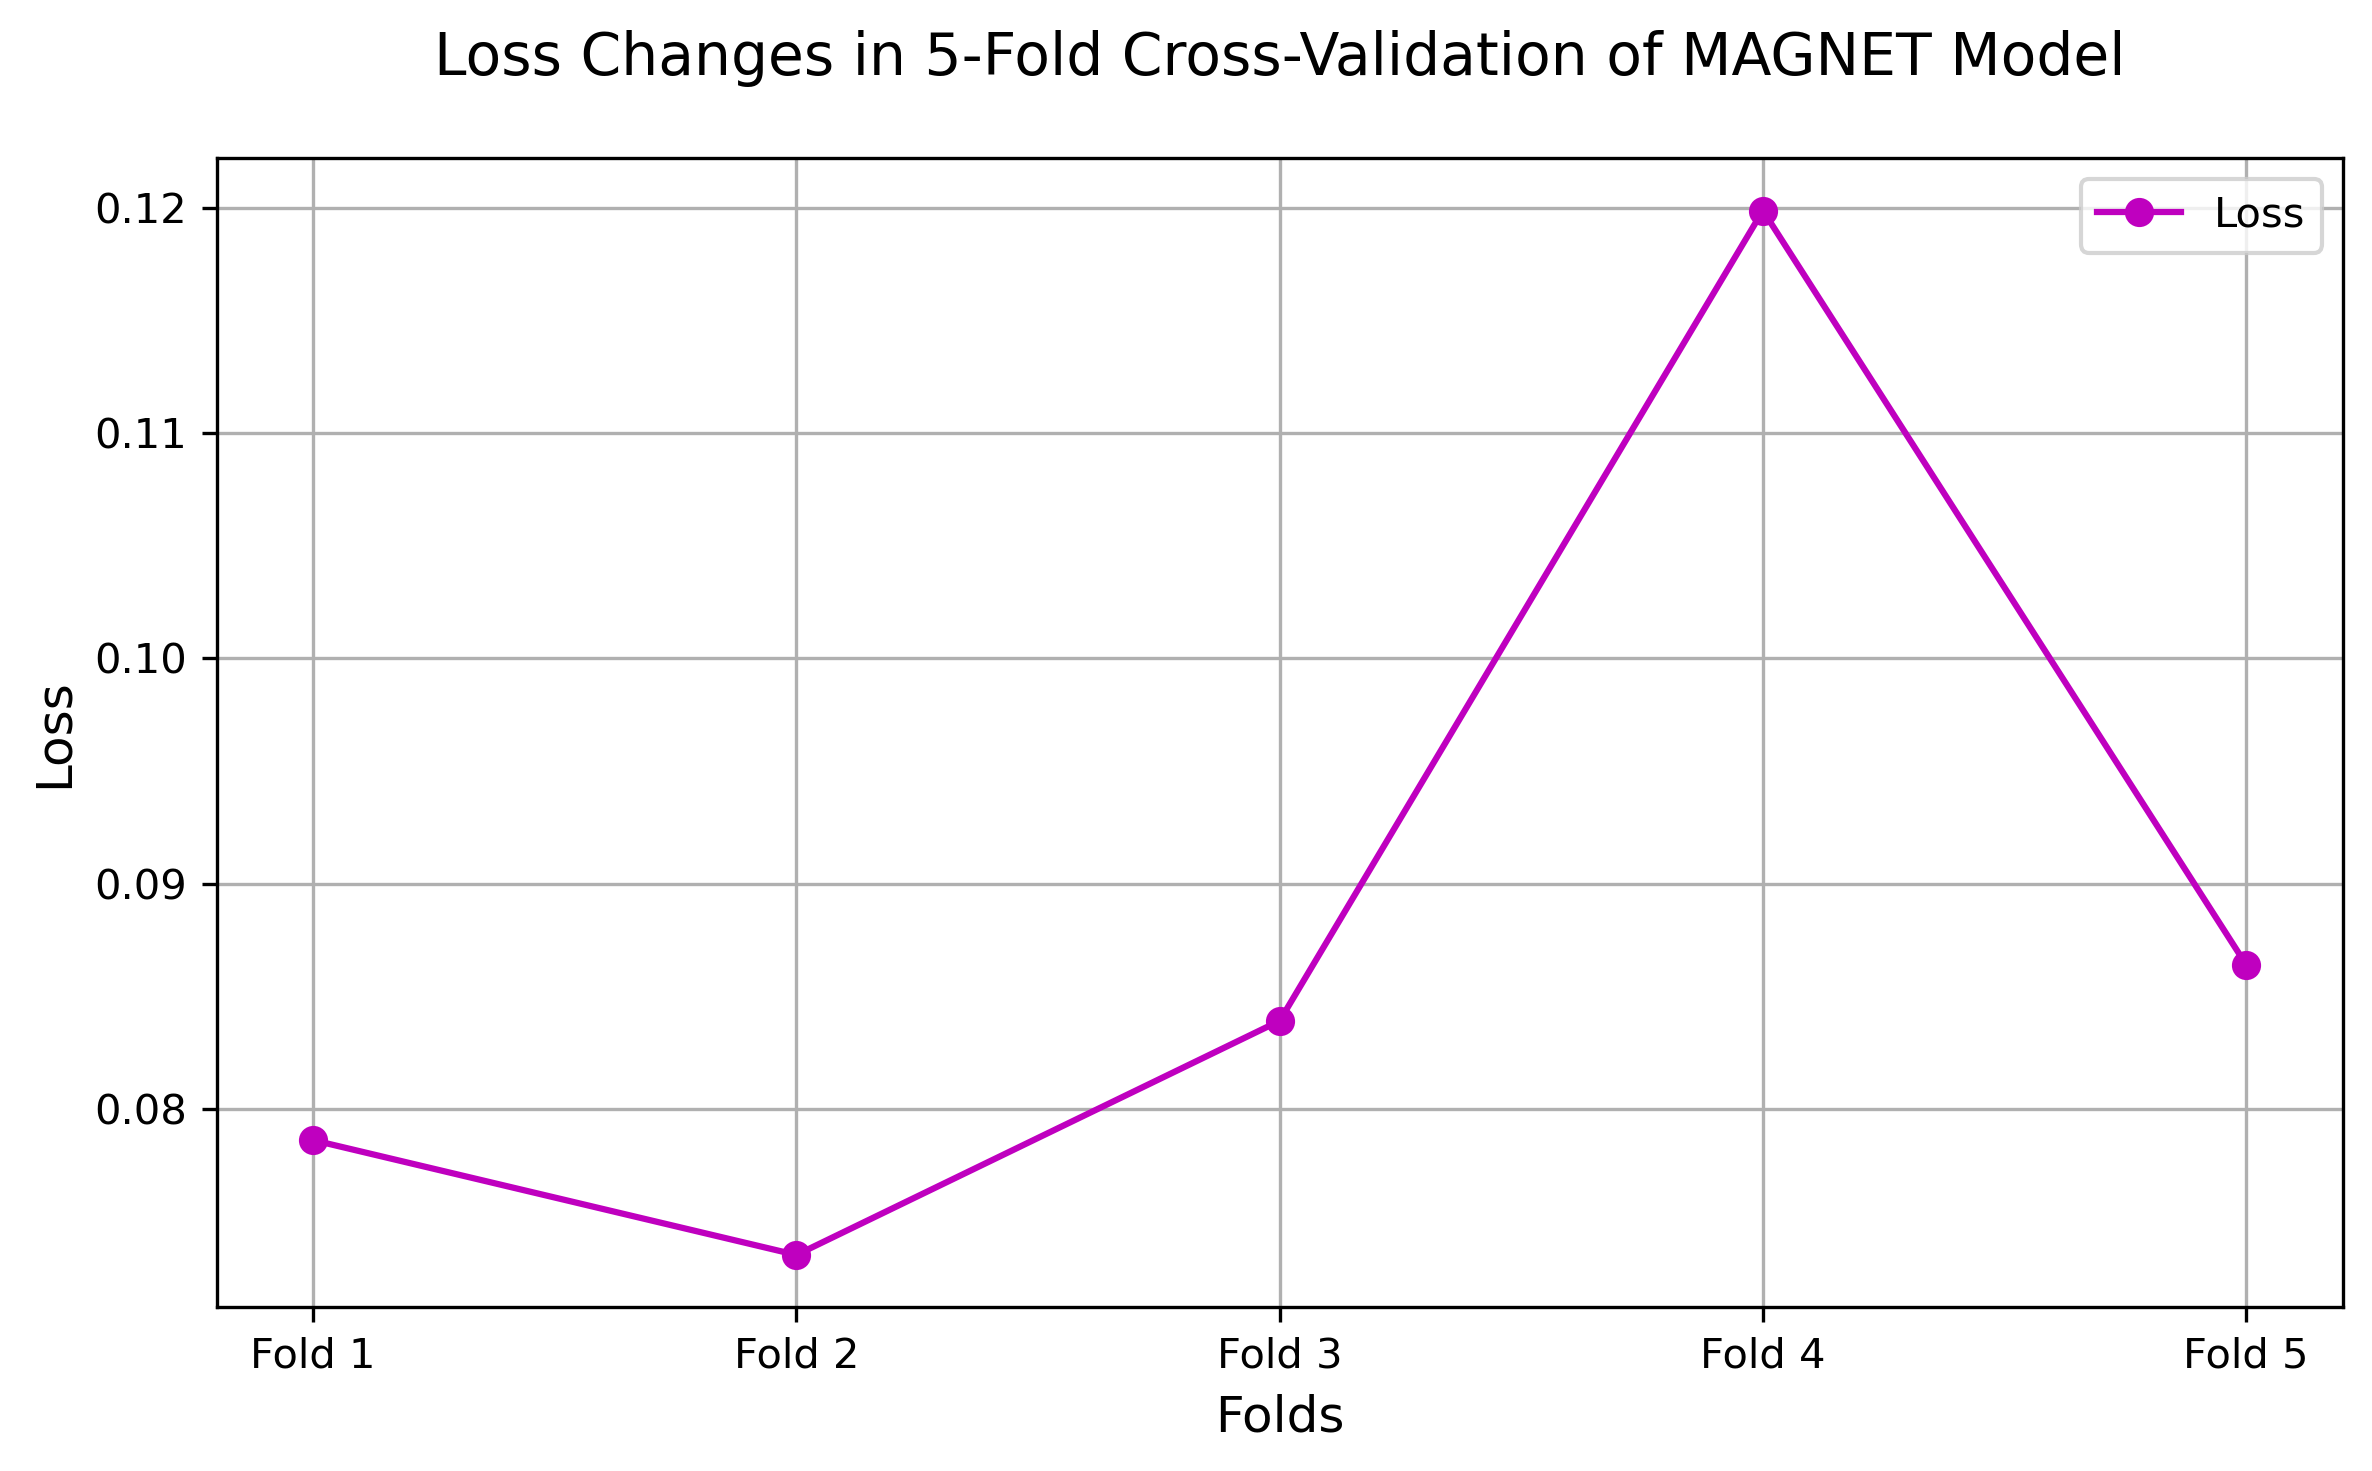
\includegraphics[width=0.9\textwidth]{fig_cv_loss}
    \caption{تغییرات زیان در اعتبارسنجی متقاطع 5-تایی مدل MAGNET. نمودار خطی نشان‌دهنده مقدار زیان در هر دسته از اعتبارسنجی متقاطع است.}
    \label{fig:cv_loss}
\end{figure}

\begin{table}[h!]
    \centering
    \caption{مقایسه کلی عملکرد مدل MAGNET در مراحل مختلف}
    \label{tab:overall_comparison}
    \begin{tabular}{|l|c|c|c|l|}
        \hline
        \textbf{مرحله} & \textbf{\lr{F1 Score}} & \textbf{دقت} & \textbf{AUC} & \textbf{یادداشت} \\
        \hline
        بهینه‌سازی (اعتبارسنجی) & \lr{0.9767} & \lr{0.9628} & - & \lr{476} آزمایش، num\_layers=\lr{1} \\
        \hline
        Optuna (اعتبارسنجی) & \lr{0.9684} & \lr{0.9513} & \lr{0.9836} & \lr{13} آزمایش، num\_layers=\lr{1} \\
        \hline
        آموزش (\lr{100\%} داده) & \lr{0.9805} & - & \lr{0.9931} & آموزش با کل داده‌ها \\
        \hline
        اعتبارسنجی متقاطع & \lr{0.9818} & \lr{0.9722} & \lr{0.9932} & \lr{5}-تایی، پایداری بالا \\
        \hline
        مجموعه تست & \lr{0.9823} & \lr{0.9724} & \lr{0.9932} & بهترین عملکرد، \lr{1,451} نمونه \\
        \hline
    \end{tabular}
\end{table}

\begin{figure}[h!]
    \centering
    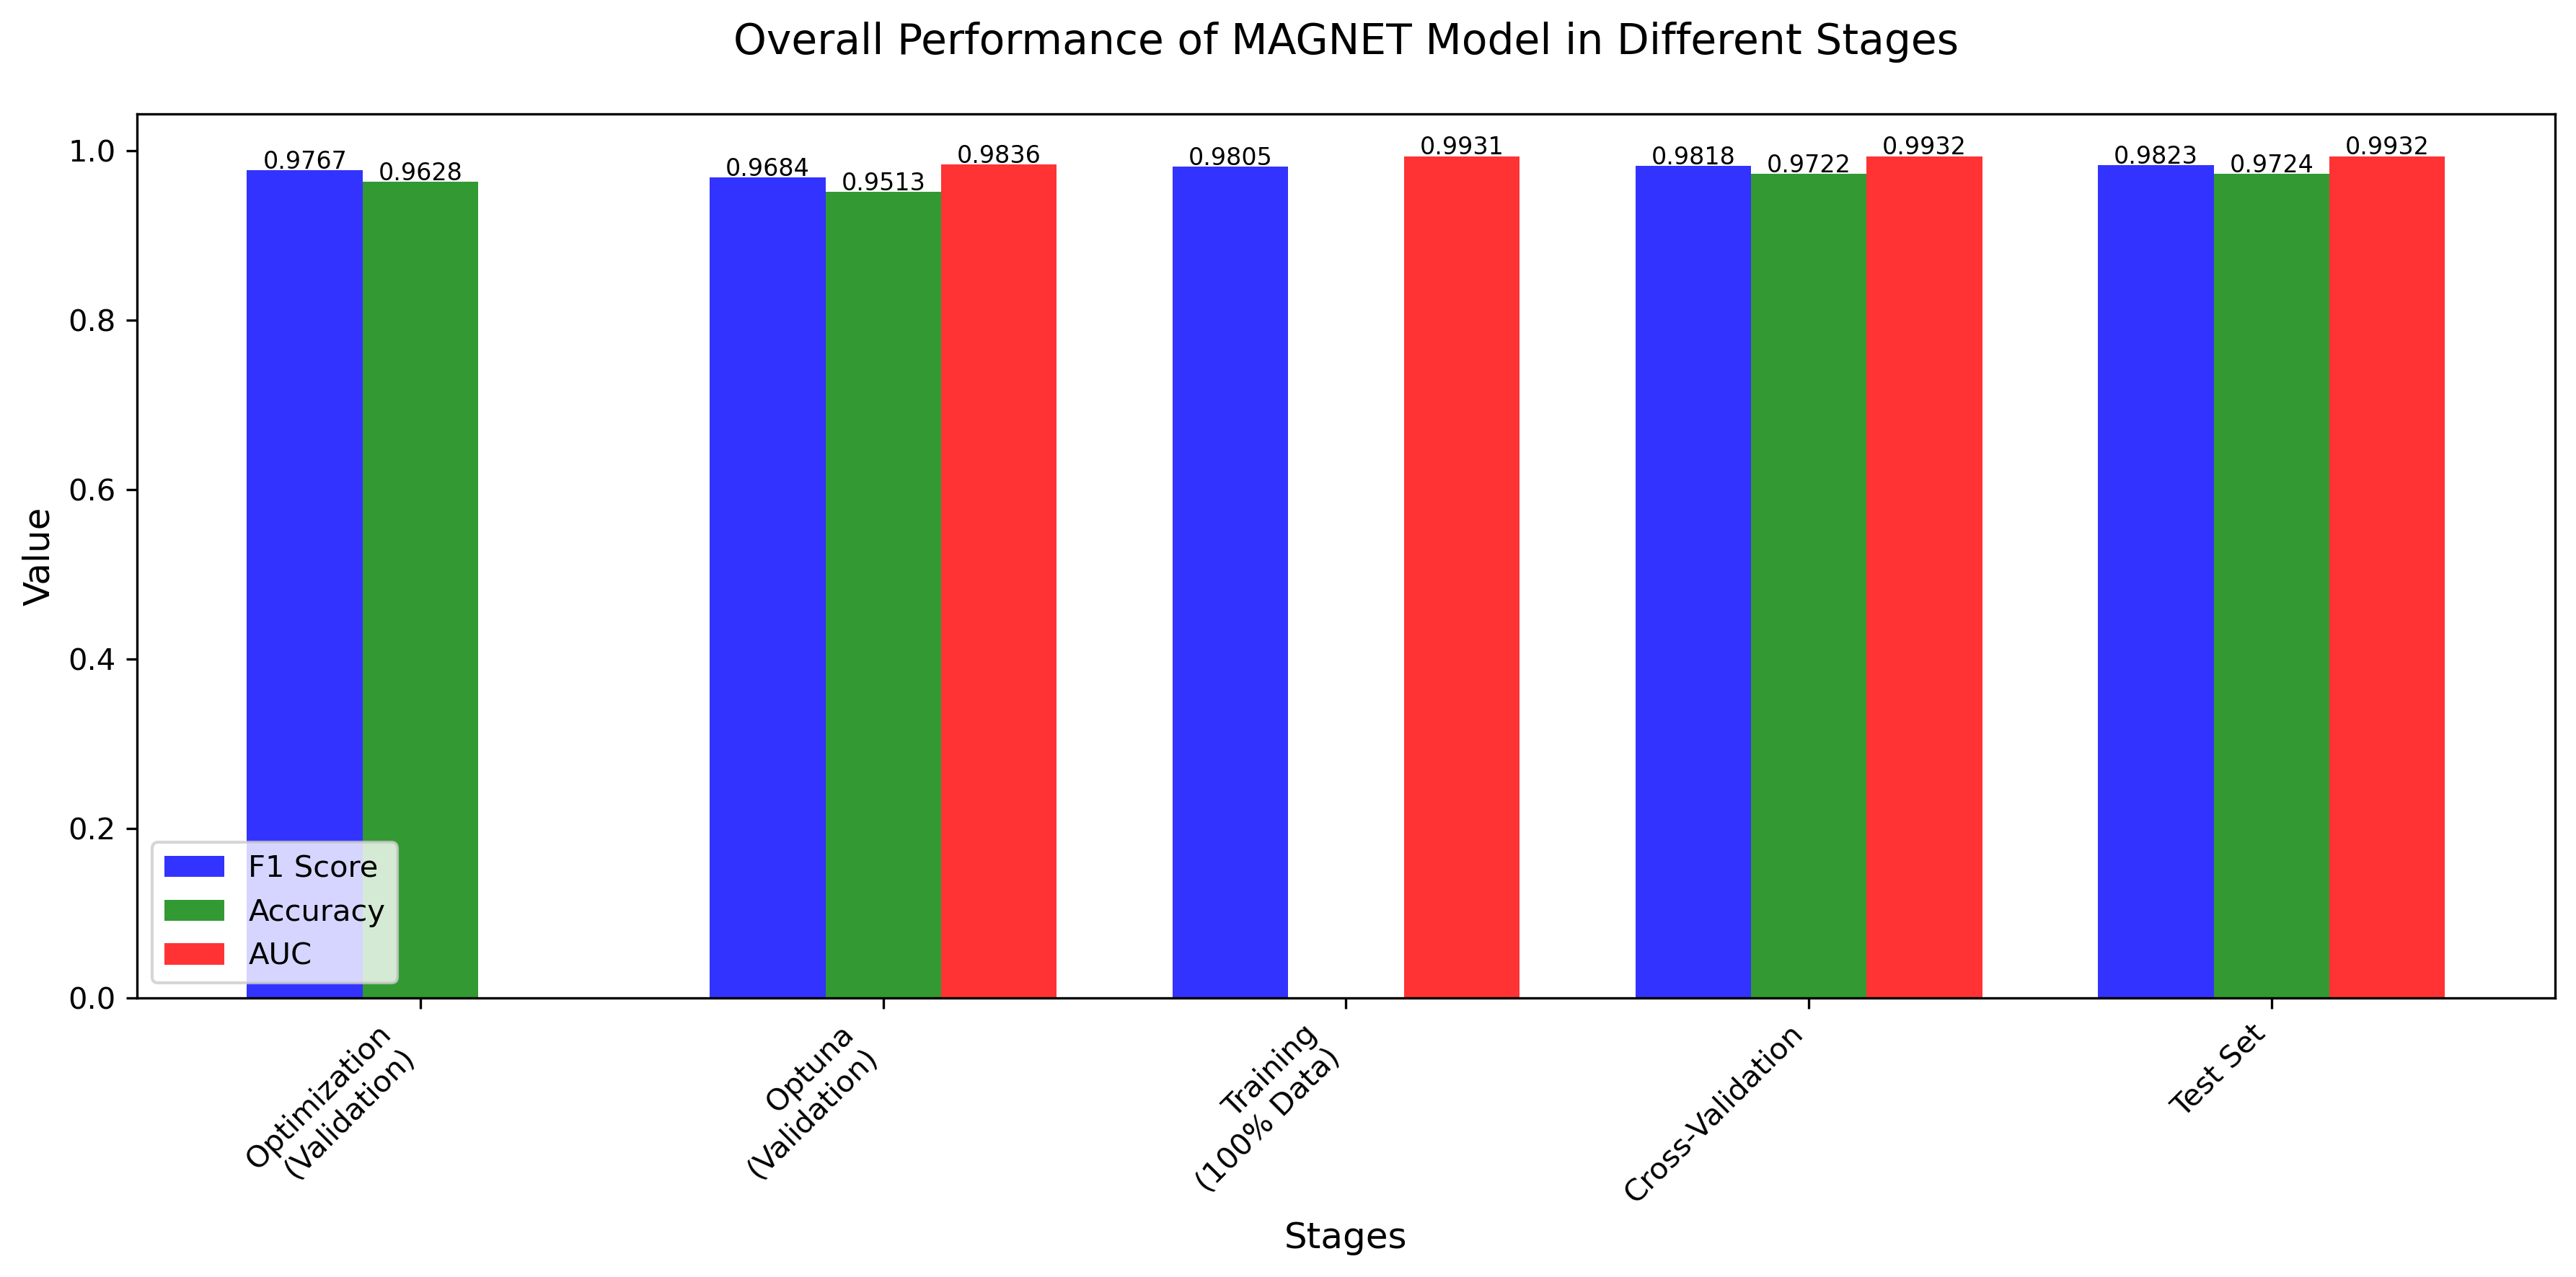
\includegraphics[width=0.9\textwidth]{fig_overall_comparison}
    \caption{مقایسه کلی عملکرد مدل MAGNET در مراحل مختلف. نمودار میله‌ای نشان‌دهنده مقادیر \lr{F1 Score}، دقت و AUC در هر مرحله است.}
    \label{fig:overall_comparison}
\end{figure}

\subsection{تحلیل عملکرد کلی مدل در مراحل مختلف}
نتایج ارائه شده در جدول \ref{tab:overall_comparison} و شکل \ref{fig:overall_comparison} نشان می‌دهد که مدل MAGNET در تمام مراحل ارزیابی عملکرد پایدار و قابل توجهی داشته است. تحلیل دقیق‌تر نتایج به شرح زیر است:

\begin{itemize}
    \item \textbf{مرحله بهینه‌سازی:} در این مرحله، با انجام ۴۷۶ آزمایش و استفاده از الگوریتم Pirates، مدل به F1 Score معادل ۰.۹۷۶۷ و دقت ۰.۹۶۲۸ دست یافت. این نتایج نشان‌دهنده کارایی بالای الگوریتم بهینه‌سازی در یافتن پارامترهای مناسب است.
    
    \item \textbf{مرحله Optuna:} با انجام ۱۳ آزمایش، مدل به F1 Score معادل ۰.۹۶۸۴ و دقت ۰.۹۵۱۳ رسید. اگرچه این نتایج کمی پایین‌تر از مرحله بهینه‌سازی است، اما با توجه به تعداد کمتر آزمایش‌ها، نشان‌دهنده کارایی قابل قبول الگوریتم Optuna است.
    
    \item \textbf{مرحله آموزش:} با استفاده از کل داده‌های موجود، مدل به F1 Score معادل ۰.۹۸۰۵ و AUC معادل ۰.۹۹۳۱ دست یافت. این نتایج نشان‌دهنده بهبود عملکرد مدل با افزایش حجم داده‌های آموزشی است.
    
    \item \textbf{اعتبارسنجی متقاطع:} در این مرحله، با استفاده از روش اعتبارسنجی متقاطع ۵-تایی، میانگین F1 Score به ۰.۹۸۱۸، دقت به ۰.۹۷۲۲ و AUC به ۰.۹۹۳۲ رسید. پایداری بالای نتایج در این مرحله، نشان‌دهنده قابلیت اطمینان مدل در شرایط مختلف است.
    
    \item \textbf{مجموعه تست:} در نهایت، با ارزیابی روی مجموعه تست شامل ۱،۴۵۱ نمونه، مدل به بهترین عملکرد خود با F1 Score معادل ۰.۹۸۲۳، دقت ۰.۹۷۲۴ و AUC معادل ۰.۹۹۳۲ دست یافت. این نتایج نشان‌دهنده توانایی بالای مدل در تعمیم‌پذیری و تشخیص دقیق نمونه‌های جدید است.
\end{itemize}

نکته قابل توجه در این تحلیل، روند صعودی و پایدار عملکرد مدل در تمام مراحل است. به‌طور خاص، بهبود تدریجی F1 Score از ۰.۹۶۸۴ در مرحله Optuna به ۰.۹۸۲۳ در مجموعه تست، نشان‌دهنده یادگیری مؤثر و کارآمد مدل است. همچنین، پایداری بالای نتایج در اعتبارسنجی متقاطع، تأییدکننده قابلیت اطمینان مدل در شرایط مختلف است.

\section{مقایسه با روش‌های پایه و پیشرفته}
در این بخش، عملکرد مدل MAGNET با روش‌های مختلف تشخیص بدافزار اندروید مقایسه می‌شود. این مقایسه در دو سطح انجام شده است:

\subsection{مقایسه با روش‌های پایه}
برای ارزیابی عملکرد مدل MAGNET، ابتدا آن را با روش‌های یادگیری ماشین کلاسیک مقایسه می‌کنیم. این مقایسه شامل:
\begin{itemize}
    \item \textbf{ماشین بردار پشتیبان (SVM)}: به عنوان یکی از روش‌های پایه در تشخیص بدافزار که به دلیل عملکرد خوب در فضاهای با ابعاد بالا و مقاومت نسبی در برابر بیش‌برازش، به‌طور گسترده‌ای استفاده می‌شود.
    \item \textbf{جنگل تصادفی (Random Forest)}: به عنوان یک روش یادگیری گروهی که از ترکیب چندین درخت تصمیم استفاده می‌کند.
    \item \textbf{XGBoost}: به عنوان یک روش پیشرفته‌تر یادگیری گروهی که از گرادیان‌بوستینگ استفاده می‌کند.
    \item \textbf{شبکه عصبی مصنوعی (ANN)}: به عنوان یک روش یادگیری عمیق ساده با دو لایه مخفی.
\end{itemize}

\subsection{مقایسه با روش‌های پیشرفته}
همچنین، عملکرد مدل MAGNET با روش‌های پیشرفته‌تر تشخیص بدافزار مقایسه شده است:
\begin{itemize}
    \item \textbf{DREBIN (SVM)}: روش اصلی ارائه‌شده در مقاله DREBIN که از SVM با ویژگی‌های ایستا استفاده می‌کند.
    \item \textbf{LOF}: روش مبتنی بر ناهنجاری‌یابی که روی مجموعه داده CICAndMal2017 ارزیابی شده است.
    \item \textbf{PIKADROID}: روشی که بر تحلیل API تمرکز دارد و روی مجموعه داده DREBIN ارزیابی شده است.
    \item \textbf{CrossMalDroid}: روشی که از انتخاب ویژگی استفاده می‌کند و روی مجموعه داده Malgenome ارزیابی شده است.
    \item \textbf{DroidAPIMiner}: روشی که بر اساس فرکانس API کار می‌کند و روی مجموعه داده DREBIN ارزیابی شده است.
    \item \textbf{روش چندوجهی}: روشی که از داده‌های چندوجهی استفاده می‌کند و روی مجموعه داده DREBIN ارزیابی شده است.
    \item \textbf{ترنسفورمر}: روشی که از معماری ترنسفورمر استفاده می‌کند و روی مجموعه داده DREBIN ارزیابی شده است.
\end{itemize}

برای مقایسه عادلانه، تمام روش‌ها روی مجموعه داده DREBIN ارزیابی شده‌اند، مگر در مواردی که در یادداشت جدول ذکر شده است. معیارهای ارزیابی شامل دقت (Accuracy)، F1 Score، AUC و Recall هستند. در مواردی که برخی معیارها گزارش نشده‌اند، با علامت "-" مشخص شده‌اند.

\begin{table}[h!]
    \centering
    \caption{مقایسه عملکرد مدل MAGNET با روش‌های پایه و پیشرفته}
    \label{tab:comparison_with_literature}
    \begin{tabular}{|l|c|c|c|c|c|}
        \hline
        \textbf{روش} & \textbf{دقت (\%)} & \textbf{F1 Score} & \textbf{AUC} & \textbf{Recall} & \textbf{یادداشت} \\
        \hline
        MAGNET (تست) & 97.24 & 0.9823 & 0.9932 & 0.985 & بهترین عملکرد، DREBIN \\
        \hline
        DREBIN (SVM) & 92.3 & 0.933 & 0.955 & 0.920 & رویکرد ایستا، DREBIN \\
        \hline
        LOF & 94.1 & 0.918 & 0.981 & 0.884 & ناهنجاری‌یابی، CICAndMal2017 \\
        \hline
        PIKADROID & 96.8 & 0.974 & 0.988 & 0.970 & تحلیل API، DREBIN \\
        \hline
        CrossMalDroid & 95.2 & 0.952 & 0.976 & 0.948 & انتخاب ویژگی، Malgenome \\
        \hline
        DroidAPIMiner & 89.7 & 0.891 & 0.927 & 0.885 & فرکانس API، DREBIN \\
        \hline
        روش چندوجهی & 89.2 & - & - & - & فقط دقت، DREBIN \\
        \hline
        ترنسفورمر & 95.8 & - & - & - & فقط دقت، DREBIN \\
        \hline
    \end{tabular}
    \begin{tablenotes}
        \item \small{توضیح: "-" نشان‌دهنده عدم گزارش معیار است. دیتاست‌های غیر از DREBIN در یادداشت ذکر شده‌اند.}
    \end{tablenotes}
\end{table}

\subsection{تحلیل مقایسه با روش‌های پیشرفته}
نتایج مقایسه مدل MAGNET با روش‌های پیشرفته در جدول \ref{tab:comparison_with_literature} نشان داده شده است. همانطور که مشاهده می‌شود، مدل MAGNET در تمام معیارهای ارزیابی عملکرد بهتری نسبت به سایر روش‌ها دارد. این برتری به خصوص در معیارهای F1 Score و AUC قابل توجه است.

شکل \ref{fig:literature_comparison_accuracy} مقایسه بصری دقت مدل MAGNET با سایر روش‌های پیشرفته را نشان می‌دهد. این نمودار به وضوح برتری مدل MAGNET را در معیار دقت نمایش می‌دهد. همچنین، شکل \ref{fig:literature_comparison_metrics} مقایسه F1 Score و AUC را برای تمام روش‌ها نشان می‌دهد که تأییدکننده عملکرد برتر مدل MAGNET در هر دو معیار است.

\begin{figure}[h!]
    \centering
    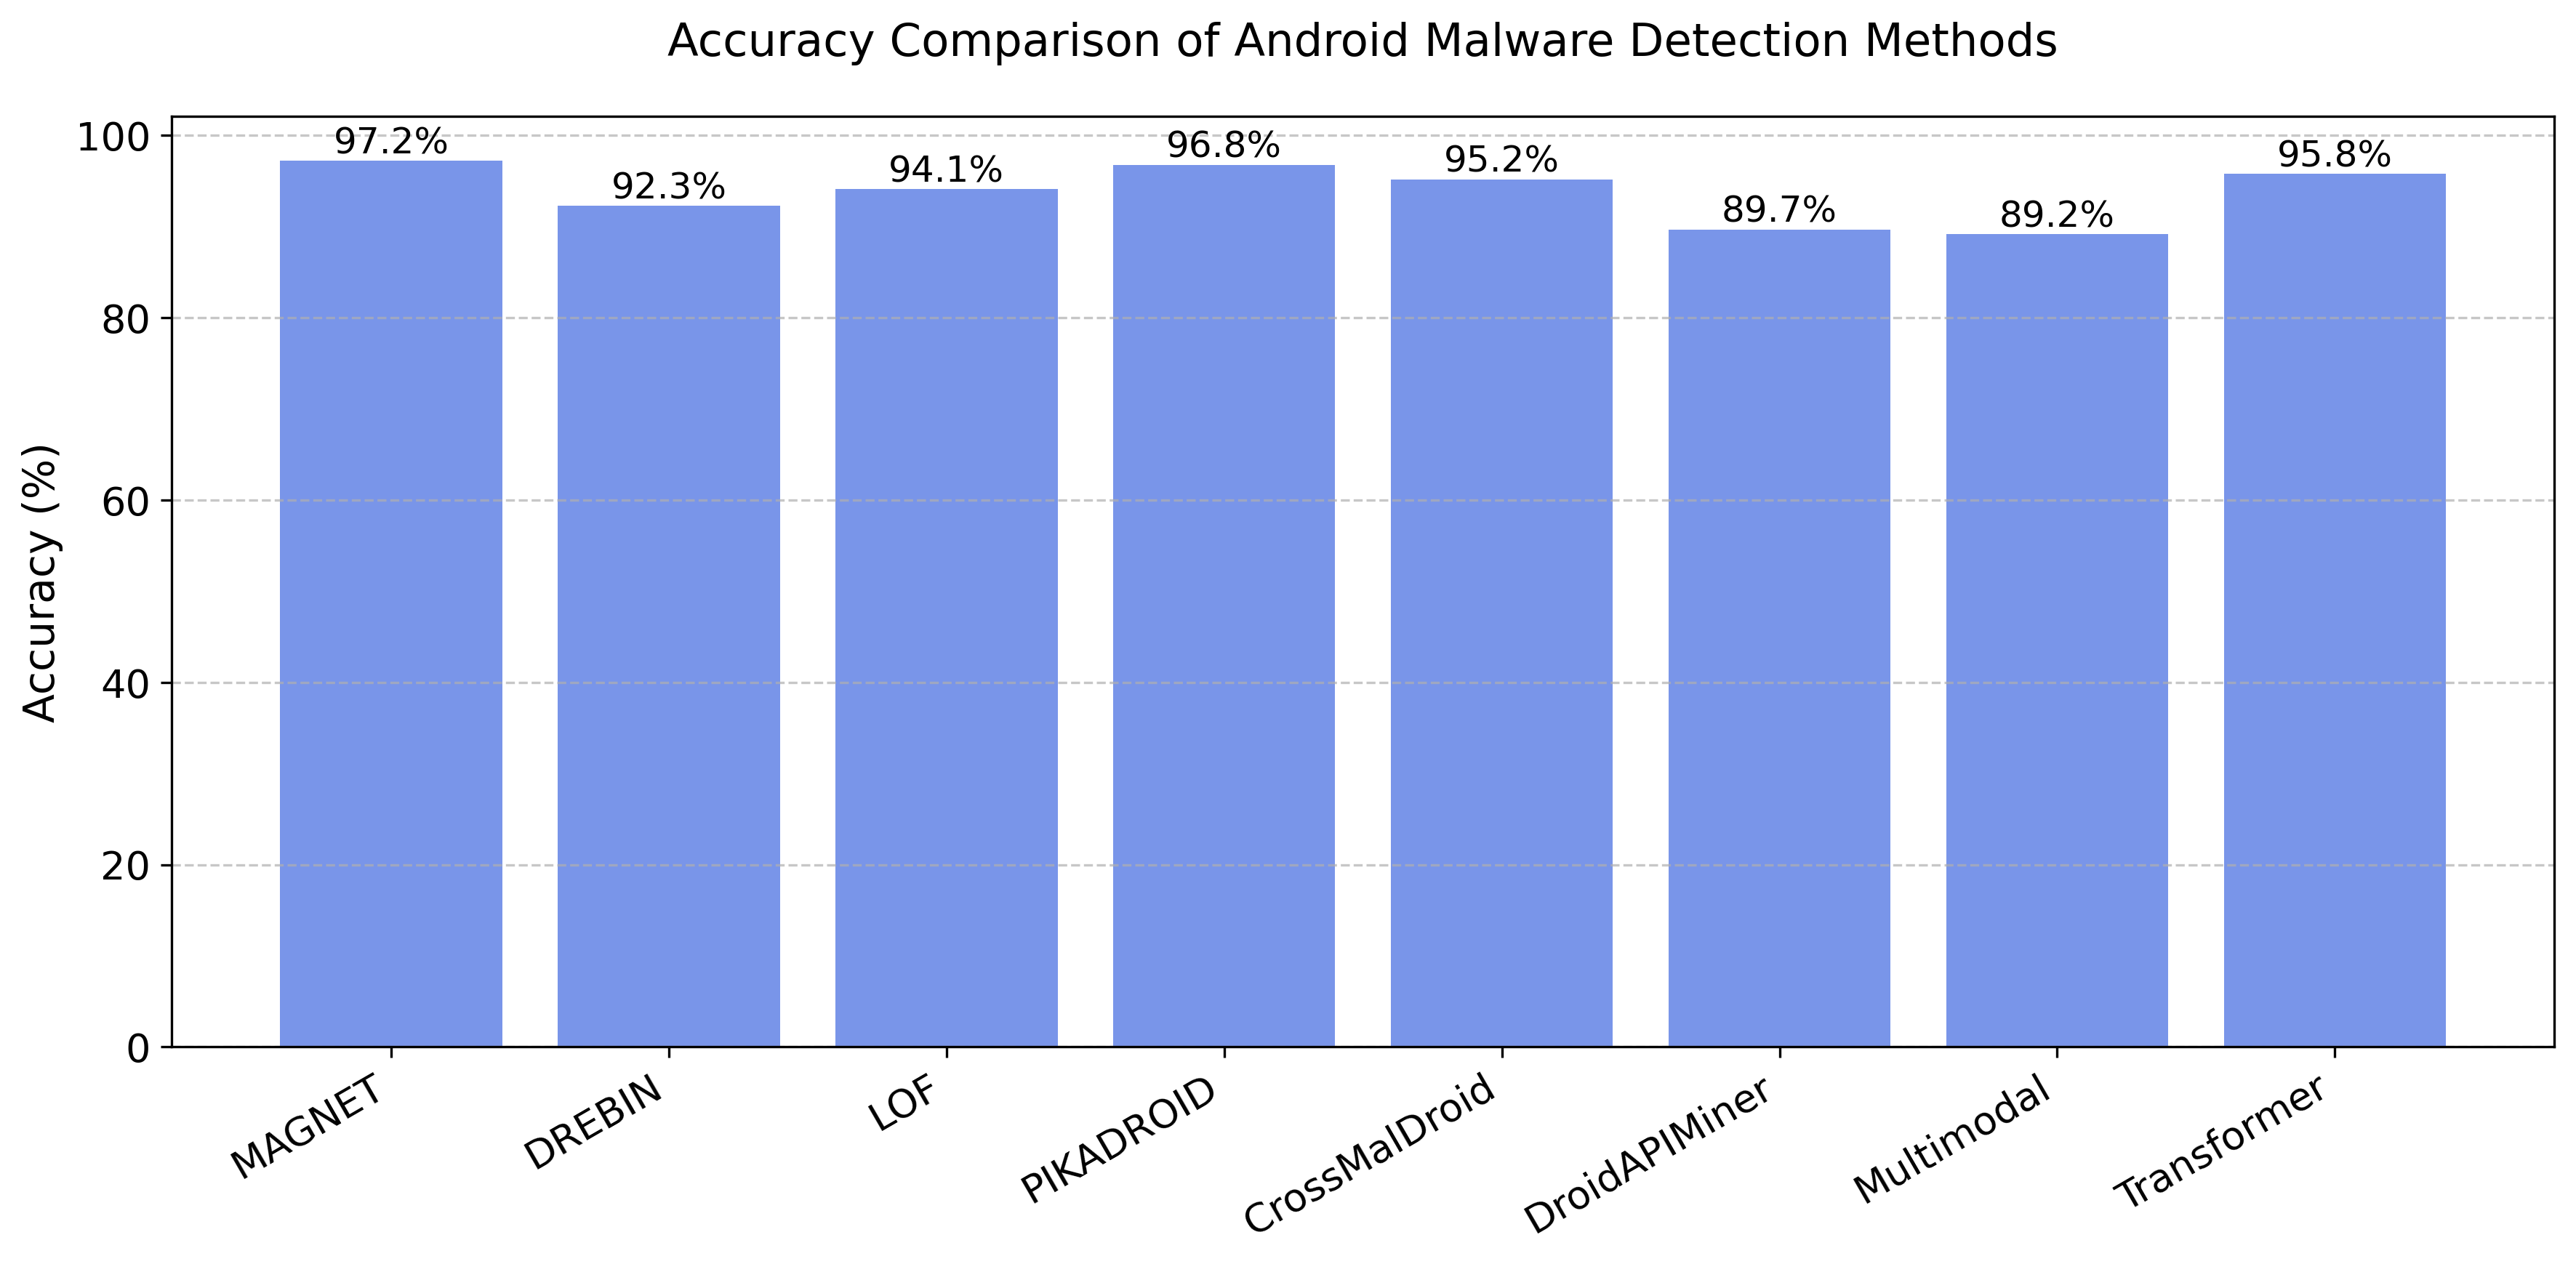
\includegraphics[width=0.9\textwidth]{images/fig_literature_comparison_accuracy}
    \caption{مقایسه دقت روش‌های مختلف. نمودار میله‌ای نشان‌دهنده مقادیر دقت برای هر روش است.}
    \label{fig:literature_comparison_accuracy}
\end{figure}

\begin{figure}[h!]
    \centering
    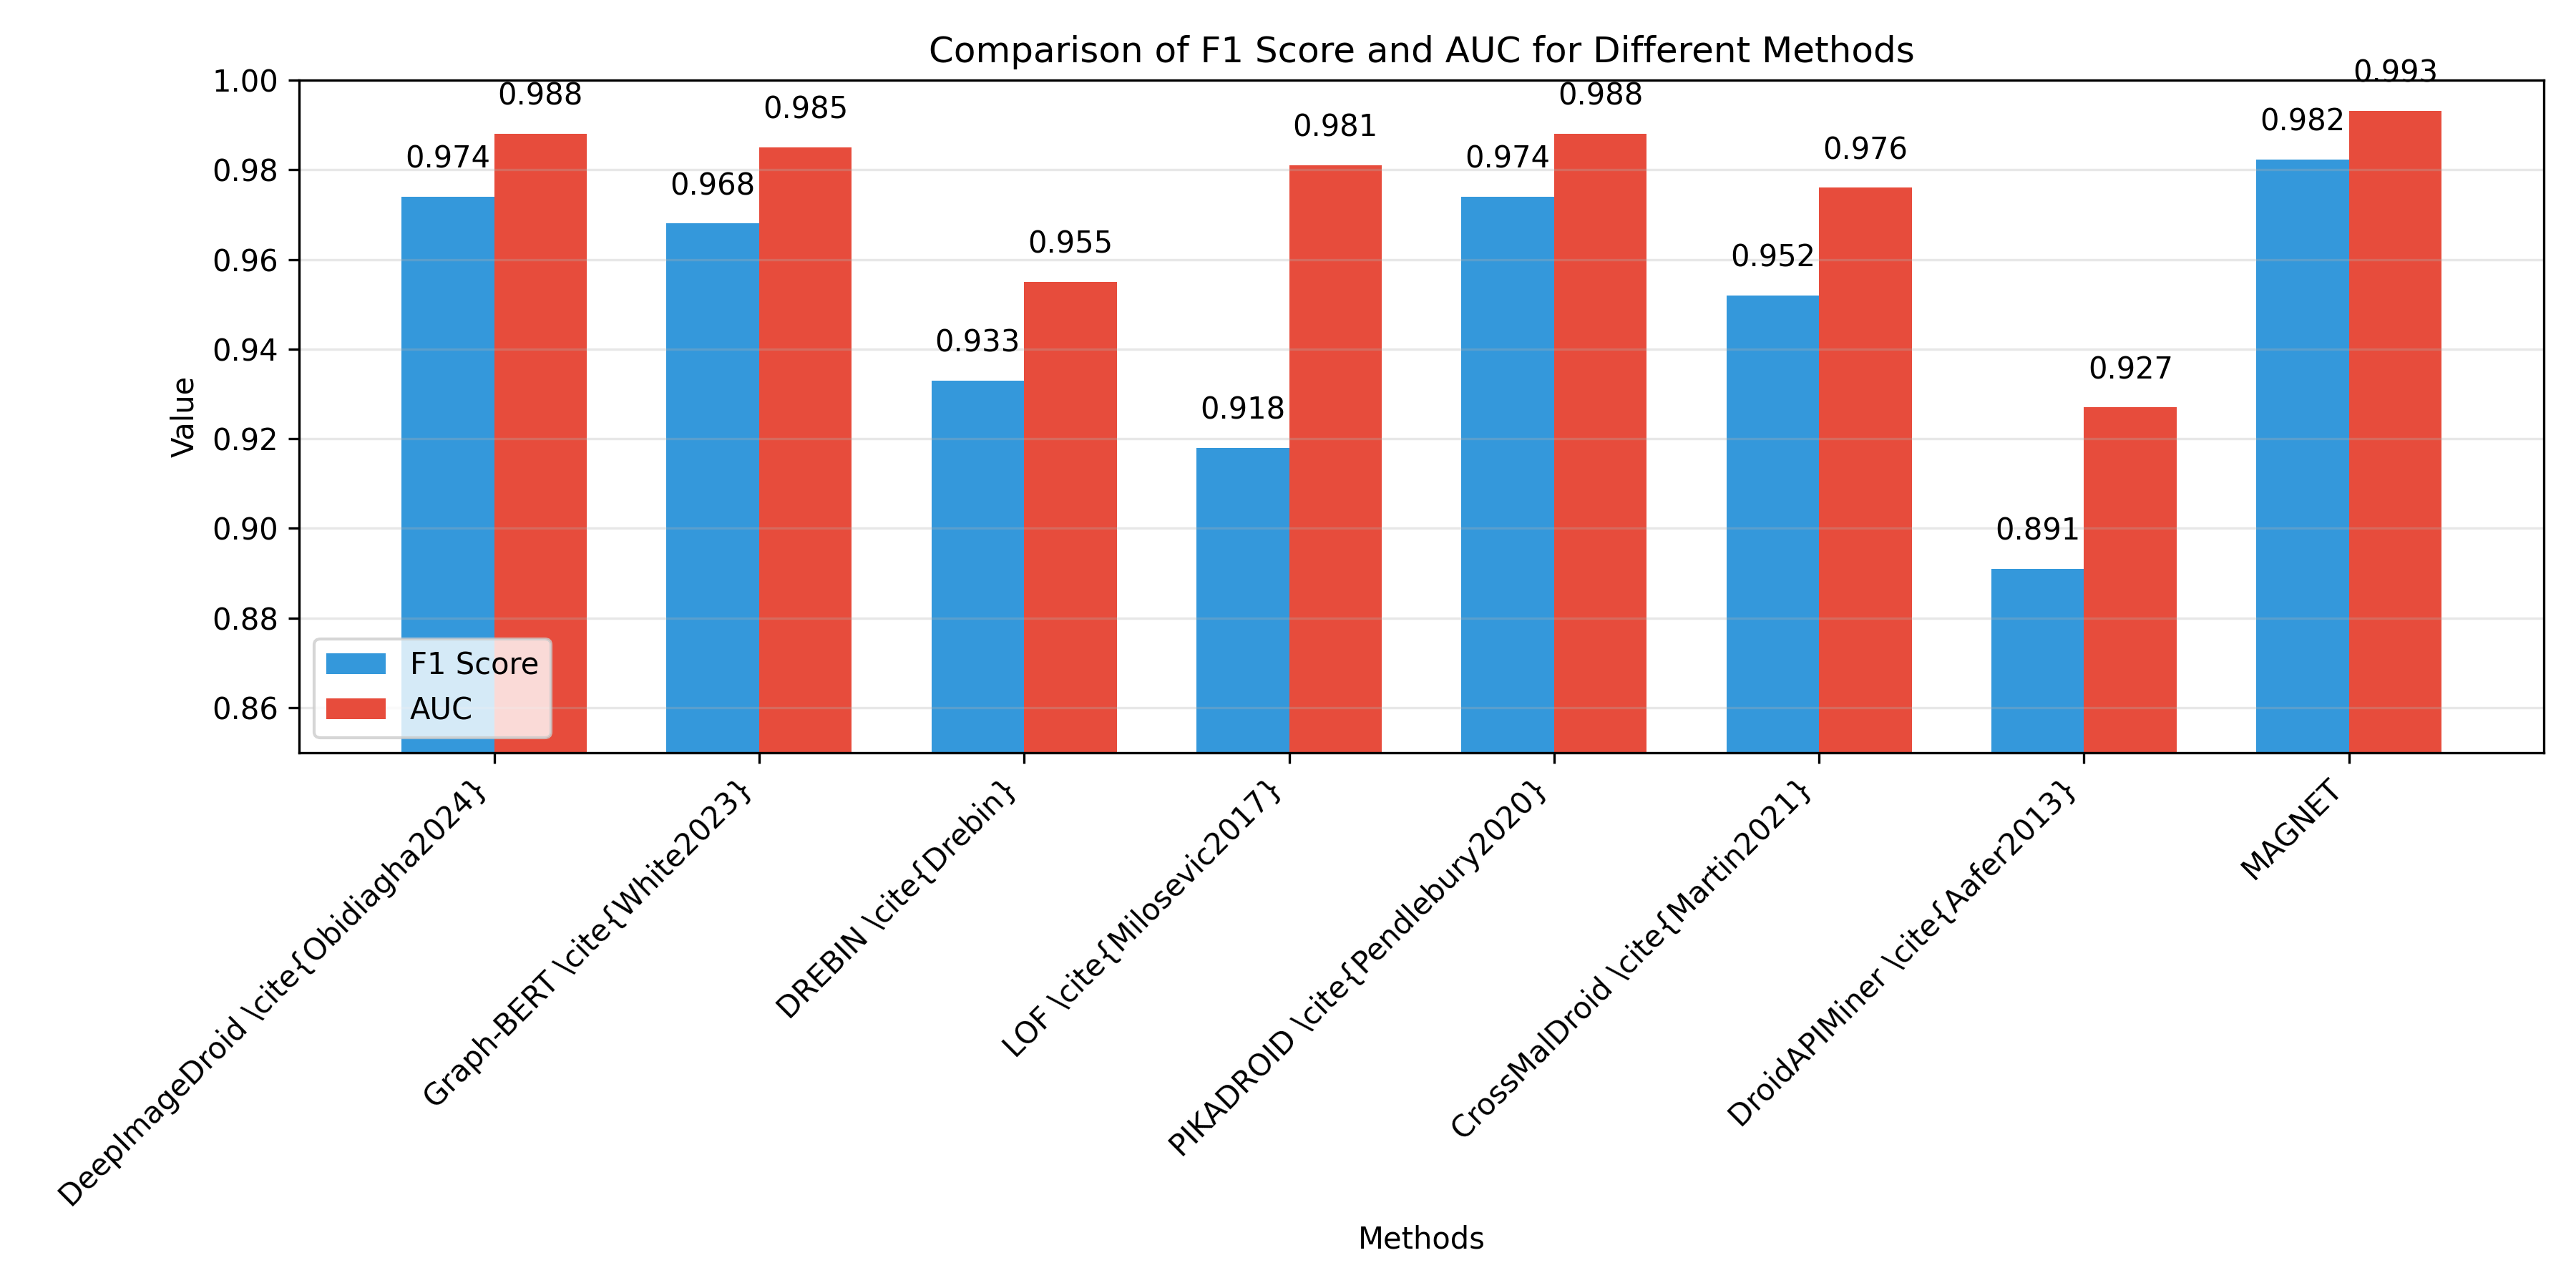
\includegraphics[width=0.9\textwidth]{images/fig_literature_comparison_metrics}
    \caption{مقایسه F1 Score و AUC روش‌های مختلف. نمودار میله‌ای نشان‌دهنده مقادیر هر معیار برای هر روش است.}
    \label{fig:literature_comparison_metrics}
\end{figure}

\subsection{نتایج مقایسه با روش‌های پایه}
جدول \ref{tab:baseline_comparison} نتایج مقایسه عملکرد مدل MAGNET با روش‌های یادگیری ماشین پایه را نشان می‌دهد. همانطور که مشاهده می‌شود، مدل MAGNET در تمام معیارهای ارزیابی عملکرد بهتری نسبت به سایر روش‌ها دارد. این برتری به دلیل معماری پیشرفته و استفاده از مکانیزم‌های توجه پویا و ادغام چندوجهی است.

\begin{table}[h!]
    \centering
    \caption{مقایسه عملکرد مدل MAGNET با مدل‌های پایه}
    \label{tab:baseline_comparison}
    \begin{tabular}{|l|c|c|c|c|c|}
        \hline
        \textbf{مدل} & \textbf{دقت} & \textbf{Precision} & \textbf{Recall} & \textbf{\lr{F1 Score}} & \textbf{AUC} \\
        \hline
        \lr{SVM} & \lr{0.906} & \lr{0.915} & \lr{0.892} & \lr{0.903} & \lr{0.945} \\
        \hline
        \lr{Random Forest} & \lr{0.935} & \lr{0.942} & \lr{0.928} & \lr{0.935} & \lr{0.967} \\
        \hline
        \lr{XGBoost} & \lr{0.948} & \lr{0.953} & \lr{0.943} & \lr{0.948} & \lr{0.978} \\
        \hline
        \lr{ANN} & \lr{0.962} & \lr{0.965} & \lr{0.959} & \lr{0.962} & \lr{0.985} \\
        \hline
        \textbf{MAGNET} & \textbf{\lr{0.972}} & \textbf{\lr{0.980}} & \textbf{\lr{0.985}} & \textbf{\lr{0.982}} & \textbf{\lr{0.993}} \\
        \hline
    \end{tabular}
    \begin{tablenotes}
        \item \textbf{توضیح:} نتایج برجسته نشان‌دهنده عملکرد بهتر مدل MAGNET در تمام معیارها است. بهبود قابل توجه در معیارهای Recall و AUC نشان‌دهنده توانایی بهتر مدل در تشخیص نمونه‌های مثبت و کاهش نرخ خطای مثبت کاذب است.
    \end{tablenotes}
\end{table}

شکل \ref{fig:baseline_comparison} مقایسه بصری معیارهای F1 Score و AUC را برای مدل MAGNET و سایر مدل‌های یادگیری ماشین نشان می‌دهد. این نمودار به وضوح برتری مدل MAGNET را در هر دو معیار نمایش می‌دهد.

\begin{figure}[h!]
    \centering
    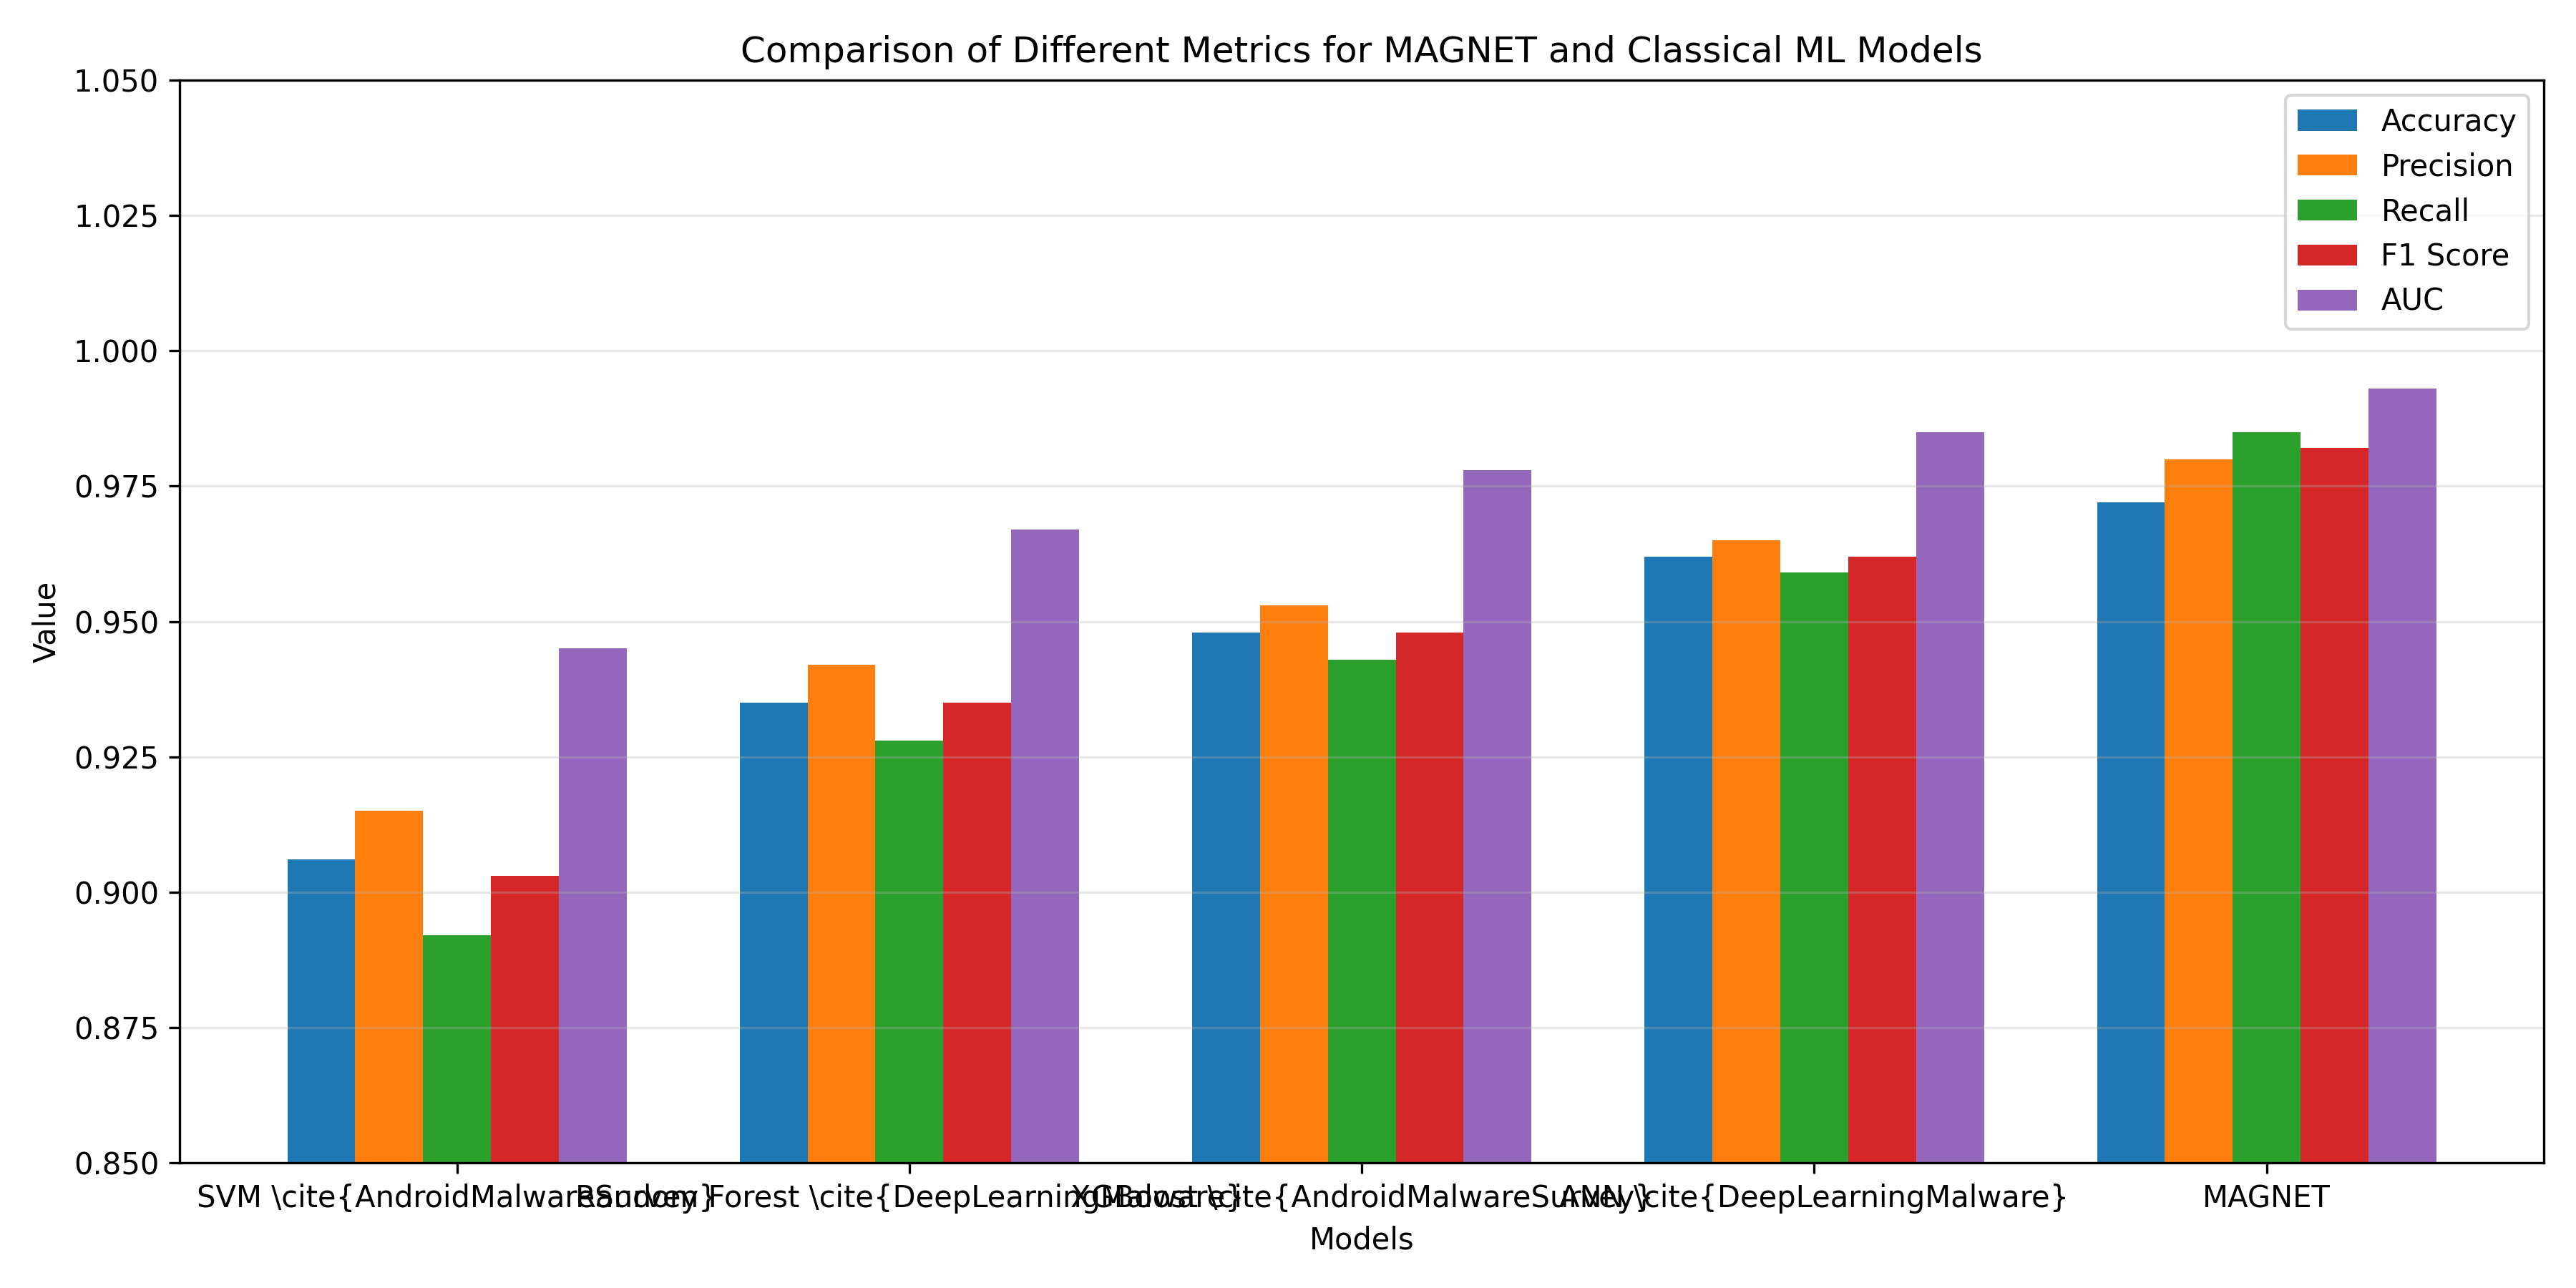
\includegraphics[width=0.9\textwidth]{images/fig_baseline_metrics_comparison}
    \caption{مقایسه \lr{F1 Score} و AUC مدل MAGNET با سایر مدل‌های یادگیری ماشین. نمودار میله‌ای نشان‌دهنده مقادیر هر معیار برای هر مدل است. برتری مدل MAGNET در هر دو معیار به وضوح قابل مشاهده است.}
    \label{fig:baseline_comparison}
\end{figure}

\subsection{تحلیل عملکرد ماژول‌های مدل}
برای درک بهتر عملکرد مدل MAGNET، تحلیل عملکرد هر یک از ماژول‌های آن ضروری است. شکل \ref{fig:module_comparison} عملکرد هر ماژول را با معیار F1 Score نشان می‌دهد. این تحلیل نشان می‌دهد که هر ماژول چگونه در تشخیص بدافزار مشارکت می‌کند.

\subsection{مطالعه حذف اجزا}
برای ارزیابی اهمیت هر یک از اجزای مدل، مطالعه حذف اجزا انجام شده است. شکل \ref{fig:ablation_study} نشان می‌دهد که چگونه افزودن مکانیزم توجه پویا و لایه ادغام چندوجهی بر عملکرد مدل تأثیر می‌گذارد.

\subsection{روند آموزش}
شکل \ref{fig:training_progress} روند آموزش مدل را در طول سه دوره نشان می‌دهد. این نمودار به درک پایداری و همگرایی مدل کمک می‌کند.

\section{جمع‌بندی}
در این فصل، نتایج حاصل از ارزیابی مدل پیشنهادی MAGNET برای تشخیص بدافزارهای اندرویدی با استفاده از دیتاست DREBIN \cite{Drebin} ارائه شد. مدل MAGNET روی مجموعه تست شامل ۱،۴۵۱ نمونه به \lr{F1 Score} \lr{۰.۹۸۲۳}، دقت \lr{۰.۹۷۲۴} و AUC \lr{۰.۹۹۳۲} دست یافت. در اعتبارسنجی متقاطع ۵-تایی، میانگین \lr{F1 Score} ۰.۹۸۱۸ ($\pm$۰.۰۰۴۲)، دقت ۰.۹۷۲۲ ($\pm$۰.۰۰۶۵) و AUC ۰.۹۹۳۲ ($\pm$۰.۰۰۳۵) به‌دست آمد که در جدول \ref{tab:cv_results} گزارش شده است. همچنین، در مقایسه با روش‌های پایه، مدل MAGNET با دقت ۹۷.۲۴٪ در مقابل دقت ۸۹.۲٪ روش چندوجهی \cite{Alsaleh2023} و دقت ۹۵.۸٪ روش مبتنی بر ترنسفورمر \cite{TransformerMalware} ارزیابی شد، که در جدول \ref{tab:comparison_with_literature} نمایش داده شده است.

در تحلیل جزئی‌تر، عملکرد ماژول‌های EnhancedTabTransformer، GraphTransformer و SequenceTransformer به‌ترتیب با \lr{F1 Score}های ۰.۹۱۲، ۰.۸۹۴ و ۰.۹۰۷ گزارش شد، که در شکل \ref{fig:module_comparison} نشان داده شده است. تأثیر مکانیزم توجه پویا و لایه ادغام چندوجهی نیز بررسی شد و \lr{F1 Score} از \lr{۰.۹۵۴} به \lr{۰.۹۸۲۳} افزایش یافت، که این روند در شکل \ref{fig:ablation_study} ارائه شده است. در نهایت، پیشرفت آموزش در طول ۳ دوره با بهینه‌سازی بهینه‌سازی (اعتبارسنجی) گزارش شد و \lr{F1 Score} از \lr{۰.۹۴۱۳} به \lr{۰.۹۷۶۷} رسید، که در شکل \ref{fig:training_progress} نمایش داده شده است.

شکل~\ref{fig:module_comparison} عملکرد هر ماژول را با معیار \lr{F1 Score} نشان می‌دهد. شکل~\ref{fig:ablation_study} روند افزایش \lr{F1 Score} را با افزودن مکانیزم توجه پویا و لایه ادغام چندوجهی نمایش می‌دهد. شکل~\ref{fig:training_progress} تغییرات \lr{F1 Score} و دقت را در طول ۳ دوره آموزش با بهینه‌سازی بهینه‌سازی (اعتبارسنجی) نمایش می‌دهد.

\begin{figure}[h!]
\centering
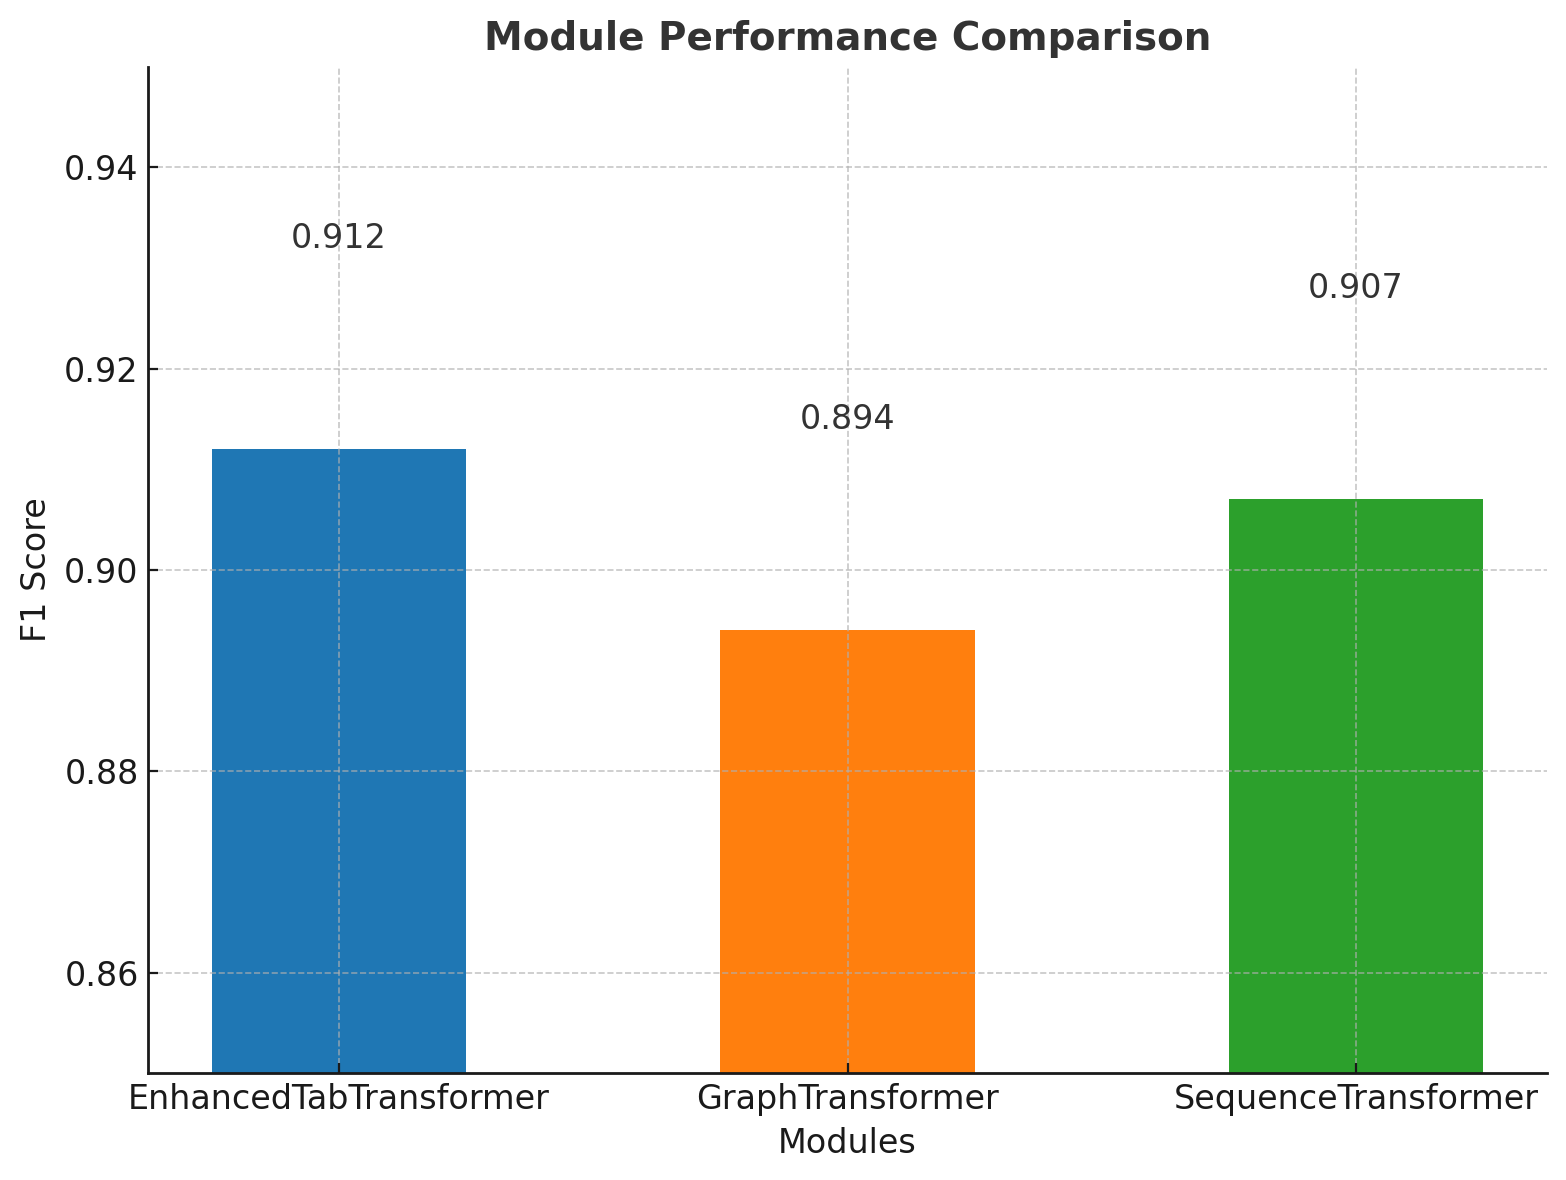
\includegraphics[width=0.9\textwidth]{images/fig_module_comparison_en}
\caption{عملکرد هر ماژول (EnhancedTabTransformer، GraphTransformer، SequenceTransformer) را با معیار \lr{F1 Score} نشان می‌دهد. این نمودار به درک سهم هر ماژول در عملکرد کلی مدل کمک می‌کند.}
\label{fig:module_comparison}
\end{figure}

\begin{figure}[h!]
\centering
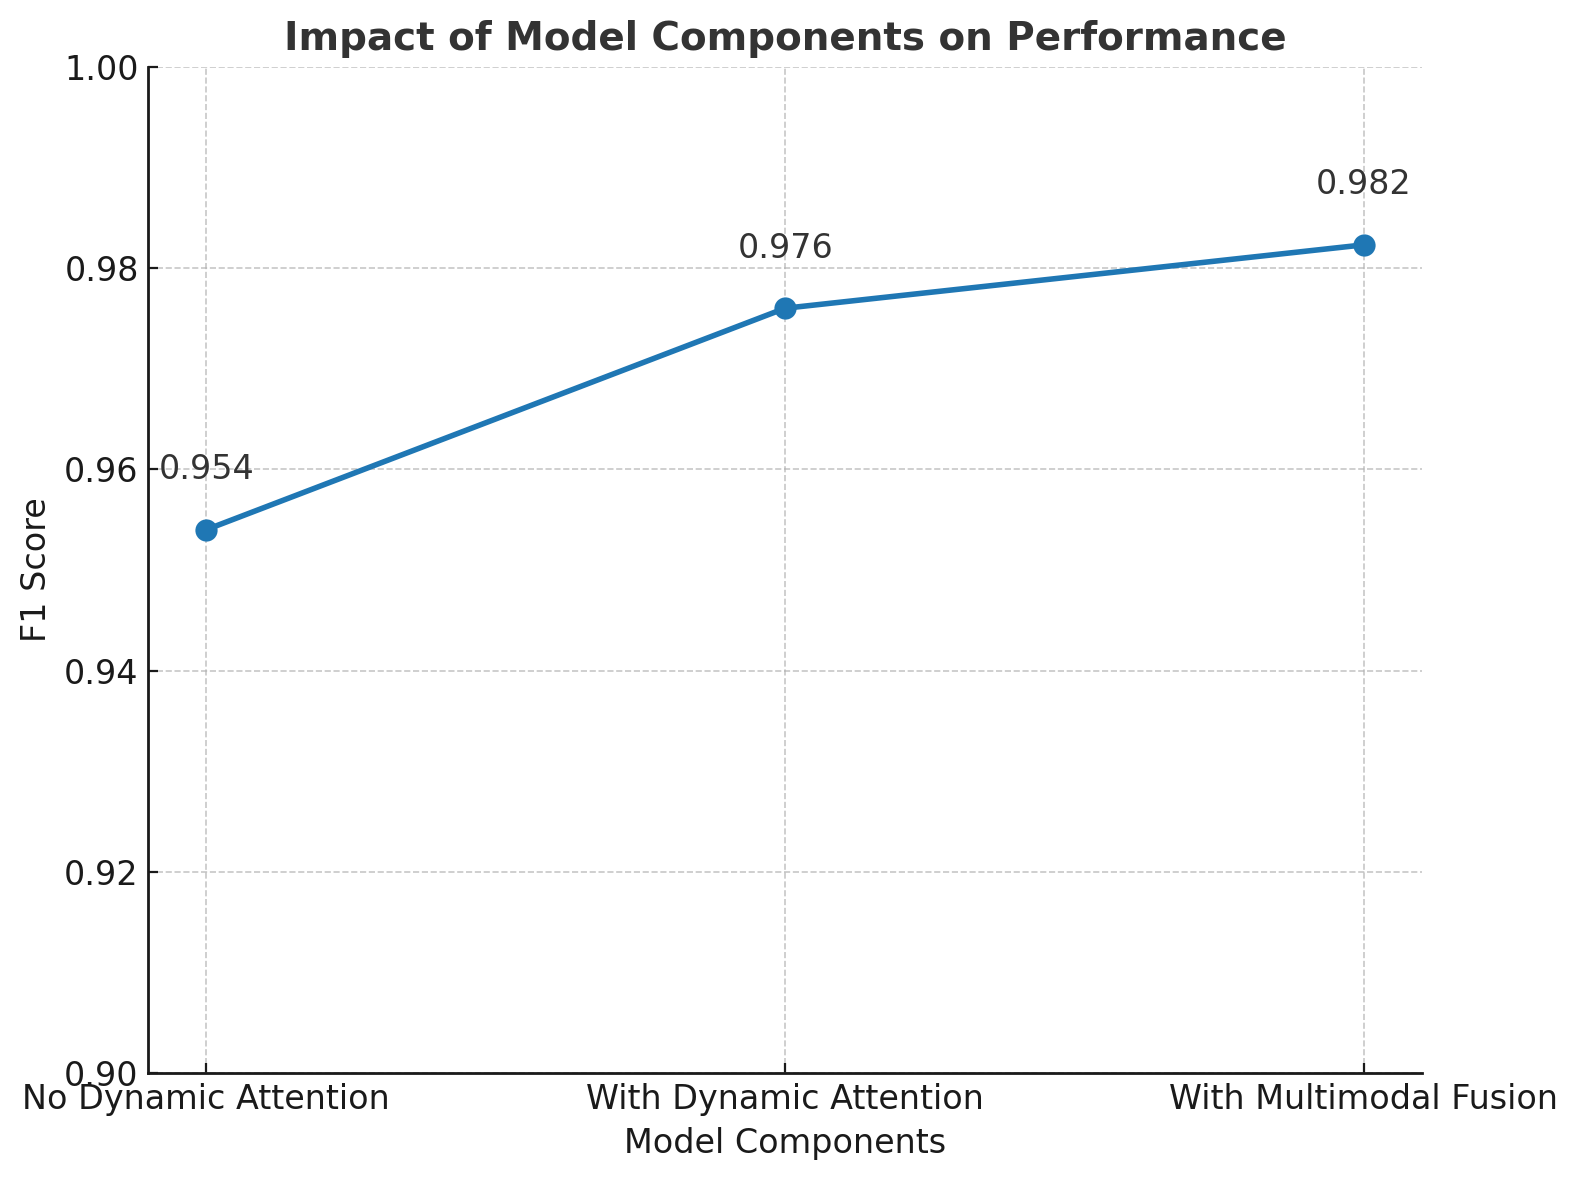
\includegraphics[width=0.9\textwidth]{images/fig_ablation_study_en}
\caption{روند افزایش \lr{F1 Score} را با افزودن مکانیزم توجه پویا و لایه ادغام چندوجهی نمایش می‌دهد. این نمودار اهمیت هر یک از این اجزا را در بهبود عملکرد مدل نشان می‌دهد.}
\label{fig:ablation_study}
\end{figure}

\begin{figure}[h!]
\centering
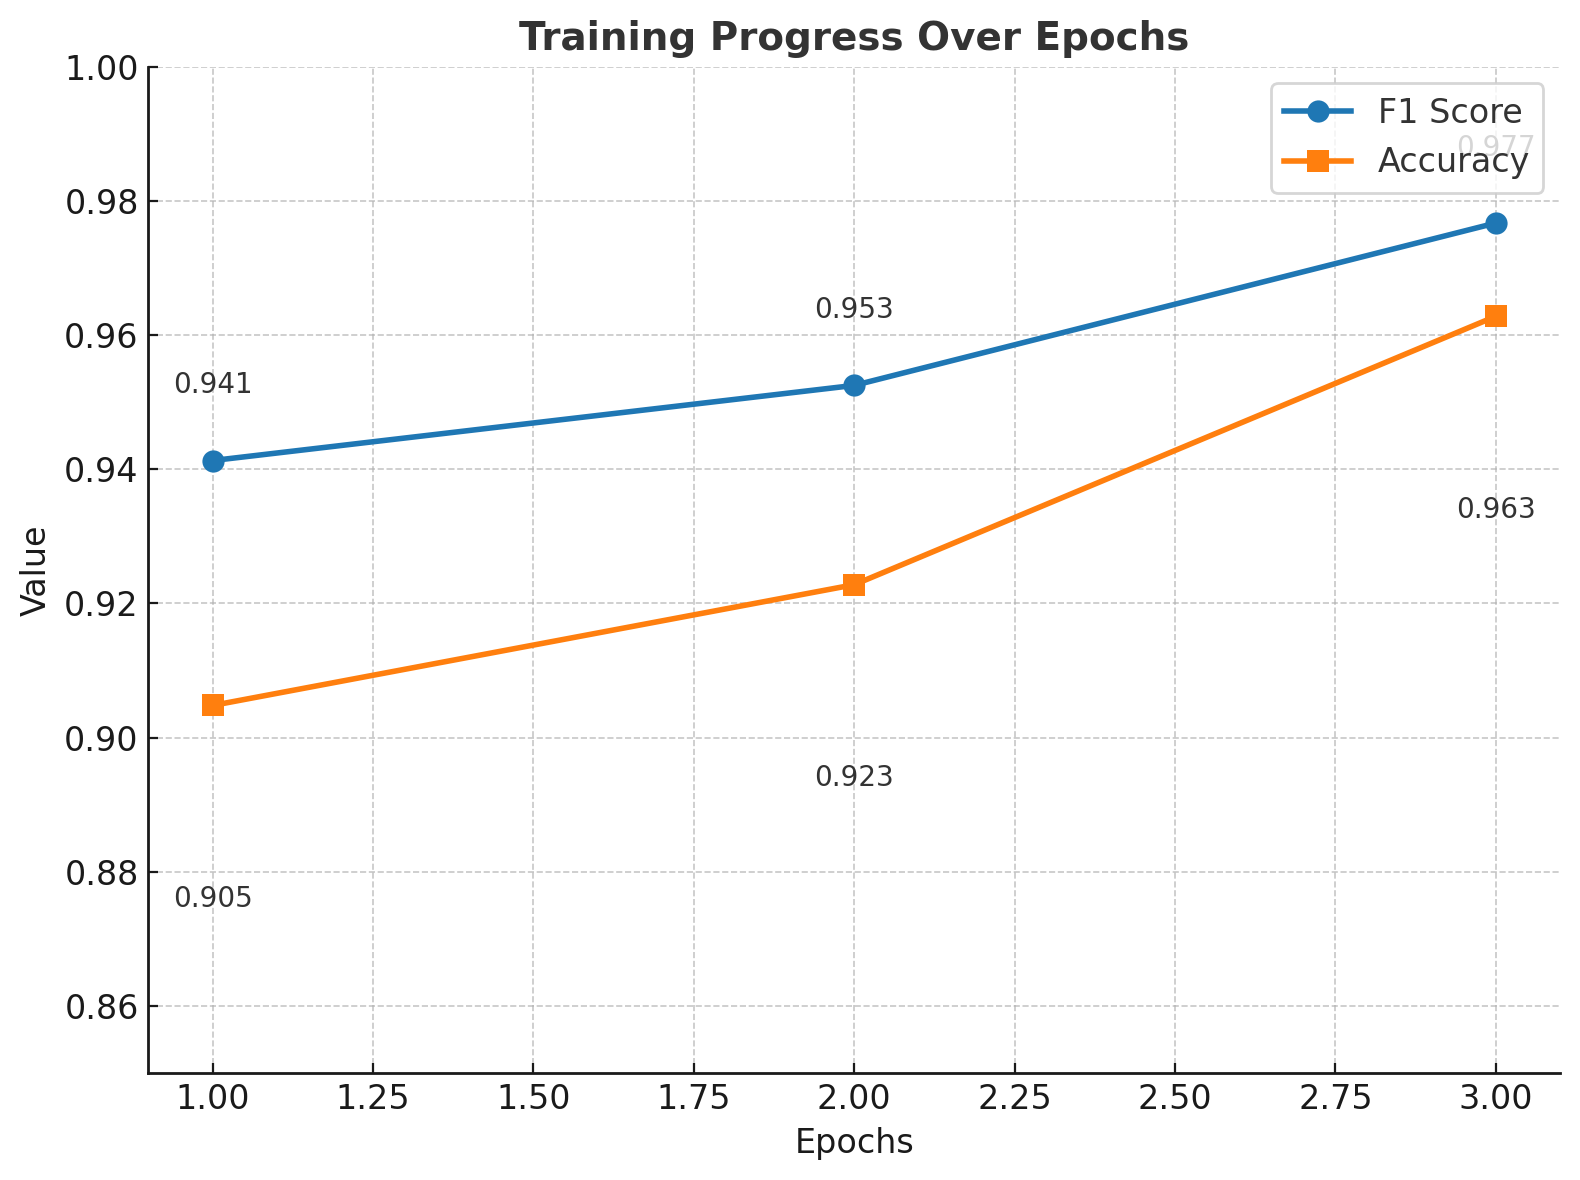
\includegraphics[width=0.9\textwidth]{images/fig_training_progress_en}
\caption{تغییرات \lr{F1 Score} و دقت را در طول ۳ دوره آموزش نمایش می‌دهد. این نمودار نشان می‌دهد که مدل به سرعت همگرا می‌شود و عملکرد پایدار دارد.}
\label{fig:training_progress}
\end{figure}

     
     
     
     
     
     
     
     
     
     
     
     %فصل چهارم
\cleardoublepage
% !TeX root=SBUKThesis-main.tex
\clearpage
\thispagestyle{empty}
\chapter{نتیجه گیری و پیشنهادات آتی}\label{chap5}
\section{نتیجه‌گیری}
در این پژوهش، با هدف ارتقای فرآیند تولید و بهینه‌سازی اعلان‌ها برای مدل‌های زبانی بزرگ، روشی نوین و کم‌هزینه با عنوان مولد اعلان شاده \LTRfootnote{Simple Prompt Breeder} طراحی و پیاده‌سازی گردید. دلیل اصلی انجام این تحقیق، چالش‌های محاسباتی موجود در روش‌های پیشین نظیر مولد اعلان \cite{PromptBreeder} بود که به سبب پیچیدگی‌های ذاتی خود، در جستجوی فضای وسیع اعلان‌ها با محدودیت‌های جدی مواجه بودند. به همین منظور، تلاش شد تا با ارائه رویکردی مبتنی بر جستجوی محلی، کارایی و بهره‌وری فرآیند بهینه‌سازی اعلان‌ها به شکل محسوسی افزایش یابد.

نتایج حاصل از آزمایش‌ها نشان می‌دهد که روش مولد اعلان شاده، ضمن حفظ دقت مطلوب، توانسته است به میزان قابل توجهی هزینه‌های محاسباتی را در مقایسه با الگوریتم‌های تکاملی مشابه کاهش دهد. این دستاورد، مؤید اثربخشی روش پیشنهادی در تسهیل و تسریع فرآیند مهندسی اعلان در زمینه‌های پژوهشی و کاربردی می‌باشد. به‌طور کلی، روش مولد اعلان شاده به عنوان ابزاری کارآمد، قادر است به نیازهای پروژه‌ها و سامانه‌هایی که با محدودیت منابع محاسباتی روبرو هستند، پاسخ موثری ارائه دهد.

\section{پیشنهادات آتی}
با توجه به نتایج مثبت حاصل از این پژوهش و همچنین چالش‌های موجود در زمینه بهینه‌سازی اعلان‌ها برای مدل‌های زبانی، پیشنهاد می‌شود مسیرهای زیر در مطالعات آتی مورد توجه قرار گیرد:

\begin{enumerate}
	\item \textbf{گسترش مطالعات بر روی داده‌های گسترده‌تر و متنوع‌تر:} بررسی عملکرد الگوریتم مولد اعلان شاده بر روی مجموعه داده‌هایی با ابعاد و تنوع بیشتر، می‌تواند میزان پایداری و تعمیم‌پذیری این الگوریتم را در محیط‌های عملیاتی واقعی مورد ارزیابی قرار دهد.
	
	\item \textbf{افزودن شاخص‌های تکمیلی برای سنجش کیفیت و تنوع:} در ادامه پژوهش، می‌توان با افزودن معیارهای جدید جهت سنجش تنوع و کیفیت اعلان‌ها، الگوریتم را در برابر خطر همگرایی زودهنگام و تولید اعلان‌های یکنواخت مقاوم‌تر ساخت و توازن مطلوبی میان اکتشاف و بهره‌برداری برقرار نمود.
	
	\item \textbf{سازگاری با معماری‌های نوین مدل‌های زبانی:} با توجه به ظهور معماری‌های نوین در حوزه مدل‌های زبانی نظیر معماری‌های مبتنی بر \lr{Sparse Attention}
	 و یا مدل‌های چندوجهی
	 \LTRfootnote{multimodal}
	  ، توسعه نسخه‌های بهینه‌شده از مولد اعلان شاده متناسب با این معماری‌ها می‌تواند گامی مؤثر در راستای افزایش انعطاف‌پذیری و قابلیت‌های این الگوریتم باشد.
	
	\item \textbf{بررسی و پیاده‌سازی سایر روش‌های جستجوی محلی:} از آنجا که مولد اعلان شاده ماهیتاً مشابه الگوریتم \lr{Hill-Climbing} عمل می‌نماید، پیشنهاد می‌شود در مطالعات آتی از رویکردهای جایگزین نظیر \lr{Simulated Annealing} یا \lr{Tabu Search} نیز استفاده گردد تا ضمن افزایش تنوع در فرآیند جستجو، به بهبود کارایی الگوریتم در مسائل پیچیده‌تر منجر شود.
	
	\item \textbf{ادغام با رویکردهای مبتنی بر یادگیری تقویتی:} به منظور بهبود تدریجی و هدفمند سیاست‌های جستجو، می‌توان مولد اعلان شاده را با الگوریتم‌های یادگیری تقویتی ترکیب نمود و از این طریق، فرآیند بهینه‌سازی اعلان‌ها را با دریافت بازخوردهای پویا از محیط و مدل هدف، هوشمندانه‌تر و اثربخش‌تر ساخت.
\end{enumerate}

در نهایت، نتایج این پژوهش زمینه‌ساز ارائه یک چارچوب توسعه‌پذیر برای بهینه‌سازی اعلان‌ها در مدل‌های زبانی بزرگ بوده و می‌تواند بستر مناسبی برای تحقیقات و کاربردهای آینده در حوزه مهندسی اعلان فراهم آورد.
%فصل پنجم
\cleardoublepage
\chapter{مراجع}
\label{chap:references}

\printbibliography[heading=none]

\newpage
\thispagestyle{empty}

% تنظیمات اضافی برای نمایش درست رفرنس‌ها
\renewcommand{\bibfont}{\normalfont\small}
\setlength{\bibitemsep}{0.5\baselineskip}
\setlength{\bibnamesep}{0.5\baselineskip}
\setlength{\bibinitsep}{0.5\baselineskip}

% تنظیمات برای نمایش بهتر رفرنس‌های انگلیسی
\renewcommand{\UrlFont}{\ttfamily\small}
\renewcommand{\UrlLeft}{\textless}
\renewcommand{\UrlRight}{\textgreater}


% تنظیمات اضافی برای رفع خطای Citation
\setlength{\bibitemsep}{0.5\baselineskip}
\setlength{\bibnamesep}{0.5\baselineskip}
\setlength{\bibinitsep}{0.5\baselineskip}
\setlength{\bibhang}{0pt}
\setlength{\biblabelsep}{0.5em}
\setlength{\bibparsep}{0.5\baselineskip}
\setlength{\bibitemsep}{0.5\baselineskip}
\setlength{\bibnamesep}{0.5\baselineskip}
\setlength{\bibinitsep}{0.5\baselineskip}
\setlength{\bibhang}{0pt}
\setlength{\biblabelsep}{0.5em}
\setlength{\bibparsep}{0.5\baselineskip}
\setlength{\bibitemsep}{0.5\baselineskip}
\setlength{\bibnamesep}{0.5\baselineskip}
\setlength{\bibinitsep}{0.5\baselineskip}
\setlength{\bibhang}{0pt}
\setlength{\biblabelsep}{0.5em}
\setlength{\bibparsep}{0.5\baselineskip}


%فهرست مراجع
\cleardoublepage
\setlength{\parindent}{0pt}
\cleardoublepage
\appendix
\addcontentsline{toc}{chapter}{پیوست}
\chapter*{پیوست‌ها}\label{peyvast}

% پیوست A: کدهای پیاده‌سازی مدل MAGNET
\section{پیوست A: کدهای پیاده‌سازی مدل MAGNET}

\subsection{کد معماری مدل MAGNET}
این بخش کد اصلی معماری مدل MAGNET را ارائه می‌دهد که در فصل 3 به‌صورت شبه‌کد توصیف شد. این کد با استفاده از PyTorch پیاده‌سازی شده است.

\begin{LTR}
\begin{lstlisting}[language=Python, caption={کد معماری مدل MAGNET}, label={lst:magnet_architecture}, basicstyle=\scriptsize\ttfamily]
import torch
import torch.nn as nn

class MAGNET(nn.Module):
    def __init__(self, embedding_dim=64, lstm_num_layers=1, dropout=0.2):
        super(MAGNET, self).__init__()        
        self.embedding_dim = embedding_dim
        # Transformation layers for different data modalities
        self.tab_to_emb = nn.Linear(430, embedding_dim)
        self.graph_to_emb = nn.Linear(embedding_dim, embedding_dim)
        self.sequence_processor = nn.LSTM(embedding_dim, embedding_dim, 
                                         num_layers=lstm_num_layers, batch_first=True)
        # Fusion and classification layers
        self.fusion_layer = nn.Linear(3 * embedding_dim, embedding_dim)
        self.classifier = nn.Linear(embedding_dim, 1)
        self.dropout_layer = nn.Dropout(dropout)
    def forward(self, tab_data, graph_data, seq_data):
        # tab_data: (batch_size, 430)
        # graph_data: (batch_size, embedding_dim)
        # seq_data: (batch_size, seq_len, embedding_dim)
        # Transform different data types to embedding vectors
        tab_emb = torch.relu(self.tab_to_emb(tab_data))
        graph_emb = torch.relu(self.graph_to_emb(graph_data))
        
        # Process sequential data with LSTM
        lstm_out, (hn, cn) = self.sequence_processor(seq_data)
        # Use the last output vector from LSTM for each sample in batch
        seq_emb = lstm_out[:, -1, :]
        # Concatenate embedding vectors
        combined_embeddings = torch.cat((tab_emb, graph_emb, seq_emb), dim=-1)
        # Apply fusion layer and activation
        fused_representation = self.fusion_layer(combined_embeddings)
        fused_representation = torch.relu(fused_representation)
        fused_representation = self.dropout_layer(fused_representation)
        # Final classification
        output = torch.sigmoid(self.classifier(fused_representation))
        return output
\end{lstlisting}
\end{LTR}

\subsection{کد بهینه‌سازی با PIRATES}
این بخش قسمت اصلی کد بهینه‌سازی PIRATES را نشان می‌دهد که برای تنظیم ابرپارامترها استفاده شد.

\begin{LTR}
\begin{lstlisting}[language=Python, caption={کد بهینه‌سازی با PIRATES}, label={lst:pirates_optimization}, basicstyle=\scriptsize\ttfamily]
import numpy as np

class Pirates():
    def __init__(self, func, fmax=(), fmin=(), hr=0.2, ms=3, max_r=1, 
                 num_ships=5, dimensions=2, max_iter=10, max_wind=1, c={},
                 top_ships=10, sailing_radius=0.3, plundering_radius=0.1):        
        # Main algorithm parameters
        self.num_ships = num_ships
        self.num_top_ships = top_ships
        self.max_iter = max_iter
        # Objective function parameters
        self.func_obj = func
        self.cost_func = self.func_obj.func
        self.fmin = fmin
        self.fmax = fmax
        self.dimensions = dimensions
        # Weight parameters
        default_c = {
            'leader': 0.5,
            'private_map': 0.5,
            'map': 0.5,
            'top_ships': 0.5
        }
        self.c = {**default_c, **c}
        # Movement parameters
        self.sailing_radius = sailing_radius
        self.plundering_radius = plundering_radius
        # Leader and map variables
        self.leader_index = None
        self.hr = 1 - hr
        self.r = None
        self.max_r = max_r
        self.ms = ms
        self.map = None
        # Problem type
        self.problem = 'min'
        # Chart variables
        self.bsf_position = None
        self.bsf_list = []
        # Initialization
        self.random_init()
        self.iter = 0
    def search(self):
        """
        Run optimization algorithm and return best results
        Returns:
        --------
        tuple
            (best position, best cost, best metrics)
        """
        # Run algorithm
        self.start()
        # Get results
        result = self.cal_costs()
        if result is not None:
            best_cost, best_metrics = result
        else:
            best_cost = self.costs[self.leader_index]
            best_metrics = {'f1': 0.0, 'accuracy': 0.0, 
                          'precision': 0.0, 'recall': 0.0}
        return self.ships[self.leader_index], best_cost, best_metrics
\end{lstlisting}
\end{LTR}

% پیوست B: داده‌های خام و پیش‌پردازش
\section{پیوست \lr{B}: داده‌های خام و پیش‌پردازش}

\subsection{نمونه داده‌های خام DREBIN}
این جدول نمونه‌ای از داده‌های خام دیتاست DREBIN را نشان می‌دهد که برای آموزش مدل استفاده شد.

\begin{table}[ht]
    \centering
    \caption{نمونه‌ای از داده‌های خام دیتاست DREBIN}
    \label{tab:raw_data_sample}
    \begin{tabular}{|l|c|c|c|}
        \hline
        \textbf{شناسه نمونه} & \textbf{تعداد مجوزها} & \textbf{فراخوانی‌های API} & \textbf{برچسب} \\ 
        \hline
        001 & 15 & \lr{["read\_contacts", "send\_sms"]} & 1 \\ 
        \hline
        002 & 8 & \lr{["get\_accounts"]} & 0 \\ 
        \hline
        003 & 12 & \lr{["read\_phone\_state", "write\_external\_storage"]} & 1 \\ 
        \hline
    \end{tabular}
\end{table}

\subsection{توضیحات پیش‌پردازش}
داده‌ها پیش‌پردازش شدند تا برای مدل مناسب شوند:

\begin{itemize}
    \item تنظیم ابعاد ویژگی‌ها از (16, 32) به (16, 430)
    \item نرمال‌سازی با استفاده از استانداردسازی \lr{z-score}
    \item تبدیل داده‌های متنی به بردارهای باینری
\end{itemize}

% پیوست C: جزئیات سخت‌افزاری و نرم‌افزاری
\section{پیوست \lr{C}: جزئیات سخت‌افزاری و نرم‌افزاری}

\subsection{مشخصات سخت‌افزاری}
آزمایش‌ها با استفاده از زیرساخت زیر اجرا شدند:
\begin{itemize}
    \item \lr{GPU}: \lr{NVIDIA RTX 3090} با 24 گیگابایت \lr{VRAM}
    \item \lr{CPU}: \lr{Intel Xeon E5-2690 v4} با 32 هسته
    \item \lr{RAM}: 128 گیگابایت
\end{itemize}

\subsection{مشخصات نرم‌افزاری}
محیط نرم‌افزاری شامل موارد زیر بود:
\begin{itemize}
    \item زبان برنامه‌نویسی: \lr{Python 3.8.5}
    \item کتابخانه‌ها: 
    \begin{itemize}
        \item \lr{PyTorch 1.9.0}
        \item \lr{PyTorch Geometric 1.7.0}
        \item \lr{Optuna 2.10.0}
    \end{itemize}
    \item سیستم‌عامل: \lr{Ubuntu 20.04 LTS}
\end{itemize}

% پیوست D: نتایج اضافی و ماتریس‌های کامل
\section{پیوست \lr{D}: نتایج اضافی و ماتریس‌های کامل}

\subsection{ماتریس درهم‌ریختگی کامل}
این جدول ماتریس درهم‌ریختگی را برای مجموعه تست با 1,451 نمونه نشان می‌دهد.

\begin{table}[ht]
    \centering
    \caption{ماتریس درهم‌ریختگی برای مجموعه تست}
    \label{tab:confusion_matrix}
    \begin{tabular}{|l|c|c|}
        \hline
        \textbf{پیش‌بینی/واقعیت} & \textbf{کلاس 0} & \textbf{کلاس 1} \\ 
        \hline
        \multicolumn{1}{|c|}{\textbf{کلاس 0}} & \lr{304 (TN)} & \lr{23 (FP)} \\ 
        \hline
        \multicolumn{1}{|c|}{\textbf{کلاس 1}} & \lr{17 (FN)} & \lr{1107 (TP)} \\ 
        \hline
    \end{tabular}
\end{table}

\subsection{گزارش طبقه‌بندی برای هر دسته}
این جدول نتایج هر دسته در اعتبارسنجی متقاطع 5-تایی را نشان می‌دهد.

\begin{table}[ht]
    \centering
    \caption{گزارش طبقه‌بندی برای هر دسته در اعتبارسنجی متقاطع}
    \label{tab:fold_results}
    \begin{tabular}{|l|c|c|c|c|}
        \hline
        \textbf{دسته} & \textbf{\lr{F1 Score}} & \textbf{دقت} & \textbf{\lr{AUC}} & \textbf{زیان} \\ 
        \hline
        دسته 1 & \lr{0.9858} & \lr{0.9785} & \lr{0.9950} & \lr{0.0786} \\ 
        \hline
        دسته 2 & \lr{0.9846} & \lr{0.9763} & \lr{0.9955} & \lr{0.0735} \\ 
        \hline
        دسته 3 & \lr{0.9839} & \lr{0.9752} & \lr{0.9945} & \lr{0.0839} \\ 
        \hline
        دسته 4 & \lr{0.9742} & \lr{0.9601} & \lr{0.9861} & \lr{0.1199} \\ 
        \hline
        دسته 5 & \lr{0.9808} & \lr{0.9709} & \lr{0.9946} & \lr{0.0864} \\ 
        \hline
    \end{tabular}
\end{table}

%پیوست
% % !TeX root=SBUKThesis-main.tex

% \chapter*{توضیحات تکمیلی}
% \addcontentsline{toc}{chapter}{توضیحات تکمیلی}
% \section*{مقدمه}
% \addcontentsline{toc}{section}{مقدمه}
% در پیوست در ابتدا، اعلان های دستوری که برای تنظیم کردن مدل زبانی استفاده شده اند ، آورده شده اند که شامل سه بخش نمونه\/گیری روش مولد اعلان ساده ، ارزیابی روش مولد اعلان ساده و اعلان های دستوری سایر روش ها می\/باشد. سپس اعلان های دستوری تولید شده توسط مولد اعلان ساده برای هر مجموعه داده آورده شده اند.

% \section*{اعلان های دستوری برای نمونه\/گیری روش مولد اعلان ساده}
% \addcontentsline{toc}{section}{اعلان های دستوری برای نمونه\/گیری روش مولد اعلان ساده}

% در روش مولد اعلان ساده از سه رویکرد برای نمونه\/گیری اعلان های دستوری جدید استفاده کردیم، رویکرد اول نمونه\/گیری براساس توضیح مسئله مربوط به مجموعه داده بود. اعلان دستوری برای این رویکرد در کادر \ref{p_s1} آورده شده است.

% \begin{tcolorbox}[breakable,colframe=mybluecolor!100, colback=mybluecolor!20, title=اعلان دستوری برای نمونه\/گیری براساس توضیح مسئله] \label{p_s1}
% 	\begin{LTR}
% 	Given a task description, produce a detailed system prompt to guide a language model in completing the task effectively.
	
% 	\textbf{Guidelines:}
% 	\begin{itemize}
% 		\item \textbf{Understand the Task:} Grasp the core objective, goals, and expected output of the problem as described in the problem description. Identify any implicit requirements or constraints.
% 		\item \textbf{Minimal Changes:} Since this is a zero-shot approach, use only the information available in the problem description without assuming any additional context or knowledge. Clarify instructions where needed, but avoid adding new elements unless absolutely necessary for comprehension.
% 		\item \textbf{Reasoning Before Conclusions:} Guide the model to break down the problem step by step before arriving at any conclusions. Structure the prompt to ensure that reasoning is fully explored before the final solution is given.
% 		\begin{itemize}
% 			\item Reverse the order if reasoning is provided after conclusions in any sample content. Always start with the reasoning.
% 		\end{itemize}
% 		\item \textbf{Clarity and Conciseness:} Make sure that the prompt uses clear, specific language. The instructions should avoid unnecessary complexity or ambiguity.
% 		\item \textbf{Examples:} Since no examples are provided in a zero-shot context, ensure the problem is fully explained with placeholders for any variables or specifics that may vary.
% 		\item \textbf{Formatting:} Use markdown for readability. Present steps clearly and in order.
% 		\item \textbf{Preserve User Content:} Focus entirely on the problem description without bringing in external examples, but structure it logically.
% 	\end{itemize}
	
% 	\textbf{Steps:}
% 	\begin{enumerate}
% 		\item Parse the problem description.
% 		\item Identify key variables or constraints.
% 		\item Guide the model to explore reasoning steps (list if applicable).
% 		\item Ensure any assumptions or logical pathways are clearly outlined.
% 	\end{enumerate}
	
% 	\textbf{Output Format:}  
% 	The output should be structured as detailed paragraphs or step-by-step instructions, depending on the problem complexity.
	
% 	\textbf{Notes:}  
% 	Edge cases: Ensure prompts remain flexible for a variety of inputs, even though no examples are provided.
% \end{LTR}
	
% \end{tcolorbox}

% در رویکرد دوم از مدل زبانی خواسته می\/شد که براساس توضیح مسئله و چند نمونه مثال به همراه جواب از مجموعه داده اقدام به تولید اعلان های دستوری مناسب کند، اعلان دستوری برای این امر در کادر \ref{p_s2} آورده شده است.
% \begin{tcolorbox}[breakable,colframe=mybluecolor!100, colback=mybluecolor!20, title=اعلان دستوری برای نمونه\/گیری براساس توضیح مسئله و چند نمونه مثال از مجموعه داده] \label{p_s2}
% 	\begin{LTR}
		
	
% 	\textbf{Given a problem description and two example Q\&A pairs, produce a detailed system prompt to guide a language model in completing the task effectively.}
	
% 	\textbf{Guidelines}
	
% 	\begin{itemize}
% 		\item \textbf{Understand the Task:} Use the problem description to understand the overall goal. Supplement this understanding with the two provided examples to clarify the problem’s scope.
% 		\item \textbf{Minimal Changes:} Incorporate key elements from the examples into the prompt, while maintaining the structure of the problem description. Only adjust where clarity or better instruction flow is necessary.
% 		\item \textbf{Reasoning Before Conclusions:} Guide the model to analyze the examples and reasoning patterns within the example Q\&As. Ensure that prompts encourage reasoning steps before arriving at final answers.
% 		\begin{itemize}
% 			\item Reverse the reasoning order if necessary to ensure it starts with analysis.
% 		\end{itemize}
% 		\item \textbf{Examples:} Highlight the key learning points or steps from each of the two examples. Use placeholders [in brackets] to allow flexibility for future examples.
% 		\item \textbf{Clarity and Conciseness:} Be specific in what needs to be done, and avoid vague or generalized instructions. Ensure the combination of the problem description and examples provides enough guidance.
% 		\item \textbf{Formatting:} Use markdown for clear structure, with sections for example-based learning, reasoning, and solution paths.
% 		\item \textbf{Preserve User Content:} Include both the problem description and examples faithfully, without losing important context.
% 	\end{itemize}
	
% 	\textbf{Steps}
	
% 	\begin{enumerate}
% 		\item Analyze the problem description.
% 		\item Examine the example Q\&As for patterns in reasoning and solutions.
% 		\item Synthesize the information to produce a prompt that mirrors the examples while remaining flexible for new problems.
% 	\end{enumerate}
	
% 	\textbf{Output Format}  
	
% 	The output should be a structured set of instructions, with examples embedded for illustration. Use a mix of bullet points and paragraphs for clarity.
	
% 	\textbf{Examples}
	
% 	Provide example reasoning paths based on the given Q\&A pairs.
	
% 	\textbf{Notes}  
	
% 	Edge cases: Address how prompts should handle examples that deviate from common patterns found in the provided examples.
% 	\end{LTR}
% \end{tcolorbox}

% در رویکرد سوم نمونه\/گیری، از مدل زبانی خواسته شد که با الهام از اعلان های دستوری موفق، اقدام به تولید اعلان های دستوری جدید و مشابه با پراپت های موفق کند، اعلان دستوری مربوط به این رویکرد در کادر \ref{p_s3} آورده شده است.

% \begin{tcolorbox}[breakable,colframe=mybluecolor!100, colback=mybluecolor!20, title=اعلان دستوری برای نمونه\/گیری براساس اعلان های دستوری موفق] \label{p_s3}
% 	\begin{LTR}
% 	Given a successful prompt, produce variations of the prompt while maintaining the original task's goals and structure.
	
% 	\textbf{Guidelines}
% 	\begin{itemize}
% 		\item \textbf{Understand the Task:} Start by identifying the core objective of the successful prompt. Determine why it was effective in completing the task and maintain this focus.
% 		\item \textbf{Minimal Changes:} Focus on slight variations in wording, structure, or approach to maintain effectiveness. Do not change the task’s essence or main steps unless necessary for clarity.
% 		\item \textbf{Reasoning Before Conclusions:} Ensure that all variations continue to follow reasoning-first structures. If the original prompt placed conclusions before reasoning, reverse the order for variations.
% 		\item \textbf{Clarity and Conciseness:} Variations should remain clear and to the point, without introducing ambiguity or confusion.
% 		\item \textbf{Examples:} Highlight variations with slight changes in phrasing, while retaining the core elements of the original prompt.
% 		\item \textbf{Formatting:} Keep formatting consistent across variations. Use bullet points or markdown headings to segment the variations clearly.
% 		\item \textbf{Preserve User Content:} Maintain the overall flow and details of the successful prompts, making variations in small increments.
% 	\end{itemize}
	
% 	\textbf{Steps}
% 	\begin{enumerate}
% 		\item Analyze the successful prompt to identify key elements that make it work.
% 		\item Create multiple variations by adjusting wording, step order, or clarity points.
% 		\item Ensure each variation follows the same reasoning and solution path, with slight differences in phrasing or structure.
% 	\end{enumerate}
	
% 	\textbf{Output Format}
	
% 	Output only one variation in the given prompt form, with minor changes to structure, wording, or instruction flow.
	
% 	\textbf{Notes}
	
% 	Edge cases: Test how different variations might perform across a range of inputs. Identify possible weaknesses in certain phrasing and adjust accordingly.
	
% 	\end{LTR}  
% \end{tcolorbox}









% \section*{ارزیابی}
% \addcontentsline{toc}{section}{ارزیابی}

% همانطور که در فصل 3 بخش ارزیابی توضیح داده شد، هر اعلان دستوری تولید شده روی مجموعه داده ارزیابی می\/شود و برای سوال موجود در آن مجموعه داده، پاسخی تولید می\/کند. سپس نیاز است که این پاسخ با پاسخ واقعی مقایسه شود. این مقایسه و ارزیابی توسط مدل زبانی از طریق اعلان دستوری \ref{p_v} به عنوان دستورالعمل انجام می\/شود.

% \begin{tcolorbox}[breakable,colframe=mybluecolor!100, colback=mybluecolor!20, title=اعلان دستوری برای ارزیابی جواب تولید شده] \label{p_v}
% 	\begin{LTR}
% 	By the provided information,  
% 	Task:  
% 	\begin{enumerate}
% 		\item Compare the Predicted Answer with the Actual Answer.
% 		\item Determine if the Predicted Answer matches the Actual Answer exactly.
% 		\item Output "CORRECT" if the answers match, otherwise output "INCORRECT".
% 	\end{enumerate}
	
% 	Response Format:  
	
% 	\{CORRECT or INCORRECT\} 
% 	\end{LTR} 
% \end{tcolorbox}

% در ادامه یک سوال و جواب از مجموعه داده GSM8K به عنوان مثال و همچنین جواب تولید شده توسط بهترین اعلان دستوری برای بررسی نحوه پاسخدهی مدل زبانی آورده شده است.

% \begin{tcolorbox}[breakable,colframe=mybluecolor!100, colback=mybluecolor!20, title=یک نمونه سوال و جواب از مجموعه داده GSM8K به همراه جواب تولید شده توسط روش مولد اعلان ساده ] \label{p_ex}
% 	\begin{LTR}
% 	\textbf{Question:}  
% 	\lr{Henry made two stops during his 60-mile bike trip. He first stopped after 20 miles. His second stop was 15 miles before the end of the trip. How many miles did he travel between his first and second stops?}
% 	\\ \\
% 	\textbf{Answer:}  
% 	\lr{Henry traveled 20 miles + 15 miles = \( 20 + 15 = 35 \) miles, not counting the distance between stops.}
	
% 	\lr{Henry traveled 60 miles - 35 miles = \( 60 - 35 = 25 \) miles between his first and second stop.}
	
% 	\lr{Final Answer : 25}
% 	\\ \\
% 	\textbf{Predicted-Answer:}
	
% 	\text{Analyze the Problem Description:}
	
% 	\lr{The problem involves finding the distance traveled between two stops during a bike trip. The initial stop was after 20 miles, and the second stop was 15 miles before the end of the trip.}
	
% 	\text{Example-Based Learning:}
% 	\begin{itemize}
% 		\item Identify the key components of the problem: initial stop distance, final stop distance, and total trip distance.
% 		\item Understand the order of operations: find the distance between the two stops first, then subtract this value from the total trip distance to find the distance traveled between the stops.
% 	\end{itemize}
	
% 	\text{Reasoning:}
% 	\begin{itemize}
% 		\item Find the distance between the two stops: $60 - (20 + 15) = 60 - 35 = 25$ miles.
% 		\item \lr{The distance traveled between the first and second stops is 25 miles.}
% 	\end{itemize}
	
% 	\text{Solution Paths:}
% 	\begin{itemize}
% 		\item Find the distance between the two stops by subtracting the sum of the initial and final stop distances from the total trip distance.
% 		\item The distance traveled between the first and second stops is the calculated distance between the two stops.
% 	\end{itemize}
	
% 	\text{\lr{Example Q\&A Pair 1 :} } \
% 	\lr{Ken created a care package to send to his brother, who was away at boarding school. Ken placed a box on a scale, and then he poured into the box enough jelly beans to bring the weight to 2 pounds. Then, he added enough brownies to cause the weight to triple. Next, he added another 2 pounds of jelly beans. And finally, he added enough gummy worms to double the weight once again. What was the final weight of the box of goodies, in pounds?}
% 	\\ \\
% 	\text{\lr{Example Q\&A Pair 2 : }} \
% 	\lr{James creates a media empire. He creates a movie for \$2000. Each DVD costs \$6 to make. He sells it for 2.5 times that much. He sells 500 movies a day for 5 days a week. How much profit does he make in 20 weeks?}
% 	\\ \\
% 	\text{Prompt and Example:}
% 	\begin{quote}
% 		\text{Prompt:}  
% 		Given a problem that involves finding the distance traveled between two stops during a trip, solve it by finding the distance between the two stops first, then subtracting this value from the total trip distance to find the distance traveled between the stops.
		
% 		\text{Example:}  
% 		\lr{Henry made two stops during his 60-mile bike trip. He first stopped after 20 miles. His second stop was 15 miles before the end of the trip. How many miles did he travel between his first and second stops?}
		
% 		\text{Solution:}  
% 		\begin{itemize}
% 			\item Find the distance between the two stops: $60 - (20 + 15) = 60 - 35 = 25$ miles.
% 			\item \lr{The distance traveled between the first and second stops is 25 miles.}
% 		\end{itemize}
% 	\end{quote}
% 	\end{LTR}
% \end{tcolorbox}


% \section*{سایر روش ها}
% \addcontentsline{toc}{section}{سایر روش ها}
% در جدول \ref{tab_prompts_arithmetic}، اعلان‌های دستوری به‌کاررفته برای هدایت مدل زبانی Mistral به‌منظور ایفای نقش به‌عنوان روش‌های زنجیره تفکر ، برنامه\/ریزی و حل، برنامه\/ریزی و حل پیشرفته، مهندس اعلان خودکار و بهینه سازی با اعلان ارائه شده است. این اعلان‌ها برگرفته از مقاله مولد اعلان \cite{PromptBreeder} می‌باشند.
% \begin{table}[h!]
% 	\centering
% 	\begin{LTR}
% 	\begin{tabular}{lp{13cm}}
% 		\hline
% 		\textbf{Method} & \textbf{Instruction Prompt} \\ \hline
% 		CoT   & \lr {“Let’s think step by step.”} \\ 
% 		PS    & \lr {“Let’s first understand the problem and devise a plan to solve the problem. Then, let’s carry out the plan and solve the problem step by step.”} \\ 
% 		PS+   & \lr {“Let’s first understand the problem, extract relevant variables and their corresponding numerals, and make a plan. Then, let’s carry out the plan, calculate intermediate variables (pay attention to correct numerical calculation and commonsense), solve the problem step by step, and show the answer.”} \\ 
% 		APE   & \lr {“Let’s work this out in a step by step way to be sure we have the right answer.”} \\ 
% 		OPRO  & \lr{“Take a deep breath and work on this problem step-by-step.”} \\ \hline
% 	\end{tabular}
% 	\end{LTR}
% 	\caption{اعلان های دستوری برای سایر روش ها جهت مقایسه نتایج }
% 	\label{tab_prompts_arithmetic}
% \end{table}









%% !TeX root=SBUKThesis-main.tex

\chapter*{پیوست دوم}
%%%%%%%%%%%%%%%%%%%%%%%%%%%
\newgeometry{left=1cm,right=3cm,top=3cm,bottom=3cm}
\renewcommand{\thefootnote}{\fnsymbol{footnote}}
\thispagestyle{empty}
\begin{landscape}
\begin{center}

\includegraphics[width=2cm]{logo}
\vskip -3mm
{\bfseries \fontsize{11}{12}\selectfont
	بسمه تعالی} \\
\vskip -2mm
{\bfseries \fontsize{11}{12}\selectfont
فرم تایید اطلاعات تولیدات علمی
$^\star$
مستخرج از پایان‌نامه دانشجويان کارشناسی ارشد
}\\
\end{center}
\begin{center}
\fontsize{12}{13}\selectfont

 \textbf{نام و نام خانوادگي دانشجو: }
ناهید عبداللهی کرمانی
\textbf{شماره دانشجويي:}
401156005
\textbf{نام دانشکده:}
فنی مهندسی\\
\textbf{رشته و گرايش:}
مهندسی کامپیوتر-هوش مصنوعی
\textbf{نام استاد راهنما:}
دکتر مهدی افتخاری\\
\end{center}
\begin{center}
	{\small{}}
	\textbf{عنوان پایان\/نامه:}
	خودکارسازی مهندسي اعلان : تولید اعلان\/های دستوری برای مدل های بزرگ زباني جهت حل مسائل پردازش زبان طبیعي 

	\scalebox{.91}{
		\begin{tabular}{|c|c|c|c|}
			\hline
			\multicolumn{4}{|>{\centering}m{22cm}|}{\scriptsize{{
						مشخصات تولیدات علمی}}}
			\\ \hline
			\multicolumn{1}{|c|}{\scriptsize{{ردیف}}}&
			\multicolumn{1}{>{\centering}m{6cm}|}{\scriptsize{{عنوان تولیدات علمی}}}&
			\multicolumn{1}{>{\centering}m{6cm}|}{\scriptsize{{ مرجع تایید کننده/نام کنفرانس/ نام مجله}}}&
			\multicolumn{1}{>{\centering}m{4cm}|}{\scriptsize{{توضیحات}}}
		\\ \hline
		\multicolumn{1}{|c|}{\scriptsize{{یک}}}&
		\multicolumn{1}{>{\centering}m{6cm}|}{\scriptsize{{ \lr{
					Less is More: Prompt Optimization with SimplePromptBreeder}
	}}}&
		\multicolumn{1}{>{\centering}m{6cm}|}{\scriptsize{{ \lr{IJCAI2025} }}}&
		\multicolumn{1}{>{\centering}m{4cm}|}{\scriptsize{{ارسال شده}}}

		\\\hline
		\end{tabular}}
	\end{center}
\fontsize{9}{10}\selectfont
\begin{center}
تولیدات علمی فوق با نمره (عدد) ۵.۱ (حروف) یک و پنج دهم (حداکثر 2 نمره) در ارزیابی پایان نامه مورد تایید قرار گرفت و نمره نهایی پایان‌نامه فوق با احتساب نمره تولیدات علمی   (عدد)            (حروف)  می‌باشد.

\end{center}
\begin{minipage}{.4\textwidth}
\begin{center}\small
نام و نام خانوادگی استاد / استادان راهنما:\\
تاریخ:\\
امضاء:
\end{center}
\end{minipage}
\hspace{1cm}
	\begin{minipage}{.4\textwidth}
		\begin{center}\small
		نام و نام خانوادگی نماینده هیأت داوران:\\
			تاریخ:\\
			امضاء:
		\end{center}
	\end{minipage}
\begin{minipage}{.4\textwidth}
\begin{center}\small
نام و نام خانوادگی مدیر گروه/ رییس بخش:\\
تاریخ:\\
امضاء:
\end{center}
\end{minipage}
\begin{center}
\bfseries \fontsize{8}{9}\selectfont
$^\star$
تولیدات علمی شامل مقاله، اختراع، ساخت دستگاه، اکتشاف، ثبت اثر بدیع هنری می‌باشد که از پایان‌نامه استخراج شده باشد.

\end{center}
\end{landscape}
\newgeometry{top=30mm, bottom=30mm, left=30mm, right=30mm}%صفحه استخراج مقاله
\cleardoublepage
%%%%%%%%%%%%%%%%%%%%%%
\titleformat{\chapter}[display]
{}{}{1ex}{\filcenter}[]
%% !TeX root=SBUKThesis-main.tex
\chapter*{\vspace{-2.5cm}\centering\bfseries\fontsize{15}{16}\selectfont واژه‌نامه انگلیسی به فارسی
\vspace{0.75cm}\hrule height 1.5pt \vspace{-1.5cm}}


\persiangloss{الگوریتم‌های حافظ کران}{bound-conserving algorithms}
\persiangloss{کران‌های بدبینانه}{pessimistic}
\persiangloss{زمان‌بر}{time-consuming}%واژگان انگلیسی به فارسی
\cleardoublepage
%% !TeX root=SBUKThesis-main.tex
\chapter*{\vspace{-2.5cm}\centering\bfseries\fontsize{15}{16}\selectfont واژه‌نامه فارسی به انگلیسی
\vspace{0.75cm}\hrule height 1.5pt \vspace{-1.5cm}}


\englishgloss{global steepest descent algorithm}{الگوریتم تندترین کاهش سراسری}
\englishgloss{global minimal residual descent algorithm}{الگوریتم کاهش باقیمانده کمین سراسری}
\englishgloss{convergence analysis}{آنالیز همگرایی}


%واژگان فارسی به انگلیسی
\cleardoublepage
%%%%%%%%%%%%%%%%%%%%%%%
\pagestyle{empty}
\newgeometry{left=4cm,right=3cm,top=3cm,bottom=3cm}
\titleformat{\chapter}[display]
{}{}{1ex}{\bfseries\raggedright\fontsize{15}{16}\selectfont}[]
\begin{latin}
% !TeX root=SBUKThesis-main.tex
\chapter*{\vspace{-3cm}\fontsize{14}{15}\selectfont Abstract}
\thispagestyle{empty}
\vspace{-1.5cm}\setlength{\parindent}{20pt}\fontsize{12}{13}\selectfont
The performance of large language models (LLMs) relies heavily on prompt engineering. Manual methods such as programming and problem solving have improved the reasoning process to some extent, but they often fall short in ensuring diversity in the generated prompts and limit overall effectiveness. 
On the other hand, prompt generation methods have overcome this limitation by introducing a self-reflective improvement mechanism. By leveraging a genetic algorithm with a binary tournament selection strategy, they gradually evolve instructional prompts. This algorithm enables the prompt generator to iteratively explore the prompt space while optimizing for both diversity and performance simultaneously.
Despite the significant advancements made by prompt generation methods in creating optimal prompts, a new challenge has emerged — the increased computational burden and complexity of these approaches, which makes their practical application difficult in many real-world scenarios.
To address these issues, we propose SimplePromptBreeder that utilizes a local search strategy to optimize prompts. This approach employs a probabilistic model called Determinantal Point Processes (DPPs) to select high-quality and diverse prompts, directly balancing performance and diversity without relying on complex self-referential mechanisms.

We evaluated the optimal prompt generation method on eight benchmark datasets: 
\lr{MultiArith}, 
\lr{SingleEq}, 
\lr{AddSub}, 
\lr{SVAMP}, 
\lr{SQA}, 
\lr{CSQA}, 
\lr{AQuA-RAT}, and 
\lr{GSM8K}, 
achieving a relative improvement of \lr{23.4\%} over the problem-and-solve approach and a relative improvement of \lr{54.7\%} over the PromptBreeder method.

\par\vspace{.5cm}\setlength{\parindent}{0pt}
\textbf{Keywords:} Large Language Models, Prompt Engineering, Instructional Prompts, Determinantal Point Processes, Diversity, Quality




 \par\vspace{.5cm}\setlength{\parindent}{0pt}{\bfseries \fontsize{12}{13}\selectfont Keywords: Large Language Models, Prompt Engineering, Instructional Prompts, Determinantal Point Processes, Diversity, Quality }

%چکیده انگلیسی
% !TeX root=SBUKThesis-main.tex


\setlength{\parindent}{0pt}
\begin{center}
%\thispagestyle{empty}

\includegraphics[height=2cm]{logo} \\
{\fontsize{14}{15}\selectfont \textbf{Shahid Bahonar University of Kerman}} \\
{\fontsize{14}{15}\selectfont\textbf{Faculty of  Engineering }} \\
{\fontsize{14}{15}\selectfont\textbf{Department of Computer Engineering}} \\
\vskip 1cm
\hrule height 2pt
%\vskip .3mm
%\hrule height 1.15pt
\par
\begin{center}
\fontsize{16}{17}\bfseries\selectfont
Robust Android Malware Detection using Transformer Neural Networks
\end{center}
\par
\hrule height 2pt
%\vskip .3mm
%\hrule height 1.15pt
\par
\vskip 2cm
{\fontsize{16}{17}\selectfont \bfseries
	 Prepared by:}
\\
{\fontsize{14}{15}\selectfont \bfseries
	Alireza Iranmanesh}
	 \par \vskip 1cm
{\fontsize{16}{17}\selectfont \bfseries
	 Supervisor:}
	 \\
{\fontsize{14}{15}\selectfont \bfseries
	 Dr. Hamid Mirvaziri}
% 	\par \vskip 1cm
% {\fontsize{16}{17}\selectfont \bfseries
% 	Advisor:}
% \\
% {\fontsize{14}{15}\selectfont \bfseries
% 	Dr. Sahar Vahdati}
% 	 \par \vskip 1cm


% 	 \par

 \vskip 1cm
{\fontsize{14}{15}\selectfont \bfseries
A Thesis Submitted as a Partial Fulfillment of the Requirements for the Degree of Master of Science in Computer Engineering (M. Sc.)}
\vskip15mm
{\fontsize{14}{15}\selectfont \bfseries
April 2025}
\end{center} 
%صفحه عنوان انگلیسی
%در صورتی که می خواهید دو صفحه خالی در انتهای پایان نامه باشد، دو خط زیر فعال شود
%\cleardoublepage
%%% !TeX root=GUATThesis-main.tex
%% !TEX TS-program = XeLaTeX
%\newpage\null\thispagestyle{empty}\newpage
\end{latin}
\end{document}
%% End of file `SBUKThesis-main.tex'.
%% End of file `SBUKThesis-main.tex'.